%==============================================================================
% tento soubor pouzijte jako zaklad
% this file should be used as a base for the thesis
% Autoři / Authors: 2008 Michal Bidlo, 2016 Jaroslav Dytrych
% Kontakt pro dotazy a připomínky: dytrych@fit.vutbr.cz
% Contact for questions and comments: dytrych@fit.vutbr.cz
%==============================================================================
% kodovani: UTF-8 (zmena prikazem iconv, recode nebo cstocs)
% encoding: UTF-8 (you can change it by command iconv, recode or cstocs)
%------------------------------------------------------------------------------
% zpracování / processing: make, make pdf, make clean
%==============================================================================
% Soubory, které je nutné upravit: / Files which have to be edited:
%   projekt-20-literatura-bibliography.bib - literatura / bibliography
%   projekt-01-kapitoly-chapters.tex - obsah práce / the thesis content
%   projekt-30-prilohy-appendices.tex - přílohy / appendices
%==============================================================================
% \documentclass[]{fitthesis} % bez zadání - pro začátek práce, aby nebyl problém s překladem
\documentclass[english]{fitthesis} % without assignment - for the work start to avoid compilation problem
%\documentclass[zadani]{fitthesis} % odevzdani do wisu - odkazy jsou barevné
%\documentclass[english,zadani]{fitthesis} % for submission to the IS FIT - links are color
%\documentclass[zadani,print]{fitthesis} % pro tisk - odkazy jsou černé
%\documentclass[zadani,cprint]{fitthesis} % pro barevný tisk - odkazy jsou černé, znak VUT barevný
%\documentclass[english,zadani,print]{fitthesis} % for the color print - links are black
%\documentclass[english,zadani,cprint]{fitthesis} % for the print - links are black, logo is color
% * Je-li práce psaná v anglickém jazyce, je zapotřebí u třídy použít
%   parametr english následovně:
%   If thesis is written in english, it is necessary to use
%   parameter english as follows:
%      \documentclass[english]{fitthesis}
% * Je-li práce psaná ve slovenském jazyce, je zapotřebí u třídy použít
%   parametr slovak následovně:
%   If the work is written in the Slovak language, it is necessary
%   to use parameter slovak as follows:
%      \documentclass[slovak]{fitthesis}
% * Je-li práce psaná v anglickém jazyce se slovenským abstraktem apod.,
%   je zapotřebí u třídy použít parametry english a enslovak následovně:
%   If the work is written in English with the Slovak abstract, etc.,
%   it is necessary to use parameters english and enslovak as follows:
%      \documentclass[english,enslovak]{fitthesis}

% Základní balíčky jsou dole v souboru šablony fitthesis.cls
% Basic packages are at the bottom of template file fitthesis.cls
% zde můžeme vložit vlastní balíčky / you can place own packages here

% Kompilace po částech (rychlejší, ale v náhledu nemusí být vše aktuální)
% Compilation piecewise (faster, but not all parts in preview will be up-to-date)
% \usepackage{subfiles}

% Nastavení cesty k obrázkům
% Setting of a path to the pictures
%\graphicspath{{obrazky-figures/}{./obrazky-figures/}}
%\graphicspath{{obrazky-figures/}{../obrazky-figures/}}

%---rm---------------
\renewcommand{\rmdefault}{lmr}%zavede Latin Modern Roman jako rm / set Latin Modern Roman as rm
%---sf---------------
\renewcommand{\sfdefault}{qhv}%zavede TeX Gyre Heros jako sf
%---tt------------
\renewcommand{\ttdefault}{lmtt}% zavede Latin Modern tt jako tt

%% CHAPTER X
%% NAME
%%
%% ->
%% X NAME
%%
\makeatletter                                                                                                                                                                                                                                \def\@makechapterhead#1{%
 \vspace*{50\p@}%
 {\parindent \z@ \raggedright \normalfont
 \interlinepenalty\@M                                                                                                                                                                                                                                \Huge \bfseries \thechapter\ #1\par\nobreak                                                                                                                                                                                                        \vskip 40\p@                                                                                                                                                                                                                                  }}                                                                                                                        \makeatother

% vypne funkci šablony, která automaticky nahrazuje uvozovky,
% aby nebyly prováděny nevhodné náhrady v popisech API apod.
% disables function of the template which replaces quotation marks
% to avoid unnecessary replacements in the API descriptions etc.
\csdoublequotesoff

% =======================================================================
% balíček "hyperref" vytváří klikací odkazy v pdf, pokud tedy použijeme pdflatex
% problém je, že balíček hyperref musí být uveden jako poslední, takže nemůže
% být v šabloně
% "hyperref" package create clickable links in pdf if you are using pdflatex.
% Problem is that this package have to be introduced as the last one so it
% can not be placed in the template file.
\ifWis
\ifx\pdfoutput\undefined % nejedeme pod pdflatexem / we are not using pdflatex
\else
  \usepackage{color}
  \usepackage[unicode,colorlinks,hyperindex,plainpages=false,pdftex]{hyperref}
  \definecolor{links}{rgb}{0.4,0.5,0}
  \definecolor{anchors}{rgb}{1,0,0}
  \def\AnchorColor{anchors}
  \def\LinkColor{links}
  \def\pdfBorderAttrs{/Border [0 0 0] }  % bez okrajů kolem odkazů / without margins around links
  \pdfcompresslevel=9
\fi
\else % pro tisk budou odkazy, na které se dá klikat, černé / for the print clickable links will be black
\ifx\pdfoutput\undefined % nejedeme pod pdflatexem / we are not using pdflatex
\else
  \usepackage{color}
  \usepackage[unicode,colorlinks,hyperindex,plainpages=false,pdftex,urlcolor=black,linkcolor=black,citecolor=black]{hyperref}
  \definecolor{links}{rgb}{0,0,0}
  \definecolor{anchors}{rgb}{0,0,0}
  \def\AnchorColor{anchors}
  \def\LinkColor{links}
  \def\pdfBorderAttrs{/Border [0 0 0] } % bez okrajů kolem odkazů / without margins around links
  \pdfcompresslevel=9
\fi
\fi
% Řešení problému, kdy klikací odkazy na obrázky vedou za obrázek
% This solves the problems with links which leads after the picture
\usepackage[all]{hypcap}
\usepackage{caption}
\usepackage{graphics}
\usepackage{subfig}
\usepackage[export]{adjustbox}
\usepackage[]{algorithm2e}

\SetAlCapSkip{1em}

% Informace o práci/projektu / Information about the thesis
%---------------------------------------------------------------------------
\projectinfo{
  %Prace / Thesis
  project={DP},            %typ práce BP/SP/DP/DR  / thesis type (SP = term project)
  year={2018},             % rok odevzdání / year of submission
  date=\today,             % datum odevzdání / submission date
  %Nazev prace / thesis title
  title.cs={Testování a analýza výkonnosti Qpid Dispatch Routeru},  % název práce v češtině či slovenštině (dle zadání) / thesis title in czech language (according to assignment)
  title.en={Performance Testing and Analysis of Qpid Dispatch Router}, % název práce v angličtině / thesis title in english
  %title.length={14.5cm}, % nastavení délky bloku s titulkem pro úpravu zalomení řádku (lze definovat zde nebo níže) / setting the length of a block with a thesis title for adjusting a line break (can be defined here or below)
  %Autor / Author
  author.name={Jakub},   % jméno autora / author name
  author.surname={Stejskal},   % příjmení autora / author surname
  author.title.p={Bc.}, % titul před jménem (nepovinné) / title before the name (optional)
  %author.title.a={Ph.D.}, % titul za jménem (nepovinné) / title after the name (optional)
  %Ustav / Department
  department={UITS}, % doplňte příslušnou zkratku dle ústavu na zadání: UPSY/UIFS/UITS/UPGM / fill in appropriate abbreviation of the department according to assignment: UPSY/UIFS/UITS/UPGM
  % Školitel / supervisor
  supervisor.name={Tomáš},   % jméno školitele / supervisor name
  supervisor.surname={Fiedor},   % příjmení školitele / supervisor surname
  supervisor.title.p={Ing.},   %titul před jménem (nepovinné) / title before the name (optional)
  % supervisor.title.a={Ph.D.},    %titul za jménem (nepovinné) / title after the name (optional)
  % Klíčová slova / keywords
  keywords.cs={testování, analýza výkonu, testování výkonu, síťové technologie, router, Qpid-Dispatch, AMQP}, % klíčová slova v českém či slovenském jazyce / keywords in czech or slovak language
  keywords.en={testing, performance analysis, performance testing, network technologies, router, Qpid-Dispatch, AMQP}, % klíčová slova v anglickém jazyce / keywords in english
  % Abstrakt / Abstract
  abstract.cs={Výkonností testování aplikací nabírá v~poslední době na důležitosti během vývoje všeho druhu. Tato práce mapuje základy testování výkonu, které jsou aplikovatelné na libovolné aplikace a následně analýzuje testování výkonu komponent používaných v~Messaging systémech a to konkrétně Message Broker a Qpid-Dispatch. Využívané metody testování výkonu je zaměřeno zejména na Message Broker pomocí systému Messaging Performance Tool s~názvem Maestro. Práce navrhuje vylepšení této aplikace o~rozšíření testování systému Qpid-Dispatch a její možnosti při automatizovaném testování. Řešení je demonstrováno na sérii experimentů s~různými topologiemi. Výsledná zpráva závěrem vyhodnocuje navržené rozšíření systému Maestro, zhodnocuje výkon komponenty Qpid-Dispatch a rozvíjí myšlenky pro další rozšíření.}, % abstrakt v českém či slovenském jazyce / abstract in czech or slovak language
  abstract.en={Application performance testing has recently become more important during the application development of all kinds. This paper maps the fundamentals of performance testing that are commonly used and it analyzes performance testing of components used in Messaging systems, especially Message Broker and Qpid-Dispatch. However, currently used methods for performance testing of these components are primarily focused only on Messaging Broker by system Messaging Performance Tool called Maestro. This paper proposes improvements of Messaging Performance Tool to allow proper performance testing of Qpid-Dispatch and its capabilities in automatic testing. The solution is demonstrated on series of experiments with different topologies. The final report evaluates the proposed application, the performance of Qpid-Dispatch component and develops ideas for future works.}, % abstrakt v anglickém jazyce / abstract in english
  % Prohlášení (u anglicky psané práce anglicky, u slovensky psané práce slovensky) / Declaration (for thesis in english should be in english)
  declaration={Hereby I~declare that this Master's thesis was prepared as an original author’s work under the supervision of Ing. Tomáš Fiedor.
 The supplementary information were provided by Ing. Zdeněk Kraus and Otavio Rodolfo Piske from Red Hat, Inc.
 All the relevant information sources, which were used during preparation of this thesis, are properly cited and included in the list of references.},
  %declaration={Hereby I declare that this bachelor's thesis was prepared as an original author’s work under the supervision of Mr. X
% The supplementary information was provided by Mr. Y
% All the relevant information sources, which were used during preparation of this thesis, are properly cited and included in the list of references.},
  % Poděkování (nepovinné, nejlépe v jazyce práce) / Acknowledgement (optional, ideally in the language of the thesis)
  acknowledgment={I would like to thank to my supervisors, Ing. Tomáš Fiedor from BUT VUT and Ing. Zdeněk Kraus from Red Hat, Inc. for guidance and providing important insight about performance problems. Also I would like to thank my colleagues Otavio Rodolfo Piske for his time during the introduction and explanation of Maestro and help with the development and CI integration, and Dominik Lenoch for introduction to Qpid-Dispatch service.},
  %acknowledgment={Here it is possible to express thanks to the supervisor and to the people which provided professional help
%(external submitter, consultant, etc.).},
  % Rozšířený abstrakt (cca 3 normostrany) - lze definovat zde nebo níže / Extended abstract (approximately 3 standard pages) - can be defined here or below
  extendedabstract={Jedním z~hlavních cílů během vývoje softwaru je přijatelný výkon vytvořené aplikace. Mimořádný důraz na výkonost softwaru je pak hlavně kladen například na aplikace používané ve vesmírných programech, zdravotnictví, armádních systémech a nebo v~systémech pro distribuci energie. V~těchto odvětvích je nutno garantovat správné chování aplikace po neomezenou dobu běhu pod vysokou zátěží, a to bez viditelných výkonostních problémů jako je vysoká doba odezvy, častá zpoždění nebo vypršení časových limitů pro spojení. Protože sebemenší chyba pak může mít fatální následky.

  Současně je ale v~dnešních dnech vyžadován i hladký běh síťových aplikací a systémů a to hlavně kvůli stále frekventovanější komunikaci přes internet. Pro internetovou komunikaci zpravidla využíváme různé komponenty jako jsou hardwarové směrovače či přepínače, ale také softwarové verze těchto komponent spojené do tzv. \emph{Messaging systémů}. Příkladem součásti těchto systémů je komponenta \emph{Message Broker}\,---\,distributor zpráv v~síti\,---\,nebo \emph{Qpid-dispatch}\,---\,směrovač na aplikační vrstvě. Obě komponenty jsou vyvíjeny společností Red Hat Inc. a k~jejich výkonostnímu testování se používá nástroj Maestro.

  Hlavním přínosem této práce je tímto rozšíření zmíněného nástroje pro výkoností testo\-vá\-ní Maestro, který se zaměřuje na výkonostní testování Messaging systémů (Message-oriented middleware), s~důrazným zaměřením na komponentu Messaging Broker. Práce popisuje zejména architekturu celého systému a komunikaci mezi jednotlivými komponentami pomocí MQTT protokolu. Aby bylo možné využívat nástroj Maestro pro testování Qpid-Dispatch efektivně a s~možností simulovat reálný provoz, bylo dále nutné navrhnout a realizovat nové komponenty pro Maestra, které tento druh testování umožnily. Těmito komponentami je \emph{Maestro Agent}, který umožňuje za běhu testu vyvolat externí události v~síti, a \emph{AMQP Inspector}, který umožňuje kontinuální monitorování právě Qpid-Dispatch, například pro sledování počtu připojení, velikosti alokované paměti nebo počtu přenesených zpráv. Implementace těchto komponent ale vyžadovala zásahy do komunikačního systému Maestra.

  Součástí implementace je také navržení a realizace externího nástroje pro generování a~následné nahrání topologií skládajících se z~Qpid-Dispatch uzlů. Tento nástroj umožňuje na základě metadat vytvořit konfigurační soubory pro všechny Qpid-Dispatch uzly v~síti a~pomocí nástroje Ansible jsme schopni tyto soubory jednoduše a automatizovaně nahrát na cílové stroje, čímž lze relativně snadno topologii měnit například mezi různými testy.

  Realizovaná implementace byla experimentálně ověřena na sadě příkladů s~různými topologiemi. Díky integračnímu nástroji Jenkins bylo rovněž možné provádět plně automatizované testování, včetně změn topologie. Testování probíhalo na strojích v~laboratoři s~operačním systémem Red Hat Enterprise Linux a nainstalovanými komponentami Qpid-Dispatch, případně Messaging Broker. Experimenty byly prová\-dě\-ny s~verzí Maestra 1.3.0, kde byly zakomponovány rozšíření Maestro Agent a AMQP Inspector. Namě\-ře\-né výsledky ukazují řadu zajímavých faktů, jako je například přilišná degradace propustnosti linky při topologii sériového zapojení několika Qpid-Dispatch routerů. Zdrojové kódy jsou zveřejněny jako open-source a jsou dostupné na GitHubu. Navržené a implementované rozšíření je již reálně nasazené a používá se k~výkonostnímu testování nových verzí komponent Messaging Broker a Qpid-dispatch.},
  %faculty={FIT}, % FIT/FEKT/FSI/FA/FCH/FP/FAST/FAVU/USI/DEF
  faculty.cs={Fakulta informačních technologií}, % Fakulta v češtině - pro využití této položky výše zvolte fakultu DEF / Faculty in Czech - for use of this entry select DEF above
  faculty.en={Faculty of Information Technology}, % Fakulta v angličtině - pro využití této položky výše zvolte fakultu DEF / Faculty in English - for use of this entry select DEF above
  department.cs={Ústav inteligentních systémů}, % Ústav v češtině - pro využití této položky výše zvolte ústav DEF nebo jej zakomentujte / Department in Czech - for use of this entry select DEF above or comment it out
  department.en={Institute of inteligent systems} % Ústav v angličtině - pro využití této položky výše zvolte ústav DEF nebo jej zakomentujte / Department in English - for use of this entry select DEF above or comment it out
}

% Rozšířený abstrakt (cca 3 normostrany) - lze definovat zde nebo výše / Extended abstract (approximately 3 standard pages) - can be defined here or above
%\extendedabstract{Do tohoto odstavce bude zapsán výtah (abstrakt) práce v českém (slovenském) jazyce.}

% nastavení délky bloku s titulkem pro úpravu zalomení řádku - lze definovat zde nebo výše / setting the length of a block with a thesis title for adjusting a line break - can be defined here or above
%\titlelength{14.5cm}


% řeší první/poslední řádek odstavce na předchozí/následující stránce
% solves first/last row of the paragraph on the previous/next page
\clubpenalty=10000
\widowpenalty=10000

\begin{document}
  % Vysazeni titulnich stran / Typesetting of the title pages
  % ----------------------------------------------
  \maketitle
  % Obsah
  % ----------------------------------------------
  \setlength{\parskip}{0pt}

  {\hypersetup{hidelinks}\tableofcontents}

  % vynechani stranky v oboustrannem rezimu
  % Skip the page in the two-sided mode
  \iftwoside
    \cleardoublepage
  \fi

  % Text prace / Thesis text
  % ----------------------------------------------
  % (c) Jakub Stejskal
% Master Thesis
% Performance Testing and Analysis of Qpid-Dispatch Router
% Chapter 1

% Zajimavy blog
% http://brendangregg.com/

%!TeX spellcheck = en-US

\chapter{Introduction}
\label{Introduction}
Good application performance is one of the main goals during the software development. But what makes software performance so important? Software reliability has to be guaranteed by the owner, but with undesirable performance there could still be a lot of issues, which can badly influence the software behavior. And this can cause a significant outflow of the consumers, and even brand destruction, financial damage, or loss of trust. These few reasons should be enough to do a proper performance testing before every software release, especially for large projects where industries have to guarantee certain level of software behavior and they would not be able to assure it with insufficient performance testing. Great emphasis on software performance is, in particular, in space programs, medical facilities, army systems, or energy distribution systems. In these fields it is necessary to ensure proper application behavior for a long time under a high load and without any unexpected behavior such as high response time, frequent delays, or timeouts, because every failure is paid dearly.

Nowadays every developer should try to use well established frameworks which can make theirs work easier. Frameworks already handle complex underlying issues such as security, performance, or code clarity. This way developers can invest more time in the actual functionality and meet the application requirements, since frameworks are usually optimized for one particular job. In the past every developer had to spent significant portion of development time tuning the performance which naturally led to spending more time and money for software development. But not everyone has enough knowledge of performance testing and this makes performance analysis and optimization even more difficult. This leads to a~need for specialized performance tools which can provide more sophisticated information, however, useful tools are usually proprietary or are too expensive.

A~very important part of the performance analysis is the right choice of so called \emph{key performance indicators} (KPIs) \cite{Molyneaux:TAoAPT} and effective interpretation of the results. The right choice of KPIs allows faster detection of performance problems and help developers with fixes and meeting the \emph{performance standards} \cite{Molyneaux:TAoAPT} set up by application owner or customer in time before the release.

In general an application performance is important. However, smooth network application or hardware performance became much more demanded nowadays, since most of the communication is performed via the Internet.  Obviously when you make a payment in your internet banking you definitely want to have a stable connection to your bank's website without any delay. Network stability is significantly influenced by network components like routers and switches and hence their performance should be under the utmost case. We refer to network performance testing as measurement of network service quality which is directly influenced by \emph{bandwidth, throughput, latency}, etc.

For performance testing of particular network messaging systems developed by \emph{Red~Hat~Inc.} there is an existing solution\,---Messaging Performance Tool (MPT) called \emph{Maestro} \cite{ORPISKE:MSGPT}. MPT is specialized for the performance testing of \emph{AMQ Broker} (message broker) \cite{RH:Broker}\,---\,network application level software cooperating with \emph{Qpid-Dispatch service} \cite{RH:Interconnect} in the network as the message distributor. Unfortunately, the current version of Maestro does not support performance testing of enough components like the message router component, Qpid-Dispatch. In this work we will focus on this particular short coming and develop a worthy solution allowing proper performance testing of the Qpid-Dispatch service.

This thesis is structured as follows. First, we define fundamentals of performance testing in Chapter \ref{Fundamentals of Software Performance Testing}. The rest of the thesis focuses on performance testing and analysis of Qpid-Dispatch, an application level router designed by Red~Hat~Inc. Qpid-Dispatch performance testing is based on Maestro described in Chapter \ref{Messaging Performance Tool}. Description includes \emph{measurement process} and \emph{measured data description and evaluation}.The main goal of the thesis is to analyze Maestro and design module for the Qpid-Dispatch performance testing as described in Chapter \ref{Analysis and Design} together with used protocols and \emph{Automatic Topology Generator} for semi-automated network generation and deployment. Used technologies, tools and  implementation processes of each component are described in Chapter \ref{Implementation}. The most important part of the thesis is Chapter \ref{Experimental Evaluation}, containing the data gathering  from routers located in different types of topology, data evaluation and representation which leads to conclusion about performance of Qpid-Dispatch. Finally, Chapter \ref{Conclusion} summarizes the thesis and proposes ideas for future use of developed tool.

% https://www.seguetech.com/what-is-software-performance-testing/
 % viz. obsah.tex / see obsah.tex
  
\chapter{Fundamentals of Software Performance Testing}
\label{Fundamentals of Software Performance Testing}
Usual goal of performance testing is to ensure that the application runs reasonably fast enough to keep the attention of users, even with unexpected amount of clients using the application at the same time. But why is it so important to have the application optimized for the best speed? Simply, when your application have slow response, long load time or bad scalability, the first website which user will visit afterwards will be web of your competitor. That is the reason why speed is currently one of the most significant performance factor of common performance problems. This chapter summarizes the fundamentals of performance testing which includes common performance processes, issues, and metrics, based on knowledge available in \cite{Molyneaux:TAoAPT, Kurkova:Thesis:2017, DIN:PHD, ISTQB}.


\section{Performance Testing Process}
\label{Performance Testing Process}
The main goal of the performance testing is to ensure the following application attributes \cite{GAO:MEASURING}:

\begin{description}
	\setlength\itemsep{0em}
	\item \textbf{Reliability and Stability}\,---\,the ability of software to perform its functions in system environment under some system load for acceptable\footnotemark{} period of time,
	\item \textbf{Scalability}\,---\,the ability of software to behave properly under various types of system load and handle increasing amount of workload (such as network traffic, server load, data transfer, etc.) which need new hardware for cluster expand,
	\item \textbf{Processing time and Speed}\,---\,the ability of software to react quickly without low response time during any acceptable system load,
	\item \textbf{Availability}\,---\,the ability of software to make all of its functions available during any acceptable system load. The ability of software, deployed in cluster, to provide all functions during node crash is called High Availability.
\end{description}

\footnotetext{During software development there is a document with Software Requirements Specification which specifies software metrics, including performance.}

Similarly to software development process, performance testing process consist of usual engineering steps ranging from requirements definition to data evaluation. These steps also includes design, implementation, and execution of performance tests with data collection. The graphical representation of the performance testing process is depicted in the Figure~\ref{fig:performace_testing_process}.

\begin{figure}[H]
  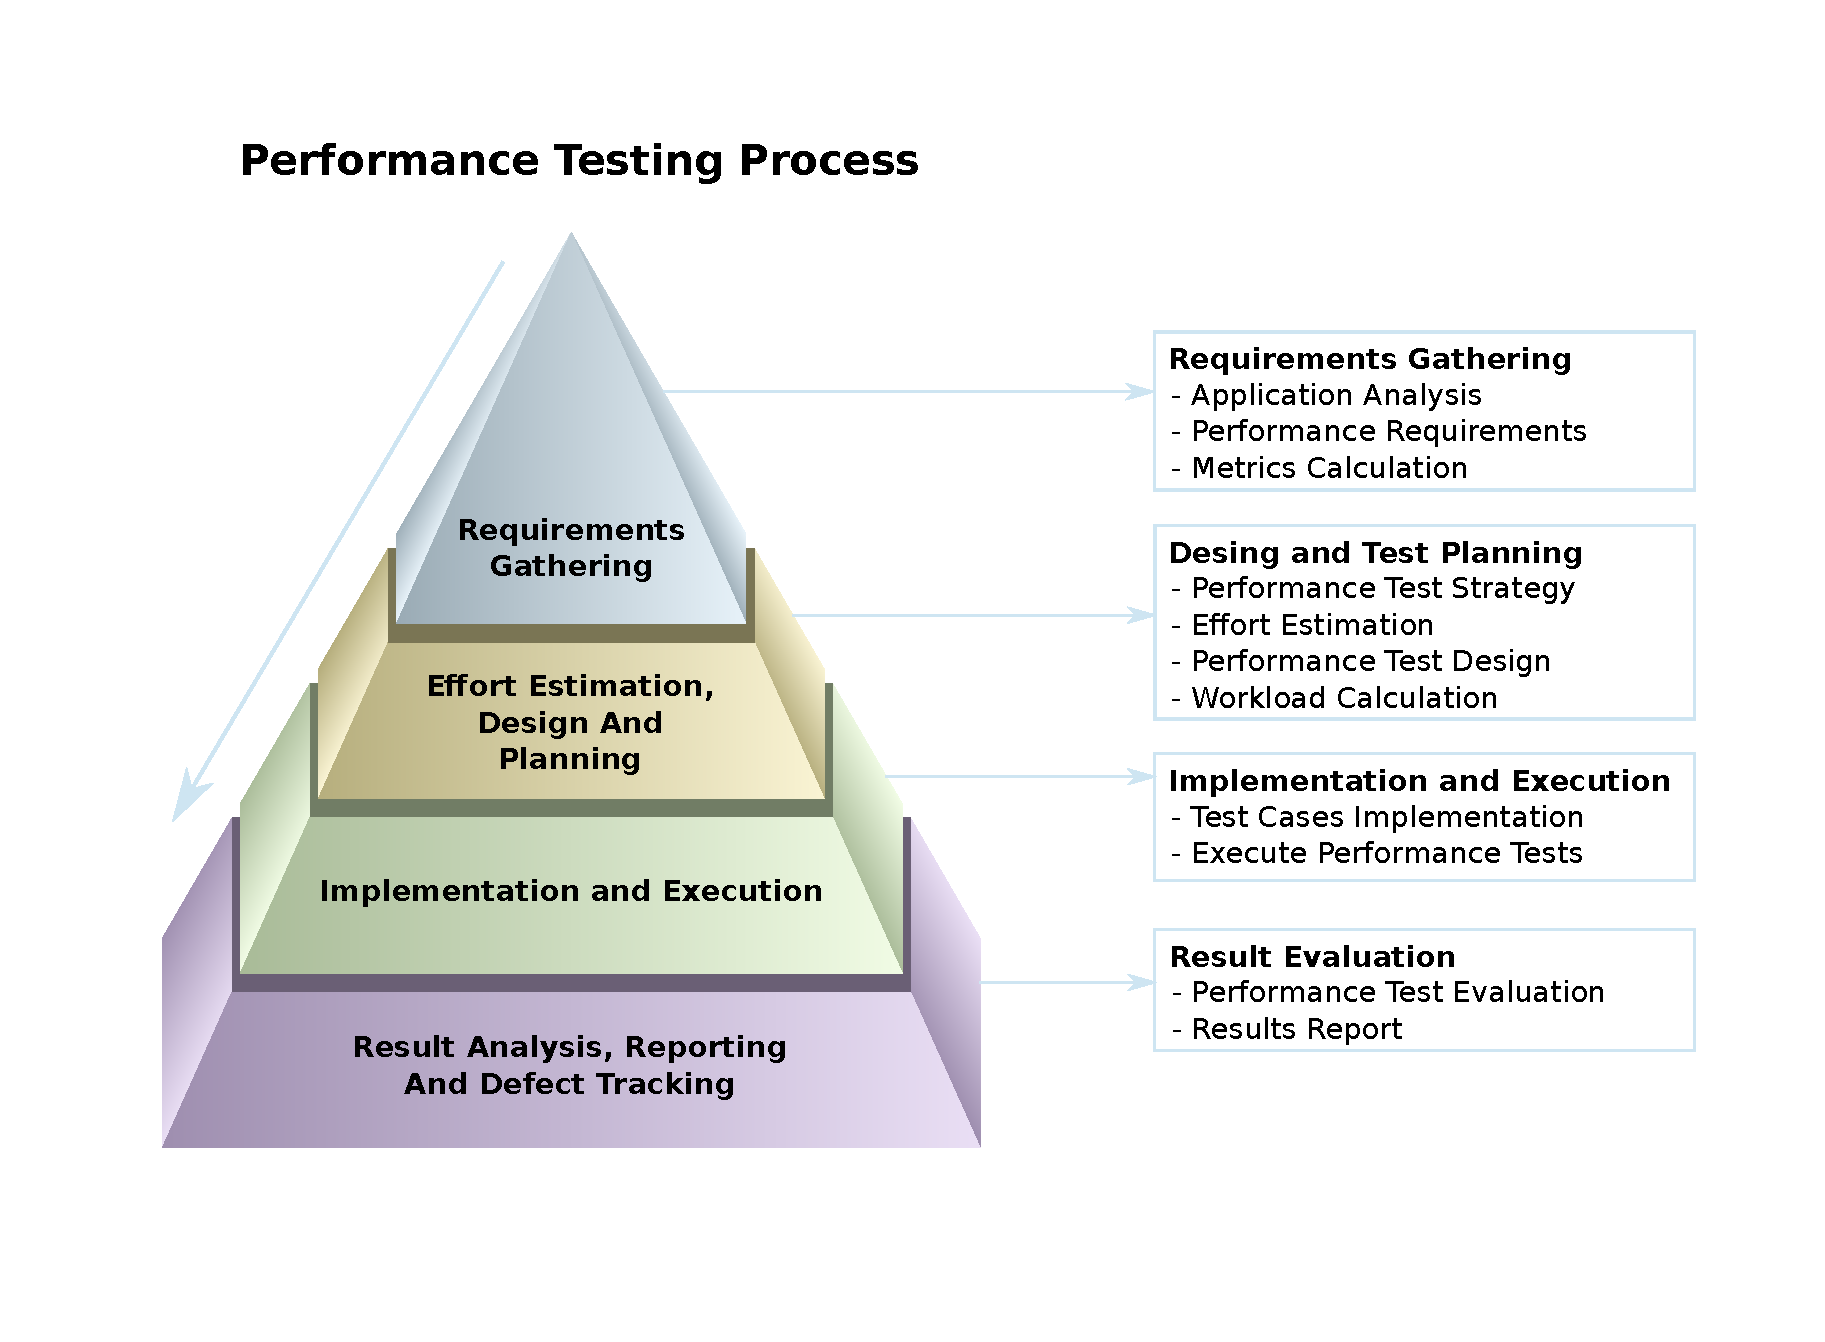
\includegraphics[width=16cm]{obrazky-figures/pyramid.pdf}
  \captionsetup{justification=centering}
  \caption{Performance Testing Process with the four most important parts and theirs individual steps based on \cite{Sharma:HP}.}
  \label{fig:performace_testing_process}
\end{figure}
In the Figure \ref{fig:performace_testing_process} you can see scheme of performance testing process where each level represent time for each step. Lower level refer to more time spend on that step.

The first step of performance testing process is the selection of \emph{performance requirements} for the application. In this step, testing engineer has to analyze \emph{software under test - SUT}, suitable performance metrics, that will model the application performance, and set performance requirements usually with customer and project manager. The result should include answers to questions such as:

\begin{itemize}
	\setlength\itemsep{0em}
	\item How many end users will the application need to handle at release, after 6~months or in 1 year ?
	\item Where will these users be physically located, and how will they connect to the application?
	\item How many end users will be concurrently connected in average at release, after 6~months and 1 year?
\end{itemize}

Based on answer to these studies, the engineer should be able to select important key performance indicators for performance test cases. Some of these indicators may be \emph{response time}, \emph{stability}, \emph{scalability}, or \emph{speed}. However, there is huge amount of possible indicators so it is necessary to properly analyze the whole application and also take into consideration another needs like an error rate, system resources, etc.  Result of this phase should be a~binding document with all performance requirements to be tested and, in case of detected performance degradation, such defect must be fixed with reference to this document.

The next step is to define the \emph{performance testing strategy}, corresponding to planning and design. It is extremely important to allocate enough time for SUT testing effectively, because, as it was mentioned in Chapter \ref{Introduction}, performance testing is not an easy task and detecting all of the possible issues of tested components is very time consuming process. Every plan should take into account the following considerations:

\begin{description}
	\setlength\itemsep{0em}
	\item \textbf{Prepare the test environment}\,---\,this step include choosing right hardware for testing, then installing the necessary software for running load injectors, tested components, etc., and other equipment depend on application purpose such as routers, switchers, mobile devices, etc.
	\item \textbf{Provide sufficient workload injectors}\,---\,preparing the workload injector may take few days; we usually requires a few workstations or servers to simulate real traffic.
	\item \textbf{Identify and implement use cases}\,---\,this include identification of important parts of the system which may have an impact on performance; time needed for each use case may be different because some use cases can be simple such as navigating to a web application home page, but some may be complex such as filtering specific communication.
	\item \textbf{Instrument the test environment}\,---\,install and configure the monitoring software on the test environment.
	\item \textbf{Deal with detected problems}\,---\,test can detect significant performance issues, but their investigation and fix may take a long time. After fix the retest of issue is needed.
\end{description}

While this process seems trivial, the opposite is true, in especially in case of network applications. Most of performance issues manifest at big workloads or high number of users, e.g. when million users are sending requests to the network device at the same time it could lead to an unacceptable device crash. Workload injectors are designated to simulate real user activity, and allows automatic analysis of performance behavior for tested application or device. Depending on the used technology, there can be a limit on the number of virtual users that can be generated by a single injector. These automated workload injectors are necessary for effective performance testing.

After describing the plan we implement and execute proposed test cases. Environment and workload injectors are ready for execution, so last step before the testing itself is the implementation of tests. Thanks to the careful planing, engineers should have enough time to implement test cases with reference to proposed design.

Final step of performance testing process is results evaluation. Output of this step is usually technical report with all selected performance key indicators, used workload and Collected Data Format for each test case. Then follows the data evaluation with thorough analysis of degradation localization. Additionally, the report usually contains syntactical graphs which display performance metrics along the duration of test execution.

\section{Performance Issues}
\label{Performance Issues}
\emph{Performance issue} is a common label for an unexpected application or device behavior which affects its performance. Usually, those issues are hard to detect because they manifest only under certain circumstances such as high load or long application run time. In the network applications there are several particular issues that are more frequently occurring  than others. In following, I~will describe selected issues in more detail.

\subsection*{Performance Degradation}
\label{Performance Degradation}
Unclean code usually leads to inefficient algorithms, application deadlocks, or memory leaks, which all can eventually cause the performance degradation. The problem is that these issues are usually detected only during the long run time of application or inability of an application to handle high load. For this kind of issues there is a performance testing method called \emph{soak testing} \cite{BUCH:4TYPES, Manzor:APTB} which is described in Section \ref{Endurance Testing}. Soak test is intended to identify problems that may appear only after long period of application run-time\footnotemark{}, hence its necessary to run this type of tests during application development. The network applications are usually need to be available for 24 hours per day. The duration of a soak test should have some correlation to the operational mode of the system under test. Following scenarios may represent performance issues detectable by soak tests:

\begin{itemize}
	\setlength\itemsep{0em}
	\item a constant degradation in response time, when the system is run over the time,
	\item any degradation in system resources that are not apparent during short runs but will surface during long run time such as free disk space, or memory consumption
	\item a periodical process that may affect the performance of the system, but can be detected only during long run time as backup process, exporting of data to a 3rd party system, etc.,
	\item development of new features for already exists components.
\end{itemize}

\footnotetext{Soak Test - refer to HW testing method during which engineers soak device into water and check for bubble leaks.}

\subsection*{Response Time}
\label{Response Time 1}
Response time is how long it takes system to accept, evaluate, and respond to the user for his request e.g. HTTP request for particular website. Different actions and requests can have significantly different response time and with that provide different load on the system. For example retrieving document from web-server by its ID is considerably faster than searching for the same document by keywords. Response time is mostly measured during the \emph{load test} \cite{Manzor:APTB} of the application. Well designed test should consider different types of load on the system, various kind of requests, and different number of connected end-users at the same time. For user based systems we usually consider 3 threshold for the response time values:

\begin{description}
	\setlength\itemsep{0em}
	\item \textbf{0.1 second}\,---\,this represent an ideal response time for the application, because user feels that system is reacting instantly and does not notice any interruptions.
	\item \textbf{1 second}\,---\,this is the highest acceptable response time when user still does not feel any interruptions, but can feel a little delay; this still represent no bad impact on the user experience.
	\item \textbf{10 second}\,---\,this is the limit after which response time become unacceptable and user will probably stop using your application.
\end{description}

However response time limits for non-human interactive system are more strict. They could acquire values in milliseconds or less.

\todo{Prvni iterace}

\subsection*{Traffic Spikes}
As \emph{traffic spike} \cite{Kurkova:Thesis:2017, AMC:SPIKES} we can understand the sudden surge in demand from users. Typically doubling or multiplying of traffic level in short period of time. In real network, spikes are result of high workload, e.g. caused by higher amount of users trying to concurrently use the service over the network. For example we can experience sudden traffic spike in response time after publishing new popular viral context on video servers, start of sales events, reservation of limited amount of tickets or subject registration at university. Scheduled automatic backup or system upgrade for whole company during early morning hours can cause traffic spikes.

Traffic spikes can lead to inappropriate system behavior such as \emph{long response time}, \emph{bad throughput}, and \emph{limited concurrency}. To prevent the impact of traffic spikes on system performance, it is  necessary to do sophisticated infrastructure monitoring and network load analysis, in order to distinguish between normal traffic and attack on the system. Suitable methods for testing of spikes is one of variant of \emph{stress testing} \cite{Manzor:APTB} and it is described in Section \ref{Types of Performance Testing} in more details. Network system should offer load balancing, thus it should be able to redirect traffic to another node with same service in case of high load which can cause performance issues due inappropriate resource usage.

\begin{figure}[H]
  \centering
  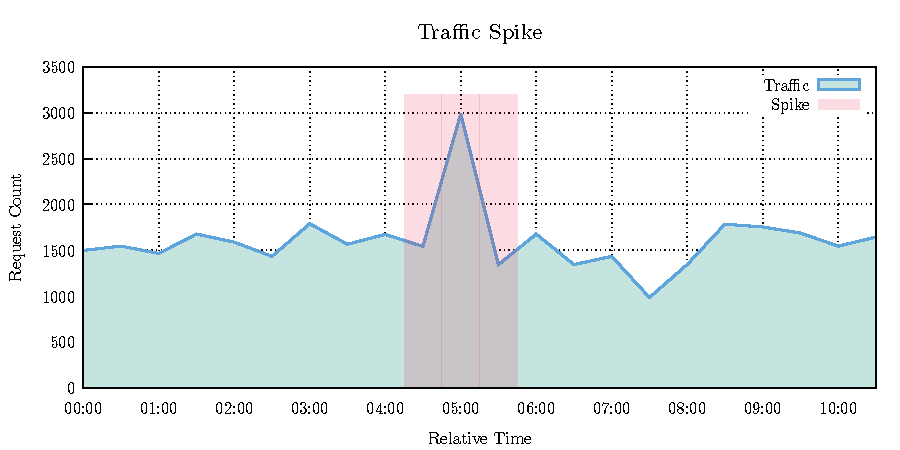
\includegraphics[width=14cm]{obrazky-figures/traffic_spike.pdf}
  \caption{The graph shows amount of concurrent sessions depending on time. During to network traffic monitoring the traffic spike occurring after 5 hours from test start.}
  \label{fig:spikes}
\end{figure}

\section{Types of Performance Testing}
\label{Types of Performance Testing}
% % http://www.wmrichards.com/high_performance_messaging.pdf 2017/10/18

For performance testing there are many types of suitable test methods. Which test you should use is determined by the nature of the system, testing requirements or how much time we have left for the performance testing. The following terms are generally well known and used in practice and each of them characterizes category or suite of the tests:
\begin{itemize}
	\item \textbf{Testing methods}\,---\,load testing, stress testing, endurance testing, \todo{scalability, volume, recovery}
	\item \textbf{Testing approaches}\,---\,smoke testing, regression testing, benchmark testing
\end{itemize}

Their description is based on knowledge available in \cite{TuPo:TESTS, BUCH:4TYPES, Molyneaux:TAoAPT, ISTQB}.

\subsection*{Load Testing}
Finding maximal load is a testing method which studies how the system behaves during different types of workload within acceptable time range. Basically it simulates the real-world load. During the load test we mainly focus on metric response time of the system for requests. Requests are generated by users or another systems communicating with the SUT. Main goal is to determine if the system can handle required workload according to performance requirements. Load test is designed to measure the response time of system transactions under normal or peak workload. When the response time of the system dramatically increases or becomes unstable, we conclude that system reached its maximum operating capacity. After successful testing, we should mark the workload requirements as fulfilling or analyze Collected Data Format and report issues to the developers. In the Figure \ref{fig:load_test} you can see the graph of load test showing workload of raising requests to the web server at the same time where the system response time does not exceed 3.5 seconds.

\begin{figure}[H]
  \centering
  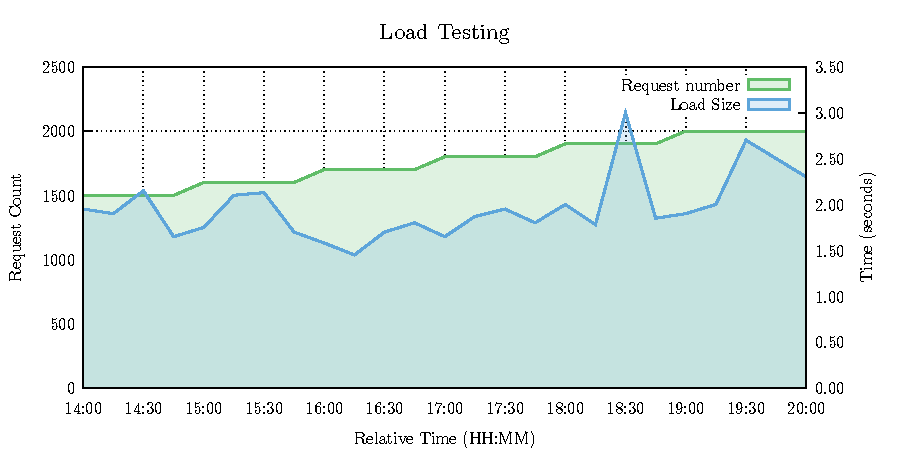
\includegraphics[width=15cm]{obrazky-figures/load_testing.pdf}
  \caption{Response time of the system during the load testing depended on load size.}
  \label{fig:load_test}
\end{figure}

The following lists show common scenarios for load testing:
\begin{itemize}
	\setlength\itemsep{0em}
	\item The system interact with multiple users at same time.
	\item The system tracking communication and analyze it.
	\item Web services and information systems.
\end{itemize}
Typical system issues covered by load testing:
\begin{itemize}
	\setlength\itemsep{0em}
	\item Concurrent users connections can eventually result into slow response time or system crash.
	\item Network systems without redundancy connections can shutdown whole network under normal defined workload.
	\item Data availability during multiple session to data server.
	\item Connection rejection (timeout).
\end{itemize}

\subsection*{Stress Testing}
\label{Stress Testing}
Stress testing is the specific type of load testing, where we do not measure normal workload, but focus on unexpected workloads or traffic spikes. The main purpose is to study how the system behaves in extreme conditions such as enormous number of concurrent requests, using a server with much less memory or a weaker CPU, and analyze the system performance threshold. Its very useful to know performance threshold in order to know the difference between performance under normal workload and performance threshold. The following enumeration lists common stress test scenarios:
\begin{itemize}
	\setlength\itemsep{0em}
	\item Monitor the system behavior with over maximum of users logged in at the same time.
	\item All user performing critical operations at the same time.
	\item All users accessing the same file at the same time.
	\item Hardware issues such as server in cluster down.
\end{itemize}
Typical issues, which are covered by stress testing:
\begin{itemize}
	\setlength\itemsep{0em}
	\item Sudden performance degradation.
	\item System will recover after stress test (system is operational after test).
	\item System does not crash during stress test.
	\item All subsystems such as database, load balancer, etc. remains operational.
\end{itemize}

When engineers finish stress testing and found the limits of the system, they also can test the system recovery after crash during finding of the system limits.

In the Figure \ref{fig:stress_test} is recorded stress testing with raising load and response time. Everything is fine until the amount of requests exceed 3000 requests per second. With higher load there comes performance issues which leads to unexpected rise of the response time.

\begin{figure}[H]
  \centering
  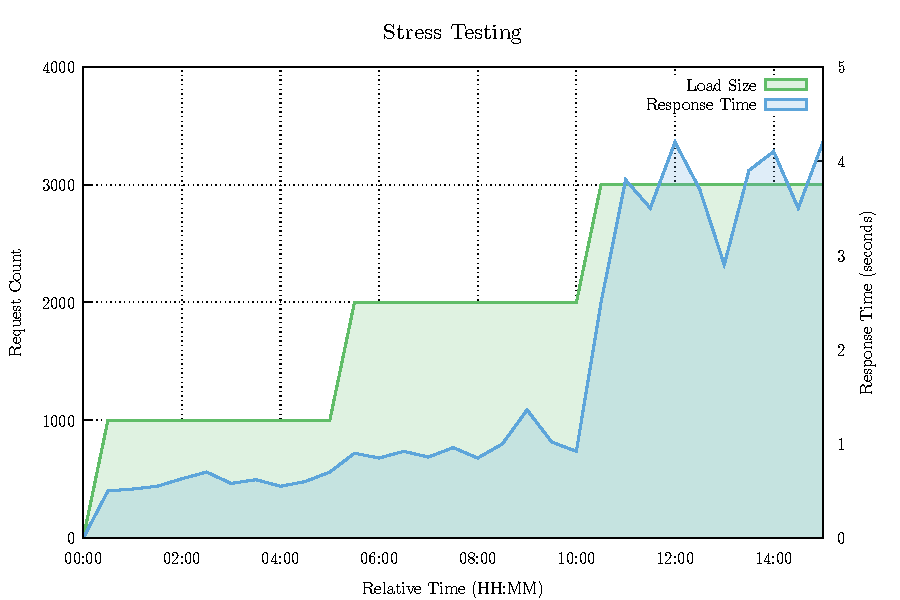
\includegraphics[width=15cm]{obrazky-figures/stress_testing.pdf}
  \caption{Stress testing diagram capturing dependency of response time on amount of requests.}
  \label{fig:stress_test}
\end{figure}

\subsection*{Endurance Testing}
\label{Endurance Testing}
Endurance, or stability/soak testing refer to the method, that tries to identify problems, that may appear only after the extended period of time e.g. The system could seems stable for one week, but after some longer period, problems such as memory leaks or not enough disk space can appear. Soak tests mainly focuses on measuring of memory as performance metric. The following are common issues found by soak test:
\begin{itemize}
	\setlength\itemsep{0em}
	\item Serious memory leaks that can eventually result into the system crash.
	\item Improperly closed database connections that could starve the system.
	\item Improperly closed connections between system layers that could stall any of the system modules.
	\item Step-wise degradation that could lead to high response time and the system becomes inefficient.
\end{itemize}
Typical scenarios for use soak testing:
\begin{itemize}
	\setlength\itemsep{0em}
	\item Developed system uses multiple database connections.
	\item There is a chance for inappropriately allocated memory, and memory free.
	\item Disk space limitation for store logs or other data.
\end{itemize}


This sort of test needs to use appropriate monitoring system to achieve high efficiency. Problems detected by soak tests are typically manifested by gradual system slowdown in response time or as a sudden lost of system availability.

\begin{figure}[H]
  \centering
  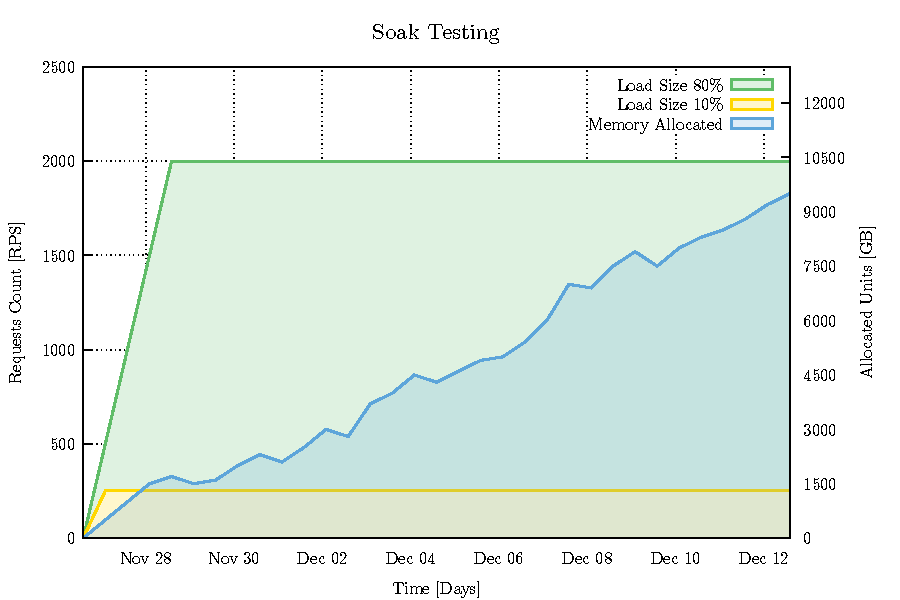
\includegraphics[width=15cm]{obrazky-figures/soak_testing.pdf}
  \caption{Soak testing with memory usage dependent on time.}
  \label{fig:soak_test}
\end{figure}

In the Figure \ref{fig:soak_test} you can see raising memory usage after period of time. The SUT can handle requests but as time goes by memory usage is too high that the SUT will crash. This may be caused by memory leak or an inappropriate algorithm use.

\subsection*{Smoke Testing}
Smoke testing approach is inspired by similar hardware technique, when engineers checks for presource of the smoke from the device after turning the power on. Basically, its similar for software, since main goal of smoke test is to test basic functionality of the system and guarantee that the system is ready for build. However, smoke tests are testing the functionality on a surface level, so it may not be enough for deep testing of basic system functions. When smoke tests fail, the system is tagged as unstable, because it cannot ensure its basic functionality and it is not tested anymore until the smoke test pass. Smoke test are designed to uncover obvious errors which saves time, money and effort of the engineers. These tests should be used with every new build, since new features could harm previous system functionality.
The following lists show common scenarios for smoke testing:
\begin{itemize}
	\setlength\itemsep{0em}
	\item New system's build or version is ready for further testing or productilization.
\end{itemize}
Typical system issues covered by smoke testing testing:
\begin{itemize}
	\setlength\itemsep{0em}
	\item System without main functionality is useless, because test coverage of functionality is low.
	\item Main functionality can result into system crash.
\end{itemize}

Smoke testing is not typical performance testing approach, but it can be used for initial load test for check if system can be started.

%\footnotetext[\label{note1}]{Approach for test suits, where are used other methods like Load testing, Stress testing, etc.}

\subsection*{Regression Testing}
Whenever engineers develop new feature and want to update the previous build it has to pass the \emph{regression tests}\footnote{Approach for test suits, where are used other methods like Load testing, Stress testing, etc.}\addtocounter{footnote}{-1}\addtocounter{Hfootnote}{-1} \cite{STF:REGRESSION}. Regression tests are designed to test functionality of the latest build updated with new feature. The main objective is to determine, if new feature affects already functional parts of the system. This type of tests is very important, because engineers do not always realize, which parts of the system will be indirectly affected. During regression testing, new test cases are not created, but previous test cases are automatic re-executed and analyzed.
Typical scenarios for regression testing:
\begin{itemize}
	\setlength\itemsep{0em}
	\item New feature of system is ready for use.
\end{itemize}
Common issues covered by regression testing:
\begin{itemize}
	\setlength\itemsep{0em}
	\item New feature could adversely affect already working components of the system.
\end{itemize}

%\footnotetext{Approach for test suits, where are used other methods like Load testing, Stress testing, etc.}

\subsection*{Benchmark Testing}
\emph{Benchmark testing}\footnotemark{} is approach, which collects performance data during the system run on different hardware machines \cite{Aho:Benchmarking}. Collected Data Format have significant value when we want smooth run of the system on an older hardware, hence we can discover performance issues under normal load. However, the system does not run smoothly on prepared hardware, only options is to run benchmark tests on different machines with different hardware and under different load.

\begin{itemize}
	\item Can identify minimal requirements for HW, metrics, etc.
	\item Can validate supported HW configuration.
\end{itemize}



\section{Performance Metrics}
\label{Performance Metrics}
% https://loadstorm.com/load-testing-metrics/ 2017/10/18

During the performance testing we can monitor a lot of metrics, which can have different importance based on the system's purpose. The following lists the most common metrics that are monitored during the performance testing of all applications, no matter of developing language.

In the testing systems, performance metrics are collected during long process of collecting, analyzing and reporting information regarding performance of whole system or individual component. This process can be different for each metric, since each metric needs different type of the system analysis.

\subsection*{How to Measure}
Performance measurement process can be divided into several steps. Metrics are usually measured after a warm-up period of time after the commencement of traffic, because it takes a while for workload to stabilize. Stabilized workload is necessary for measurements because unstable workload can negatively affect the measurement results. In the Figure \ref{fig:measurements} you can see workload phases with marked part for the performance testing.

\begin{figure}[H]
  \centering
  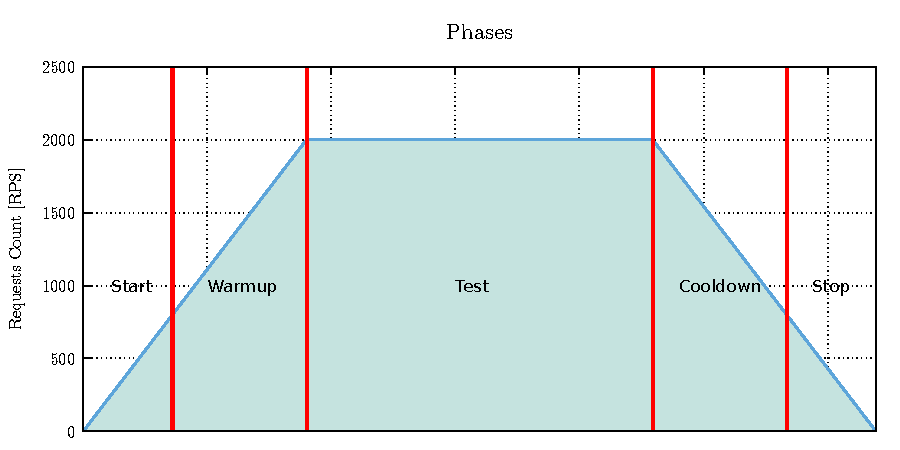
\includegraphics[width=15cm]{obrazky-figures/measure_demo.pdf}
  \caption{Load phases of performance measurement process.}
  \label{fig:measurements}
\end{figure}

Workload during testing does not have to be on the same value during whole testing. In particular, load testing finds the highest load during which the system can work properly. This limit is find by raising the load and monitor the system as it is shown in the Figure \ref{fig:load_test}.

\subsection{Throughput}
Throughput is a metric, which refers to the number of requests per second that the system can handle. \emph{Network throughput} is the rate of successful message deliveries over a communication channel. Throughput is measured by load testing; suitable strategy for measuring throughput is to continuously raise the load until response takes longer that acceptable threshold. \todo{neco dopsat}

\subsection{Response Time and Latency}
Response time as issue was already mentioned in Subsection \ref{Response Time 1}; response time as metric is consists of two parts which are \emph{latency} and \emph{service time}.

\subsubsection*{Service Time}
Service time is the time it takes system to evaluate and send response to user request. In particular, when user sends request for a web page to a server, it takes the server time to evaluate the request and send proper response back to the user, this is the service time. Measurement can be performed easily using stopwatch which starts at receive of request and stops after the response is send. Service time can be affected by any item which leads to a performance degradation as described in Subsection \ref{Performance Degradation}.

\subsubsection*{Latency}
The second part of the response time is latency \cite{Broadwell:RPT, BHATT:PERF}, which represent a delay between sending the request on the client side and receiving it for evaluation on the server side. Hence latency is the common problem in the network systems such as data center, web server, etc., because request/response needs to travel over the physical medium between the client and the server. Client and server could be located on different continents, thus the message have to travel long distance and latency is increasing.

\subsubsection{Round Trip Time}
Round-trip time (RTT) is time that it takes for a signal to be sent with time it takes for an acknowledgement of that signal to be received. In network, the RTT is one of the several factors that affects the signal latency. Basically, RTT is depends on the distance between sender and receiver, because that distance the signals must be travel by.


\begin{figure}[H]
  \centering
  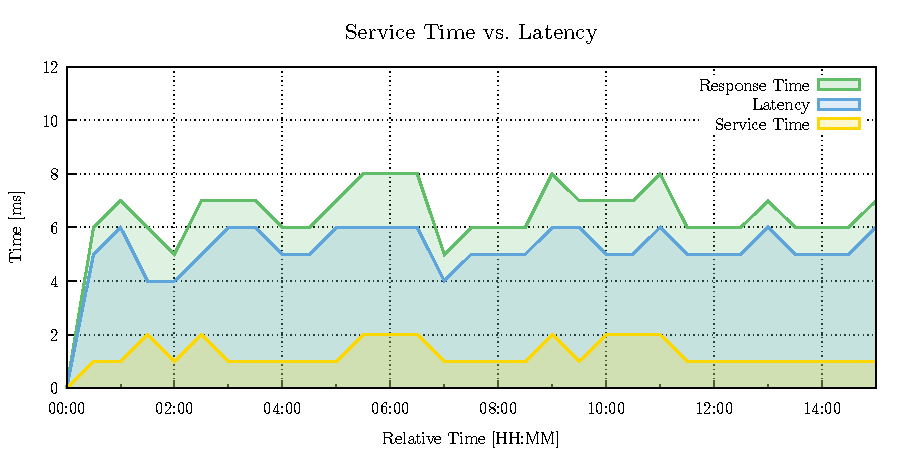
\includegraphics[width=15cm]{obrazky-figures/latency.pdf}
  \caption{Diagram capturing diference between latency and response time.}
  \label{fig:latency_vs_service_time}
\end{figure}

In the Figure \ref{fig:latency_vs_service_time} you can see response time and both it parts: latency and service time. Service time is usually smaller than latency since latency depends on distance. When you add service time value and latency value you will get response time at certain time.

\subsubsection*{Average and Percentile Response Time}
There are two common ways of measuring the response time \cite{Kopp:RPT}: Average (mean) response time is calculated as the sum of all measured times divided by the count of users requests. While this seems trivial, in many times, the average response time does not actually reflect the real response time of the system. How is that possible? In reality, most application have few heavy outliers such as very slow transactions. In the Figure \ref{fig:average_percentil_1} you can see few slow transactions which drag the average of the response time to the right. This naturally leads to an inaccurate specification of response time.


\begin{figure}[H]
  \centering
  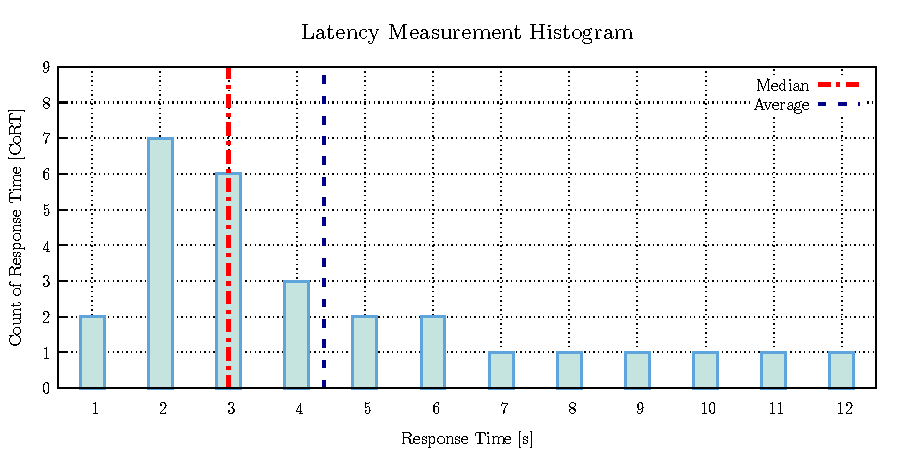
\includegraphics[width=15cm]{obrazky-figures/average_median_1.pdf}
  \caption{Transactions response time with calculated average and median of response time.}
  \label{fig:average_percentil_1}
\end{figure}
In the Figure \ref{fig:average_percentil_1} the average represent inaccurate response time, which is higher than real one.

The better solution how to determine the actual response time is Percentile. The percentile is statistic method, which cut measured ordered values into hundredths and then characterize the value below which a given percentage of measurements in a group of particular measurements falls. In the Figure \ref{fig:average_percentil_1} you can see the \emph{median} value, which reflects more realistic value of the system response time. Median value is same such as the 50th percentile. In this case, there is no problem, because user will expect slower response time than it has.

\begin{figure}[H]
  \centering
  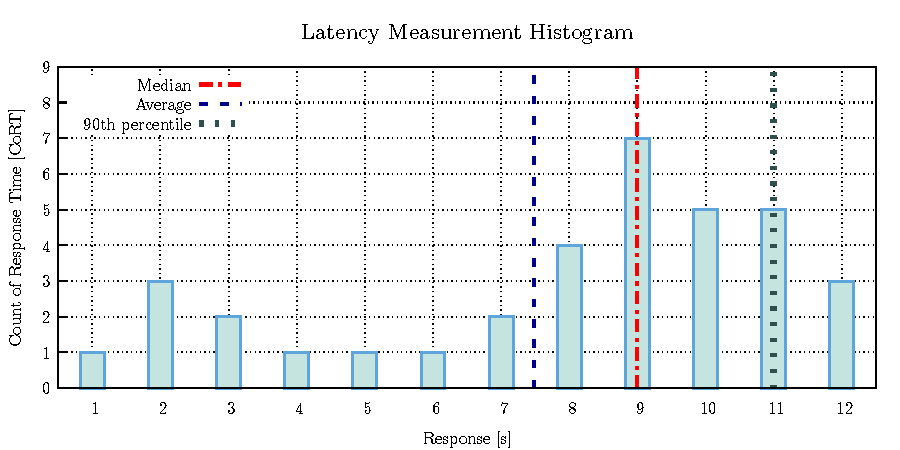
\includegraphics[width=15cm]{obrazky-figures/average_median_2.pdf}
  \caption{Transactions response time with calculated average and median of response time.}
  \label{fig:average_percentil_2}
\end{figure}

The Figure \ref{fig:average_percentil_2} shows different situation. Average represent inaccurate response time, which says, that STU is faster than is in reality. Average response time seems better than median, which reflects the expectation of faster system response time than it has. In real systems, we usually use values of the 90th percentile and the 99th percentile. 90th percentile mean, that there is only 10 \% transactions slower then marked response time. In the Figure \ref{fig:average_percentil_2}, a considerable percentage of transactions are very fast (first 50 percent), while the bulk of transactions are several times slower. Thus, calculated percentile gets more realistic values than average response time.

\subsection{Resource Usage}
Applications running at servers with long run-time competes over a limited amount of resource available for use. Thus makes resource usage another important metric, which needs to be monitored since not enough resources could shut down the whole system. Main resources for monitoring and utilization are:

\begin{description}
	\setlength\itemsep{0em}
	\item \textbf{CPU usage}\,---\,inappropriate usage of CPU could lead to performance degradation, because low priority processes may occupy CPU ahead of the higher priority processes. CPU usage is structuring into system usage and user usage. High system usage can cause problems or bottlenecks.
	\item \textbf{Memory usage}\,---\,full consumption of memory could cause performance degradation.
	\item \textbf{Disk space}\,---\,for example when using storage disk as a database, there should be preventive measures to backup the data and free up disk space.
	\item \textbf{Operating System limits}\,---\,system's memory, and CPU capabilities.
\end{description}


\subsection{Error Rate}
Error Rate is a~metric, which commonly occurs in the network systems, especially under high load. During the communication between client and server there could be error caused by another network device (router, switch, etc.) or signal disruption of the data during the transfer. The Error Rate is the mathematical calculation that produces a percentage of problem requests compared to all requests. In the ideal system, there should be zero network error present, however, in reality is in-feasible. This usually leads to a performance degradation and low throughput, because damaged data need to be resent.
Error rate is a~significant metric because it tells engineers how many requests failed at a particular point in time of performance testing. This metric is more evident when you can see the percentage of problem strongly increasing, hence you can detect problem easily.


\todo{Druha iterace}

  % (c) Jakub Stejskal
% Master Thesis
% Performance Testing and Analysis of Qpid-Dispatch Router
% Chapter 3

\chapter{Messaging Performance Tool}
\label{Messaging Performance Tool}
% https://github.com/orpiske/msg-perf-tool
The performance of \emph{Message-Oriented Middleware} (MOM) \cite{CURRY:MOM} is one of the most critical elements of quality assurance for enterprise integration systems. There are multiple messaging components developed in the Red~Hat~Inc. company such as messaging clients, message broker, message router (Qpid-Dispatch service) or stream-like message distributions tools---Kafka. All of these software needs performance testing to ensure quality standards of MOM. Note that we will shorten the term the messaging client to just client in this thesis.

The~message broker is an example of MOM. Its main purpose is to receive, store and distribute messages, which are sent and received by clients. Users choose MOM for message distribution to reduce the development time and cost of their own solution. Another benefit of using specialized MOM is robustness and guaranteed performance. The performance capabilities of a MOM are critical attributes to its users, because being able to handle a large amount of transactions in a timely manner is a key characteristic of MOM. Good example are automated systems, where components communicates with each other by command exchange. The amount of exchanged commands is heavily dependent on the system size and since we want to get the results as soon as possible we need to ensure smooth and quick message exchange.

\emph{Maestro} (or Messaging Performance Tool) \cite{ORPISKE:MSGPT} is a testing system designed for testing the performance of MOM. The Maestro is deployed as a cluster system on several machines. A~typical deployment consist of one node for Maestro Broker, one or more for Maestro Senders, and one or more for Maestro Receivers and the SUT. The architecture of Maestro system, depicted in the Figure \ref{fig:msg_perf_tool}, consists of the following components:

\begin{description}
	\setlength\itemsep{0em}
	\item \textbf{Maestro Broker}\,---\,can be any \emph{Message Queuing Telemetry Transport\footnote{MQTT\,---\,\url{http://mqtt.org/}} (MQTT)} capable broker with several topics. The topic is a queue with a name where other messaging services can listen on the traffic. This component takes care of distribution of control messages between other cluster components such as Maestro Clients and MPT Backend.
	\item \textbf{Meastro Clients}\,---\,this component contains the client API as well as the test scripts for each test case. Moreover it contains a~sub-component called Reporter which interprets the test data to user in form of web data visualizations.
	\item \textbf{MPT Back-end}\,---\,consists of sender, receiver and inspector parts. Sender and receiver handle message sending to the SUT and receiving from SUT. Inspector monitors workload over the SUT and reports collected performance metrics to the data server. Maestro currently has two backends:
	\begin{itemize}
		\item \textbf{Java}\,---\,used for JMS-based\footnote{JMS\,---\,Java Message Service} testing, including \emph{Advanced Message Queuing Protocol (AMQP)} \cite{OASIS:AMQP}, OpenWire and Core protocols.
		\item \textbf{C}\,---\,used for AMQP and \emph{Streaming Text Oriented Messaging Protocol\footnote{STOMP\,---\,\url{https://stomp.github.io/}} (STOMP)} protocol testing.
	\end{itemize}
\end{description}

\begin{figure}[H]
  \centering
  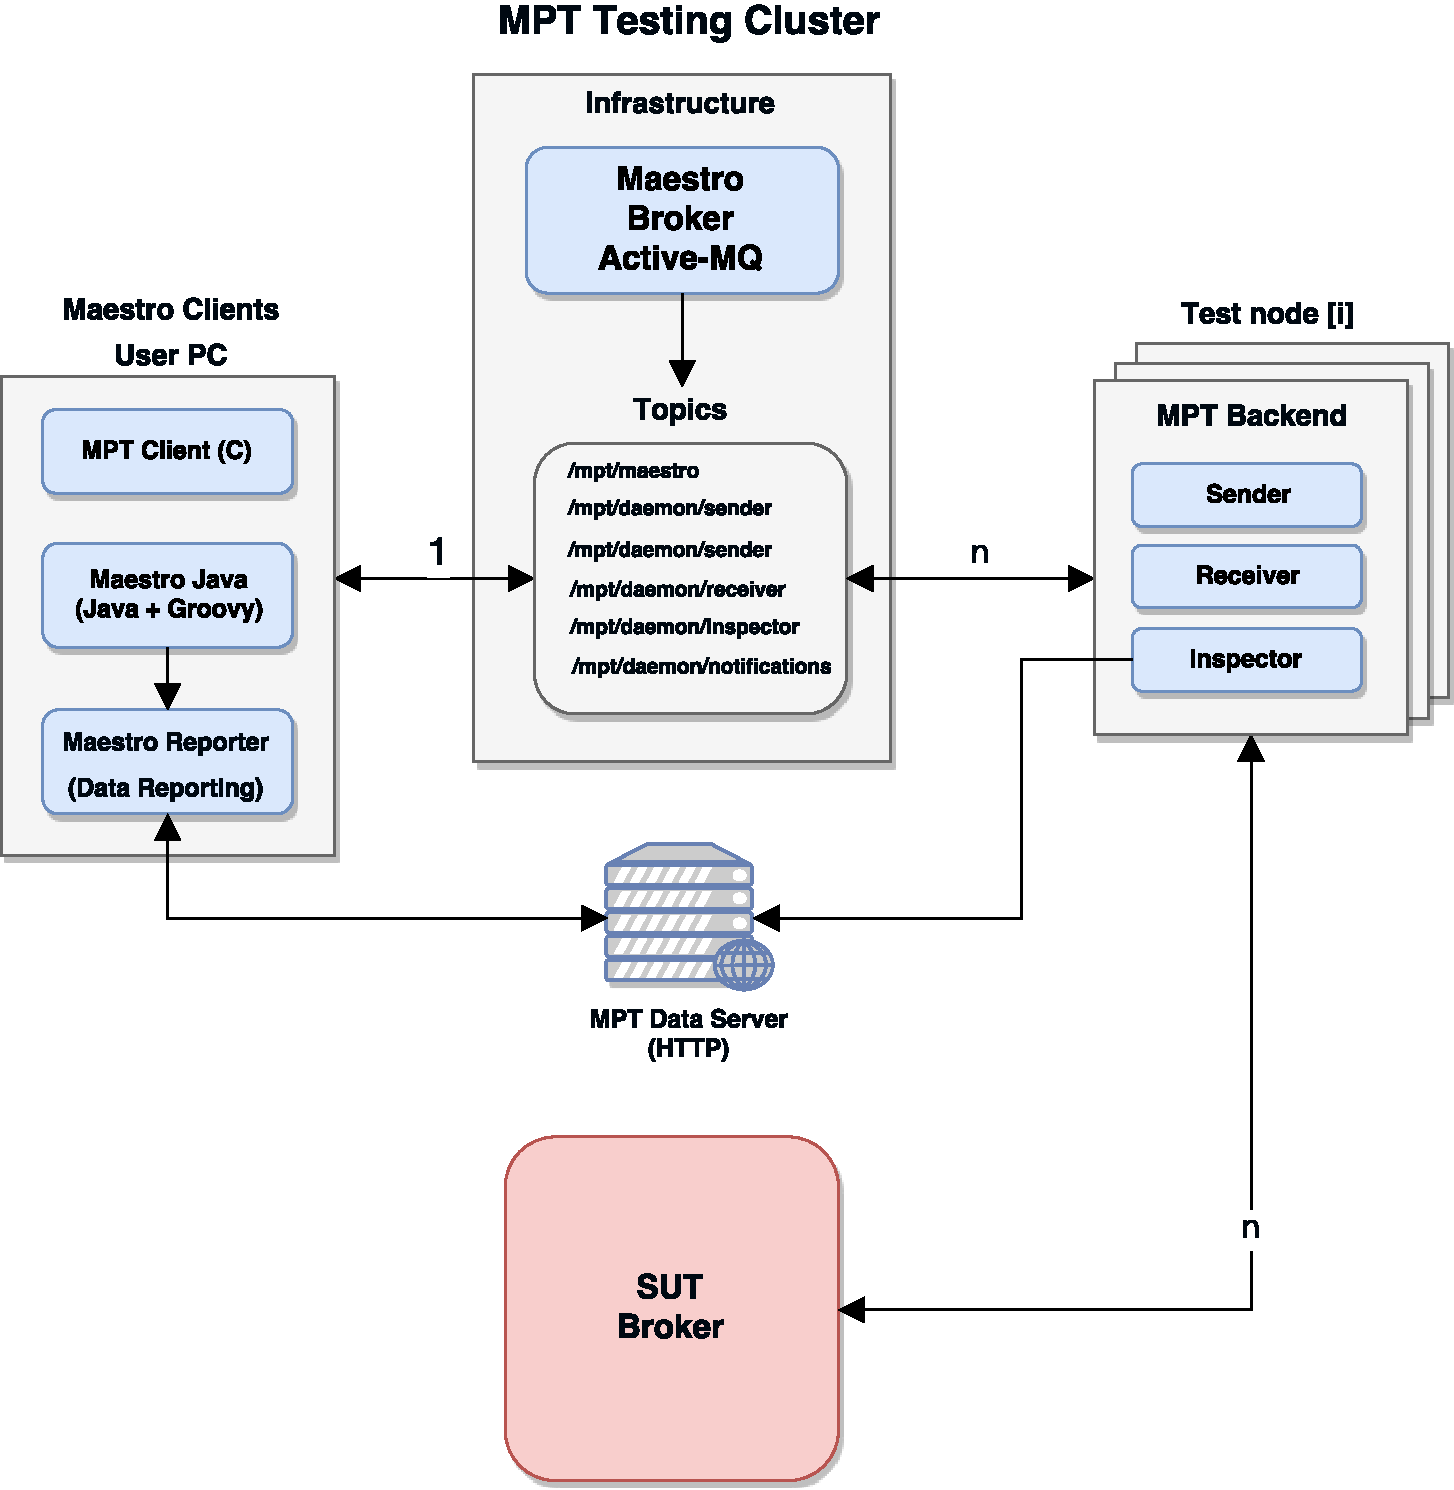
\includegraphics[width=15cm]{obrazky-figures/msg_perf_tool.pdf}
  \caption{The architecture of the Maestro. The Maestro contains Maestro Clients as a front-end; Maestro Broker as a message distributor; and sender, receiver and inspectors as a backend. The arrows represent communications between the Maestro components and with the SUT. The line value represents the number of connections where default is 1.}
  \label{fig:msg_perf_tool}
\end{figure}

\newpage

\section{Test Case Scenario}
The test is basically a generation of huge amount of messages followed by sending them to SUT and then receiving them. The configuration of each test case is specified by several options defined in the Groovy\footnote{Groovy\,---\,object-oriented programming language for Java platform \url{http://groovy-lang.org/}} script which influences the test behavior with the following elements:

\begin{itemize}
	\setlength\itemsep{0em}
	\item \textbf{message size}\,---\,size of the generated test message in bytes,
	\item \textbf{number of connected clients}\,---\,the count of senders and receivers connected to the SUT,
	\item \textbf{test duration (time or load)}\,---\,the end condition of each test; can be specified by time, limit or message count,
	\item \textbf{message rate}\,---\,the desired rate that the system should try to maintain through the test (0 for unbounded rate).
\end{itemize}

The test script is also responsible for starting and stopping the test. Moreover the test case can be extended by the so called test profile. The script will then also be responsible for increasing or decreasing the workload on the SUT during the test scenario. This load can be modified by increasing either the target rate or the number of parallel connections. With multiple combinations of these options we can create a lot of test cases with different loads for the SUT and thus achieve a broad coverage of testing. Every test produces its own logs which are processed by the reporting sub-component on the client side and used for monitoring the metrics. Maestro Reporter produces data visualizations, such as the test overview and charts (rate based on time and latency over the test) from these logs.

\section{Communication Between Components}
\label{Communication Between Components}
The actual communication between components during the test cases is realized using the Maestro Protocol\,---\,a binary protocol implemented on top of the MessagePack\footnotemark{}. For the message exchange between nodes it currently uses MQTT protocol (version 3.1.1) and for sending the testing data to the data server it uses HTTP protocol (version 1.1). The messages exchanged between the peers of testing cluster are called notes.

\footnotetext{Messagepack\,---\,\url{https://msgpack.org/}}

Each note has a specific format consisting of three parts. First is the \emph{Type} which is short integer that identifies the purpose of the note, and is one of the following values:

\begin{itemize}
	\setlength\itemsep{0em}
	\item \textbf{Request (0)}\,---\,a note sent by a controller node to the test peers,
	\item \textbf{Response (1)}\,---\,a note sent by a testing peer as a response for a request,
	\item \textbf{Notification (2)}\,---\,a note sent by a testing peer as a reaction to an event.
\end{itemize}
The second part is the \emph{Command} which identifies the action to be executed or, in some cases, that was executed. Currently, there are 18 commands represented by a long integer. And the last part is the \emph{Payload} which refers to the data carried by the note as part of its command. Detailed description of commands and its payload is available in Appendix \ref{AP:commands}.


\section{Measuring Process}
\label{Measuring Process}
After the dynamic test generation, with options from the test file, the measuring process starts. Senders will start sending messages to the SUT, while Inspector starts monitoring the behavior of the SUT and sends measured data to the data server. For monitoring purpose, Inspector uses the Broker management interface\,---\,a REST interface that exposes (via HTTP protocol) an internal JVM\footnote{JVM\,---\,Java Virtual Machine} and Broker detailed information. The actual data collection by Inspector is straightforward:

\begin{enumerate}
	\setlength\itemsep{0em}
	\item Inspector sends a HTTP request with the \emph{JavaScript Object Notation\footnotemark{} (JSON)} content to the Broker REST interface.
	\item Broker evaluates the request and sends response to the Inspector.
	\item Inspector collects the response.
\end{enumerate}
Note that errors occurred during the collection may cause the test case to fail.

\footnotetext{JSON\,---\,\url{https://www.json.org/}}

However, there are two problem factors; the first is that the Inspector should not influence the performance of the SUT. Current solution for the information collection works like the management interface method call with request for information and response retrieval. During this call, the method usually involves locks to guarantee the thread safety and exclusive access. However, calling this method too often can cause a significant Broker performance degradation. In order to reduce this risk, the inspector enforces a collection interval of 10 seconds and restricts usage only to selected operations. This strategy reduces the hits on management interface to 2 or 3 hits every 10 seconds and presents a suitable performance.

The other problem factor is the large size of the stored logs. This is mitigated by the usage of the compression methods. However, compressed logs can still fill the whole hard drive during the long test-run and so old logs has to be erased at some point of time. Collected logs can be safely erased when the test is completed. Currently the Maestro generates about 1\,Gb of uncompressed data per hour of testing.

%Inspector also monitor node with broker (CPU, memory size)?

%No. There's a new module being developed for that, which runs on top of Prometheus and monitors both the system and the test cluster: http://msg-qe-dev-01.tpb.lab.eng.brq.redhat.com:3000


\subsection{Testing Metrics}
\label{Testing Metrics}
The type of metrics collected during tests depends on the cluster component. In the Table \ref{tab:maestro_metrics} we can see the summary of the metrics, which are collected for each component.

\begingroup
\setlength{\tabcolsep}{10pt} % Default value: 6pt
\renewcommand{\arraystretch}{1.35} % Default value: 1
	\begin{table}[H]
	\centering
	\begin{tabular}{|p{2.5cm}|p{3.5cm}|p{7cm}|}
	\hline
	\rowcolor[HTML]{C5E3DF}
	\multicolumn{1}{|c|}{\textbf{Component}} & \multicolumn{1}{c|}{\textbf{Metrics}} & \multicolumn{1}{c|}{\textbf{Description}}                       \\ \hline
	\textbf{Sender}                          & Throughput                            & Throughput of the sender                                        \\ \hline
	\textbf{Receiver}                        & Throughput                            & Throughput of the receiver                                      \\ \hline
	\textbf{}                                & Latency                               & Time between send and receive messages                           \\ \hline
	\textbf{Broker}			                & JVM heap memory                       & Maximum, minimum, and current Eden, Survivor, and Tenured space\footnotemark{} \\ \hline
	                                         & JVM non-heap                          & PermGen or Metaspace                                            \\ \hline
	                                         & Broker internals                      & Queue size and expiration count                                 \\ \hline
	                                         & OS basic memory                       & Physical and swap memory usage                                  \\ \hline
	                                         & OS resources                          & Count of file descriptors                                       \\ \hline
	\end{tabular}
	\caption{The summary of Maestro metrics summary collected during test cases.}
	\label{tab:maestro_metrics}
	\end{table}
\endgroup

\footnotetext{Eden, Survivor and Tenured space are internal Java memory spaces.}

Throughput of the sender or receiver refers to the message count sent/received during the performance test run. This metric is collected by each sender and receiver. On the other hand latency is collected only by receiver. This refers to the time between sending and receiving of the message and can be influenced by the Quality of Service or other parameters. Since Messaging Broker is written in Java, JVM memory metric is relevant. High JVM memory usage can point to the memory leak or bad algorithm implementation. Broker queue has size threshold and message expiration time. When no one picks-up the message from the queue after some period of time there is no need to keep old messages and its unnecessary to fill too much of the memory.

Last metric is the OS resource spending during the performance testing. It is not relevant for broker performance, but it is helpful to know e.g. the CPU usage, memory usage, etc., in case of Broker crash debugging.

\section{Collected Data Format}
\label{Collected Data Format}
Data are collected by Inspector. Inspector continuously monitors the broker and collects information about the workload. Output of this measurement should be one file for each active inspector. The broker inspector file is composed of the following columns:

\begin{itemize}
	\setlength\itemsep{0em}
	\item \textbf{Timestamp}\,---\,the date and time of the data sample in the format YYYY-MM-DD hh:mm:ss using the W3C defined standard for datetime.
	\item \textbf{Load}\,---\,size of the system load.
	\item \textbf{Open file descriptors}\,---\,number of opened filed descriptors.
	\item \textbf{Free file descriptors}\,---\,number of free file descriptors.
	\item \textbf{Free memory}\,---\,free physical memory.
	\item \textbf{Free swap memory}\,---\,swap free memory.
	\item \textbf{Swap committed}\,---\,swap committed memory.
	\item \textbf{Eden initial}\,---\,Eden initial memory.
	\item \textbf{Eden committed}\,---\,Eden committed memory.
	\item \textbf{Eden max}\,---\,Eden maximum (limit) memory.
	\item \textbf{Eden used}\,---\,Eden used memory.
	\item \textbf{Survivor initial}\,---\,Survivor initial memory.
	\item \textbf{Survivor committed}\,---\,Survivor committed memory
	\item \textbf{Survivor max}\,---\,Survivor maximum (limit) memory.
	\item \textbf{Survivor used}\,---\,Survivor used memory.
	\item \textbf{Tenured initial}\,---\,Tenured initial memory.
	\item \textbf{Tenured committed}\,---\,Tenured committed memory.
	\item \textbf{Tenured max}\,---\,Tenured max memory.
	\item \textbf{Tenured used}\,---\,Tenured used memory.
	\item \textbf{PM initial}\,---\,Permgen or Metaspace initial memory (either Permgen or Metaspace depending the JVM version).
	\item \textbf{PM committed}\,---\,Permgen or Metaspace committed memory (either Permgen or Metaspace depending the JVM version).
	\item \textbf{PM max}\,---\,Permgen or Metaspace maximum memory (either Permgen or Metaspace depending the JVM version).
	\item \textbf{PM used}\,---\,Permgen or Metaspace used memory (either Permgen or Metaspace depending the JVM version).
	\item \textbf{Queue size}\,---\,number of messages waiting for processing in the queue.
	\item \textbf{Consumers}\,---\,number of consumers connected to the queue.
	\item \textbf{Acknowledged}\,---\,number of acknowledged messages in the queue.
	\item \textbf{Expired}\,---\,number of expired messages in the queue.
\end{itemize}

Maestro sender and receiver generate another relative performance testing data. Receiver generates latency log with the following data:

\begin{itemize}
	\setlength\itemsep{0em}
	\item \textbf{Start Time-stamp}\,---\,start time of the receiving.
	\item \textbf{End Time-stamp}\,---\,end time of the receiving.
	\item \textbf{Interval Maximum}\,---\,collected maximum latency.
	\item \textbf{Interval Compressed Histogram}\,---\,compressed histogram of measurement's latency in HDR\footnotemark{} format.
\end{itemize}

Both, sender and receiver generate rate (throughput) data files. These contain data about sent or received data by each peer. Data are stored in a compressed comma-separated values (CSV) file with the following columns:

\begin{itemize}
	\setlength\itemsep{0em}
	\item \textbf{eta}\,---\,represents the estimated time of departure/arrival of the message, relative to the start of the test.
	\item \textbf{ata}\,---\,represents the actual time of departure/arrival of the message, relative to the start of the test.
\end{itemize}

\footnotetext{HDR\,---\,\url{http://hdrhistogram.github.io/HdrHistogram/JavaDoc/org/HdrHistogram/package-summary.html}}

\section{Related Works}
\label{Related Works}
% popsat podobne "existujici" reseni (samozrejme, obcas neexistuje ;), ale verim, ze zde se neco najde). Nejlepsi je i se vuci tem "related tools" vymezit (jako napr. "The tool ... cannot be used because it does not support ...")

While Maestro is relatively new system, there are only few existing performance testing tools for MOM. Noteworthy are two tools, which were used for performance testing before the maestro development. These tools are \emph{SpecJMS} \cite{SPECJMS} and \emph{JMeter}\footnote{JMeter\,---\,\url{https://jmeter.apache.org/}}, the advantages and disadvantages are described in the following.

\subsubsection*{SpecJMS}
SpecJMS is the industry-standard benchmark for evaluating the performance of enterprise message-oriented middlevare servers based on JMS. Basically, SpecJMS runs real-world scenarios, which simulate real load over the messaging topology. SpecJMS collects data during the test and then evaluates it as a score. This score is a standardized value, which represent a performance of the tested system. Each system tested by SpecJMS can be compared with another system based on the computed score. Note, that a fair comparison between a tested systems involves run the tests on the same hardware.

The great advantage of SpecJMS is the comparison between the different tested systems only based on the performance score. However, it has a poor test case capabilities, since the test cases are pre-defined by the SpecJMS developers and designed only for JMS. Nowadays, this benchmark tool is retired and is no longer supported.

\subsubsection*{JMeter}
The Apache JMeter is an open source software designed to load test the functional behavior and measure performance. JMeter system is basically an IDE written in Java, which offers a performance testing of web applications, servers and MOM (via JMS only) by a simulation of a heavy load. JMeter testing script capabilities are better then SpecJMS has. Also the JMS restriction for MOM is not very comfortable, since Qpid-dispatch can handle more than only JMS connections such as Qpid-proton, Ruby or any connection type which is able to use the AMQP protocol. The different connection type during the test can be tested by Maestro as well. Maestro also implements interior data collection about the router itself, which is very useful during the performance bug hunt.

  % (c) Jakub Stejskal
% Master Thesis
% Performance Testing and Analysis of Qpid-Dispatch Router
% Chapter 4

\chapter{Analysis and Design}
\label{Analysis and Design}
MPT is specially designed for the performance testing of Broker. However, with the Qpid-Dispatch growth, the need for performance testing comes. In the following we will analyze the Qpid-Dispatch service, focusing on its capabilities and methodology. Moreover we will describe the design of Topology Generator and Qpid-Dispatch Performance Module for MPT, which are the main requirements for actual performance testing of Qpid-Dispatch router.

\section{Qpid-Dispatch Router}
Qpid-Dispatch is a lightweight AMQP message router suitable for building scalable and highly performant messaging networks. This router is an application layer program, with respect to ISO/OSI\footnotemark{} model, running either as a normal user program or as a daemon. In particular it has the following key features:

\begin{itemize}
	\setlength\itemsep{0em}
	\item Connects clients and brokers into an internet-scale messaging network with uniform addressing.
	\item Supports high-performance direct messaging.
	\item Uses redundant network paths to route around failures.
	\item Streamlines the management of large deployments.
\end{itemize}
The following summary of Qpid-Dispatch router was composed based on knowledge available~in~\cite{RH:Interconnect}.

\footnotetext{ISO/OSI\,---\,\url{http://www.studytonight.com/computer-networks/complete-osi-model}}

\subsection{Theory of Operation}
The router accepts AMQP connections from senders and receivers and further creates AMQP connections to Message Brokers or similar AMQP-based services. Through these connections sender is able to reach receiver, which can be another client in the network or a message broker. The client can exchange messages directly with another client without involving a broker at all. The router classifies all of these incoming messages and routes them between senders and receivers. The router is designed to be deployed in topologies of multiple routers, preferably with redundant paths to provide continually connectivity in the case any router in the network fails. For routing Qpid-Dispatch uses link-state routing protocols\footnote{Link-state protocols\,---\,\url{https://www.certificationkits.com/cisco-certification/ccna-articles/cisco-ccna-intro-to-routing-basics/cisco-ccna-link-state-routing-protocols/}} and algorithms similar to OSPF or IS-IS to calculate the best path (e.g. the path with the lowest cost) from sender to receiver through the whole network and to recover from failures.

\subsection{Addresses and Connections}
\label{Addresses and Connections}
Qpid-Dispatch is able to connect client servers, AMQP services, and other router implementations through network connections. The router provides multiple components and settings for specifying the service on the other side of connection link as follows:

\begin{description}
	\setlength\itemsep{0em}
	\item \textbf{Addresses\footnotemark{}}\,---\,are used to control the flow of messages across a network of routers. Addresses can specify messages and they are also used during the creation of links since links are bounded to the specific address field of a source and a target. The address can refer to topics or queues that match multiple consumers to multiple producers. There are two types of addresses:
	\begin{itemize}
		\setlength\itemsep{0em}
		\item \textbf{mobile}\,---\,the address is a rendezvous between senders and receivers. The router is message distributor.
		\item \textbf{link route}	\,---\,the address is a private messaging path between sender and receiver. The router only passes messages between end points.
	\end{itemize}
	\item \textbf{Listener}\,---\,accepts client connections. Listeners have several types that are defined by their role:
	\begin{itemize}
		\setlength\itemsep{0em}
		\item \textbf{normal}\,---\,the connection is used for AMQP clients using normal message delivery.
		\item \textbf{inter-router}\,---\,the connection is created to another router. Inter-router connection can only be established over inter-route listeners.
		\item \textbf{route-container}\,---\,the connection is established to a broker or other resource that holds known address.
	\end{itemize}
	\item \textbf{Connector}\,---\,is used as an interface for creation of connection with brokers or other AMQP entities using connectors. The same as listeners, connector has several types that are defined by their role:
	\begin{itemize}
		\setlength\itemsep{0em}
		\item \textbf{normal}\,---\,the connection is used for AMQP clients using normal message delivery. The router will initiate the connection but links are created by the peer that accepts the connection.
		\item \textbf{Inter-router} and \textbf{route-container}\,---\,they are the same such as listener's modes.
	\end{itemize}
\end{description}

\footnotetext{Addresses in this discussion refer to AMQP protocol addresses, not to TCP/IP addresses.}

To ensure the security the router uses the \emph{SSL/TLS (Sockets Layer and Transport Layer Security)}\footnote{SSL\,---\,\url{https://tools.ietf.org/html/rfc6101}; TLS\,---\,\url{https://tools.ietf.org/html/rfc5246}} protocol and it is related certificates and \emph{SASL (Simple Authentication and Security Layer)}\footnotemark{} protocol mechanisms to encrypt and authenticate remote peers. Router listeners act as network servers and connectors act as network clients. Both of these components may be configured securely with SSL/TLS and SASL.

\footnotetext{SASL\,---\,\url{https://tools.ietf.org/html/rfc4422}}


\subsection{Message Routing}
\label{Message Routing}
Addresses have semantics associated with them. These semantics control how routers behave when they see the address being used. There are two ways how the router can route messages based on addresses:

\begin{description}
	\setlength\itemsep{0em}
	\item \textbf{Routing pattern}\,---\,define the paths which message with a mobile address can take. These routing patterns can be used in both case of message delivery; with broker or directly through the router.
	\begin{itemize}
		\setlength\itemsep{0em}
		\item \textbf{Balanced}\,---\,anycast\footnotemark{} method in which multiple receivers are allowed to use the same address.
		\item \textbf{Closest}\,---\,anycast method in which every message is sent along the shortest path to reach the destination.
		\item \textbf{Multicast}\,---\,method in which every receiver with the same address receives the copy of the original message.
	\end{itemize}
	\item \textbf{Routing mechanism}\,---\,define the path to endpoint from sender to receiver.
	\begin{itemize}
		\setlength\itemsep{0em}
		\item \textbf{Message routed}\,---\,message delivery is done based on the address in message's \emph{to} field. The router checks the destination address of the message and finds the same address in its routing table. The message is then sent to all links with that address.
		\item \textbf{Link routed}\,---\,this method uses the same routing table as Message routing with the difference that the routing occurs during the link-attach operation and link attaches are propagated along the appropriate path to the destination. This results into a chain of links from source to destination.
	\end{itemize}
\end{description}
A message can be delivered with various degrees of reliability such as \emph{at most once}, \emph{at least once} or \emph{exactly once}.

\footnotetext{Anycast vs. Multicast\,---\,anycast method sends data to every node in network, while multicast method sends data only to specified group of nodes.}

\section{Automatic Topology Generator}
For proper testing of the various messaging systems we need multiple topologies with different components and different settings. However creating and deploying the scenarios manually for each test scenario is rather slow and annoying, even after just few scenarios. The solution to this problem is divided into two parts: a simple topology generator, that transform metadata, defined by user, into configuration files for each component contained in metadata, and automatic \emph{Ansible} scripts, which deploy the whole topology to actual physical machines. User has to define is a metadata file, a single file for the whole topology instead of single file for each component, and then start the Ansible script which ensures configuration files generation and the deployment.


\subsection{Topology Components}
Messaging system consists of multiple components with specific roles. In our case, testing topologies will consider clients, brokers, and routers. Clients refer to message senders and receivers, but there is no need for specific configuration for each client at all. Message settings is another case, but MPT deals with it as was mentioned at Chapter \ref{Messaging Performance Tool}.

\subsubsection*{Broker}
Broker configuration file offers various settings and protocols such as specialized queuing behaviors, message persistence, or manageability. The following list shows selected capabilities of the broker:

\begin{itemize}
	\setlength\itemsep{0em}
	\item \textbf{User access}\,---\,allows other guest or authentication access to users.
	\item \textbf{Multiple Protocol Support}\,---\,broker supports AMQP, MQTT, STOMP, OpenWire and Core protocols.
	\item \textbf{Connections}\,---\,can establish connection to another AMQP-based service such as another broker or router.
	\item \textbf{Queues}\,---\,user can specify new queues in configuration file or allow auto-create option.
	\item \textbf{Messaging types}\,---\,refers to approach how to deliver messages, examples are point-to-point and publish-subscribe approach.
	\item \textbf{Logging level}\,---\,broker offers the setup for different logging levels.
\end{itemize}
However, broker configuration is not implemented yet, but the design of the automatic configuration generation will be shared with router configuration generation.

\subsubsection*{Router}
Just like broker configuration, router offer various types of configurations. The basics were explained in Subsections \ref{Addresses and Connections} and \ref{Message Routing}, but for better understanding of all capabilities we~recommend to refer to Qpid-Dispatch documentation \cite{RH:Interconnect}.

\subsection{Format of Input and Output}
The format of the input  should be user-friendly and easy to update even for large topologies. As the input we choose one file (\texttt{config.yml}) in \emph{YAML}\footnotemark{}  language, which is similar to JSON format but it is better readable for humans. Topology Generator needs information about all hosts in the topology and which type of topology it should generate. For that purpose there are two attributes in the configuration file; first is the \emph{inventory path} which refers to the location of \emph{Inventory}\,---\,file, containing all hosts in topology in the specific format (for its specialization refer to Appendix \ref{AP:Inventory}). It is a simple configuration file with enumeration of host names and their IP addresses. The second attribute is the type of the topology it should generate. The user can specify one of the simple types of graph, such as line, circle, complete, etc., which does not need any other information except Inventory or he can specify path to graph metadata, which are described in Subsection \ref{Graph Metadata} in more details.

On the other hand, output format should be easy for automatic parsing. The best format for machine parsing in Ansible is JSON or YAML format, since both of them are loaded with same functions. Output of the generator will be then passed to an Ansible script immediately after the creation without any user intervention. However, user should have option to see the generator output in YAML format, because in case of larger topologies JSON is badly readable for human eyes. Hence output will be one JSON file with variables for template. Each node from Inventory will have its own variables separated from variables of other nodes. Scheme of the input and output for Topology Generator is shown in the Figure \ref{fig:generator}.

\begin{figure}[H]
  \centering
  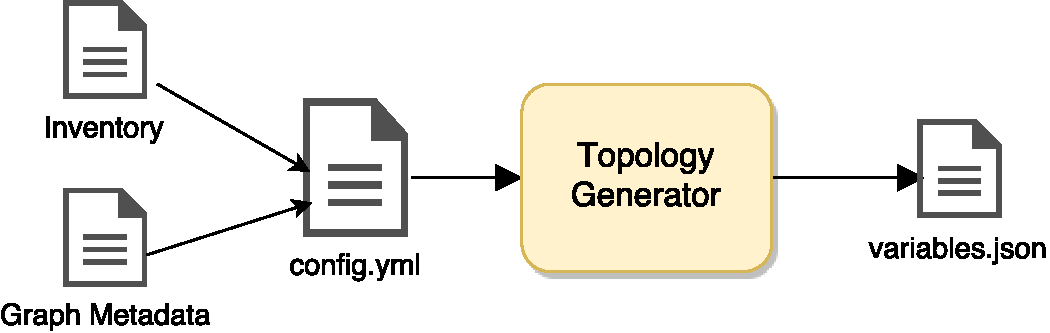
\includegraphics[width=10cm]{obrazky-figures/generator.pdf}
  \caption{Input and output scheme of the Topology Generator.}
  \label{fig:generator}
\end{figure}

\footnotetext{YAML - \url{http://docs.ansible.com/ansible/latest/YAMLSyntax.html}}

\subsection{Graph Metadata}
\label{Graph Metadata}
The technology which will be used for the actual implementation of Topology Generator is \emph{NetworkX}, a Python package for creation and manipulation of complex networks. This package offers features for creating graphs, multigraphs, random graph generators, plot created graph, and many more. NetworkX also offers graph import and export in YAML structured file, which is useful as graph metadata; simple example of this file is shown in Appendix \ref{AP:Graph Metadata}.

In this metadata user can specify any setting for each node. For example, user can specify the listener for router\,1, or connector for router\,2 as you can see in the example below.

\begin{verbatim}
---
directed: false
graph: {}
nodes:
- type: router
  id: router1
  listener:
  	- host: 0.0.0.0
  	  port: 1080
  	  role: inter-router
- type: router
  id: router2
  connector:
  	- name: router1
  	  host: router1
  	  port: 5675
  	  role: inter-router
multigraph: false
\end{verbatim}
From this metadata NetworkX creates two nodes with type, id, and listener or connector attributes. These attributes will be used to generates configuration files for each node. All possible attributes that user can specify for each node are available in Appendix \ref{AP:Qpid-Dispatch Configuration File Template}.

However, specifying all attributes of each node is not very user-friendly approach, especially in case of large topologies. So user can only specify nodes, and links between them and generator will add all necessary attributes in order to establish connection between nodes. The example of this metadata file can be seen in Appendix \ref{AP:Graph Metadata}.

\subsection{Topology Deployment}
Every node specified in the Inventory has to receive proper configuration files for services running on it. This job is handled by the Ansible, since it can connect to all nodes from Inventory and copy configuration files to proper destination folders. Ansible script load data from Topology Generator and creates configuration files based on loaded variables and the common template for Qpid-Dispatch. The created file will then be sent to the proper node based on node name from Inventory, which has to be same like router name specified in generated variables. The scheme of configuration deployment is depicted in the Figure \ref{fig:deployment}.

\begin{figure}[H]
  \centering
  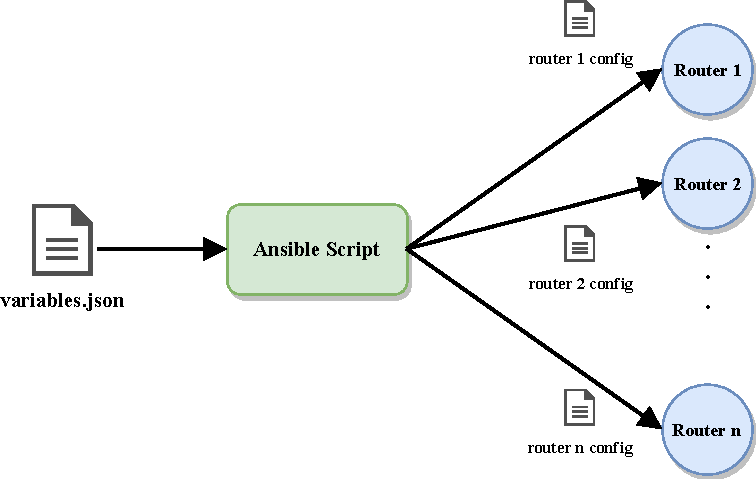
\includegraphics[width=12cm]{obrazky-figures/deployment.pdf}
  \caption{The scheme of configuration files deployment to the nodes.}
  \label{fig:deployment}
\end{figure}


\section{Qpid-Dispatch Agent Performance Module}
The architecture of Maestro (as depicted in the Figure \ref{fig:msg_perf_tool}) cannot use all performance testing and network recovery possibilities of the Qpid-Dispatch. For better performance analysis and measurements it is necessary to design and implement additional functionality for MPT.

In the Figure \ref{fig:msg_perf_tool_update} we show updated version of Maestro architecture. Proper performance testing of router and network analysis with few routers needs some kind of an agent, which can manipulate each node. In particular, MPT should be able to shut down one of the router node and collect data about network behavior during this situation. All these actions will be handled by the new back-end component called \emph{Agent}.

\begin{figure}[H]
  \centering
  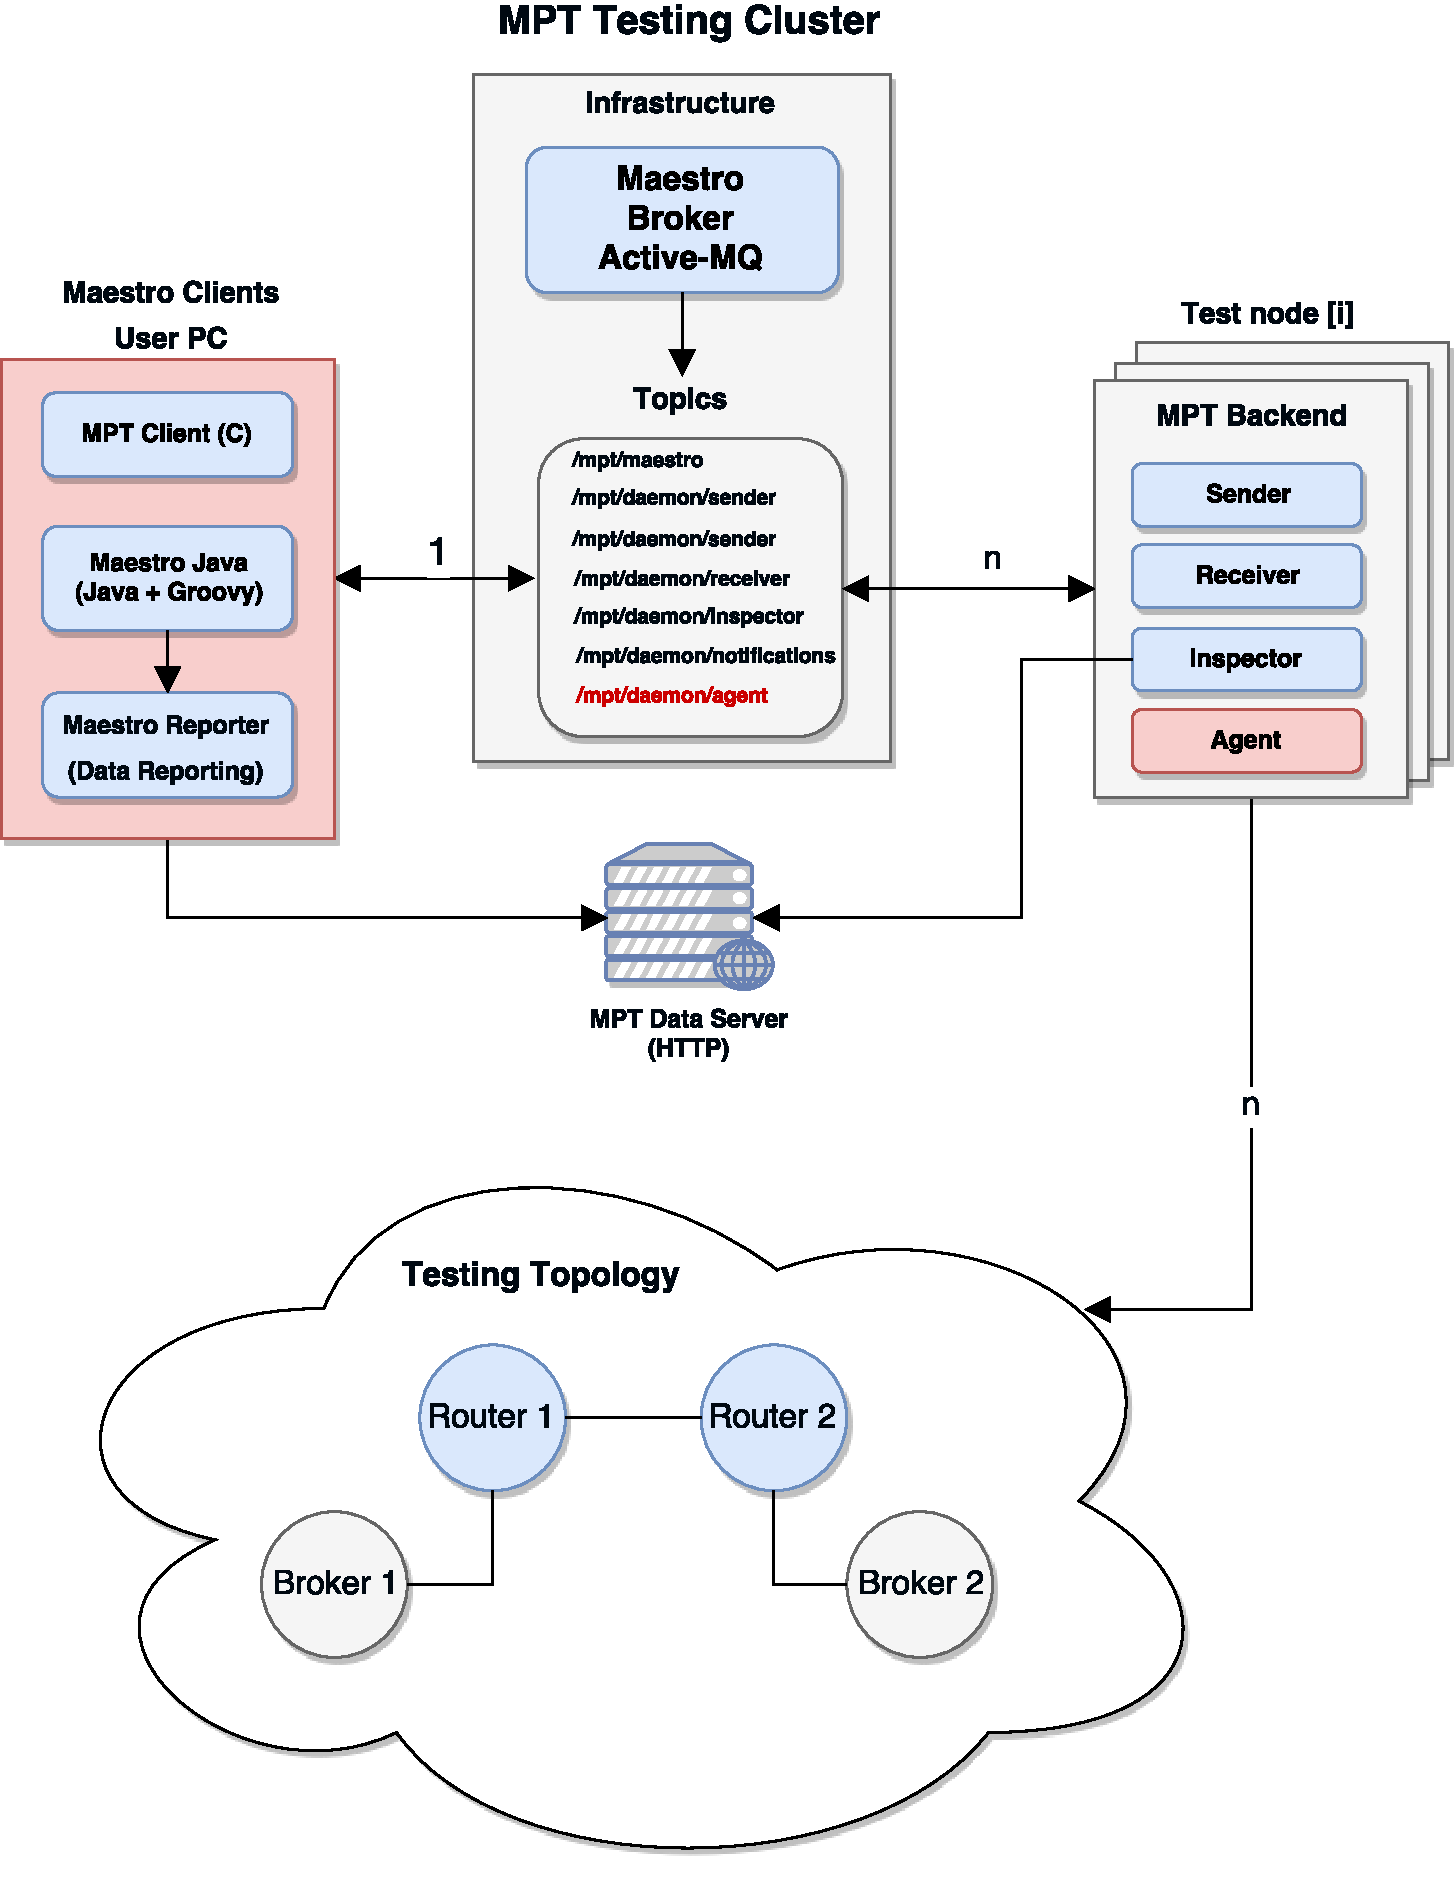
\includegraphics[width=15cm]{obrazky-figures/msg_perf_tool_for_router.pdf}
  \caption{The architecture of updated Maestro for testing of the Qpid-dispatch router.}
  \label{fig:msg_perf_tool_update}
\end{figure}

In the Figure \ref{fig:agent_1} we show the simple scheme of topology and one agent monitoring the router\,2. Communication passes through the router\,2 and messages are delivered to receiver without problems. The Figure \ref{fig:agent_2} demonstrates the shutdown of router\,2  by the agent. In that case, the network will choose the redundant link through router\,3 in order to pass messages. This scenario can answer the question \emph{How does this incident influence the latency between sender and receiver?}

\begin{figure}[H]
	\centering
	\begin{minipage}{6.5 cm}
		\subfloat[Network with router agent.\label{fig:agent_1}]{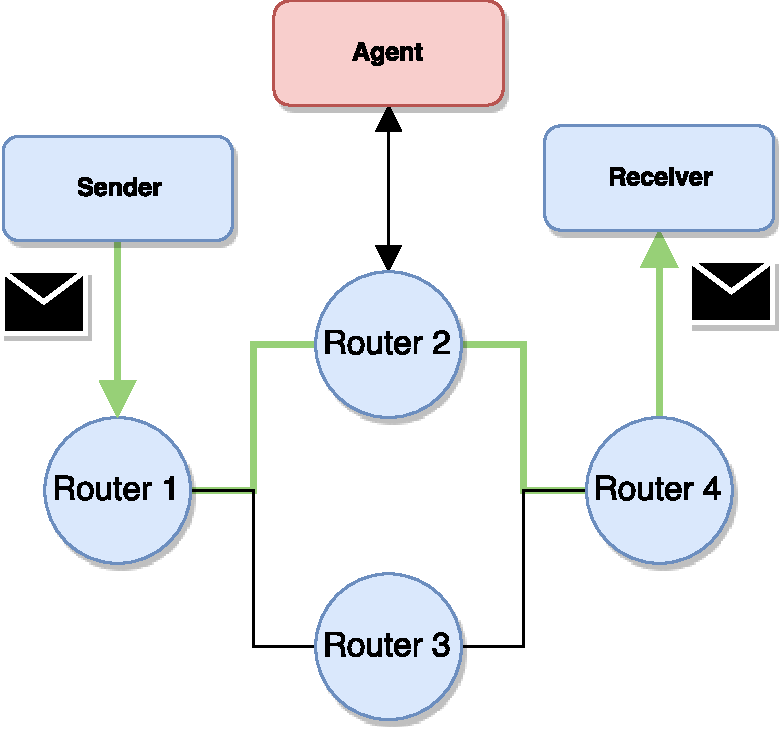
\includegraphics[width=1\linewidth]{obrazky-figures/agent_1.pdf}}
	\end{minipage}
	\begin{minipage}{6.5 cm}
		\subfloat[Router shut-down demonstration.\label{fig:agent_2}]{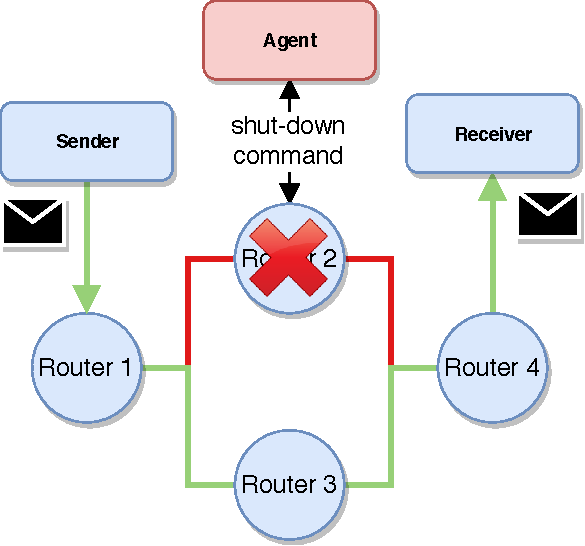
\includegraphics[width=1\linewidth]{obrazky-figures/agent_2.pdf}}
	\end{minipage}
	\caption[A simple network with active router agent.]{Simple network with router shut-down demonstration.}\label{fig:agent}
\end{figure}

Another part is a communication inside Maestro cluster with new component. Communication between cluster back-end and user client is realized through Maestro Broker and for proper message distribution new topic has to be added. As was mentioned in Section \ref{Collected Data Format}, Maestro Clients communicates with back-end via specialized commands. Router Agent will accept new set of commands for router control. This set has to be added to existing Maestro Clients. All additional components or components for update are highlighted by red color in the Figure \ref{fig:msg_perf_tool_update}. The example of simple testing topology consisting of two routers and two brokers is also included in the Figure \ref{fig:msg_perf_tool_update}.


\subsection{Extension Points}
\label{Extension Points}
After research and few discussions we decided to develop the agent as a service with dynamic command execution, which is able to run any specific code. At the begging of the test, the agent will receive the command for download some repository with specific scrips as a action handlers. The path to repository will be a payload of one of the new commands. After that, the agent will listen on the Maestro Broker topic for the agents and wait for user's command to execute. This command will transport the name of the handler script as a payload of the Maestro note. The agent will execute script from payload as an action on the node. In particular, the router restart handler can be part of downloaded repository and then can be performed after receive user commands with payload \emph{\"requests/router\_restart.groovy\"}. This functionality makes the agent dynamic, which offers to user execute any specific action what he wants.


\subsection{Communication with Agent}
\label{Communication with Agent}
For the communication inside Maestro testing cluster the Maestro Protocol is used which was described in the Subsection \ref{Communication Between Components}. MPT Clients have to know how to communicate with this new component in the cluster and for this it is necessary to add new communication commands. The following list shows new commands which should be added:

\begin{itemize}
	\setlength\itemsep{0em}
	\item \textbf{MAESTRO\_NOTE\_START\_AGENT (18)}\,---\,start the agent service.
	\item \textbf{MAESTRO\_NOTE\_STOP\_AGENT (19)}\,---\,stop the agent service.
	\item \textbf{MAESTRO\_NOTE\_AGENT\_SOURCE (21)}\,---\,path to user commands handlers.
	\item \textbf{MAESTRO\_NOTE\_USER\_COMMAND (30)}\,---\,user's specific command.
\end{itemize}

\subsection{AMQP Inspector}
\label{AMQP Inspector}
The important part of performance testing is measurements of internal metrics of SUT. Maestro offers Maestro inspector for this kind of measurements. However, current version can monitor only Broker, because Inspector is implemented for specific interface which is provided by Broker. Since Broker is written in Java and provides access to JMX\footnote{JMX\,---\,\url{http://www.oracle.com/technetwork/articles/java/javamanagement-140525.html}} via Jolokia\footnote{Jolokia\,---\,\url{https://jolokia.org/}}, we cannot use current Inspector for router as well. The router offers \emph{AMQP management} for interaction with the router on the fly, which is different than Jolokia access. The Jolokia access is based on HTTP/JSON format message exchange between requester and SUT. AMQP Management is based on AMQP messages with specific format.

The router offers these information after proper AMQP request to an opened up listener with specific properties:

\begin{itemize}
	\setlength\itemsep{0em}
		\item \textbf{name}\,---\,this property is always setup to \textbf{self}.
		\item \textbf{operation}\,---\,AMQP management offers classic CRUD operations. For inspect message we will always use option called \textbf{QUERY}.
		\item \textbf{type}\,---\,this property represents interior package which will parse the request, we will use \textbf{org.amqp.management}.
		\item \textbf{entityType}\,---\,this property is configurable. We use there several options with prefix \textbf{org.apache.qpid.dispatch.} based on request purpose. The options are:
		\begin{itemize}
			\setlength\itemsep{0em}
			\item \emph{router}\,---\,general informations about the router.
			\item \emph{router.stats}\,---\,detailed informations about the router.
			\item \emph{router.link}\,---\,informations about the route links.
			\item \emph{router.node}\,---\,general informations about neighbour nodes.
			\item \emph{router.address}\,---\,informations about addresses on the router.r
			\item \emph{connector}\,---\,informations about connections.
			\item \emph{allocator}\,---\,informations about memory metrics.
			\item \emph{config.autolink}\,---\,informations about created auto links.
			\item \emph{config.linkRoute}\,---\,informations about created link routes.
		\end{itemize}
		\item \textbf{body}\,---\,this property is message payload, which is empty list. Exceptions are auto links and link routes requests, which needs additional information in the body.
\end{itemize}

\subsubsection*{Collected Data}
\label{Collected Data}
Data collected by the AMQP Inspector is different than collect current version of Inspector. After the discussion, we decided to collect data about \emph{general statistics}, \emph{router links} and \emph{memory}. Note, that each data set has multiple data columns, which are all available in Appendix \ref{AMQP Inspector Data Sets}. The following describes the most important data collected by the AMQP Inspector:

\begin{itemize}
	\setlength\itemsep{0em}
	\item \textbf{Timestamp}\,---\,the date and time for the data sample in the format YYYY-MM-DD hh:mm:ss using the W3C defined standard for datetime.
	\item \textbf{General Statistics}\,---\,basic informations about the router such as active connections, addresses, auto links, accepted messages and so on.
	\begin{itemize}
		\setlength\itemsep{0em}
		\item \textbf{Address Count}\,---\,activate addresses at current time.
		\item \textbf{Connections Count}\,---\,active connections at current time.
	\end{itemize}
	\item \textbf{Router Links}\,---\,informations about all router links which were opened to the router.
	\begin{itemize}
		\setlength\itemsep{0em}
		\item \textbf{Accepted Message Count}\,---\,accepted messages at current time.
		\item \textbf{Delivered Message Count}\,---\,delivered messages at current time.
		\item \textbf{Released Message Count}\,---\,released messages at current time.
		\item \textbf{Undelivered Message Count}\,---\,undelivered messages at current time.
	\end{itemize}
	\item \textbf{Memory Statistics}\,---\,informations about allocated memory by the router.
	\begin{itemize}
		\setlength\itemsep{0em}
		\item \textbf{Total Allocated Memory}\,---\,total allocated memory.
		\item \textbf{Memory Allocated by Threads}\,---\,total memory allocated by threads.
	\end{itemize}
\end{itemize}

Each data set is converted to chart, which represents collected values for each request. Data collected by senders and receivers remains the same as in the current version of MPT.

\section{Used Technologies}
Messaging Performance Tool is a project with several parts. The most of MPT, such as command parsing, reporting, clients abstractions and so on, is written in Java language. But whole MPT is not pure Java code. To specify a test, Groovy is used. Groovy is basically lightweight version of Java with several advantages. From my point of view Groovy scripts are more readable for those who are not much familiar with Java code. Groovy scrips are also used as reaction for specific commands for extension points, but this is deeply described in the Subsection \ref{MPT Preparations}.

On the other hand, Topology Generator is a new simple project. For easy integration to another projects, quick development, and easy code preview I developed it in \emph{Python} language. Whole generator is created as one package, which is available for installation on any machine with installed Python version 2.7 and higher. Already mentioned technologies are very common and almost every programmer have heard about Java and Python. In the following subsections I describe not common and well known technologies.

\subsection{Ansible}
Ansible \cite{Ansible} is simple automation framework which allow users to automate daily tasks on multiple nodes or containers. Basic types of tasks which can be automated by Ansible are:

\begin{itemize}
	\item \textbf{Provisioning}\,---\,setups the various servers user needs in the network infrastructure.
	\item \textbf{Configuration management}\,---\,changes configuration of an application, operation system or device. Basically this allows starting, stopping and restarting services, installing or updating applications or performing a wide variety of other configuration tasks.
	\item \textbf{Application deployment}\,---\,automatically deploys the internally developed application to specified systems with all dependencies.
\end{itemize}

Ansible scripts, called playbooks, are written in YAML language. This makes Ansible scripts easy to read for humans and simple to manage. Another advantage is that the user does not even need to know commands used to accomplish a particular tasks. All that is needed is to specify what state does user wants the system to be in. Ansible is available on multiple systems with really short list of dependencies; Linux based systems requires Python installed and Windows needs PowerShell; both systems requires SSH. Moreover, Ansible playbooks can be grouped together and create more complex scripts called roles. They are open-source and available in public repository.

\begin{figure}[H]
  \centering
  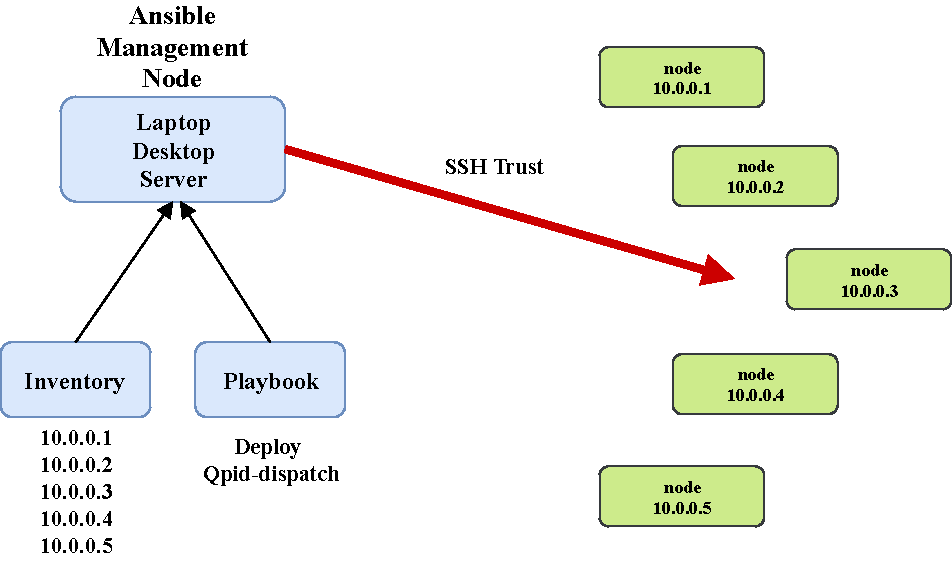
\includegraphics[width=12cm]{obrazky-figures/ansible_architecture.pdf}
  \caption{Ansible architecture witch several nodes. Inventory and Playbook are passed to Ansible Management node, which execute playbook on all node specified in the inventory.}
  \label{fig:ansible_architecture}
\end{figure}

We use Ansible used for several tasks; mainly to deploy systems on specific nodes. As I want to run performance tests of Qpid-dispatch over multiple topology scenarios it is necessary to do system deployment quickly and automatically, which is easy with Ansible. System deployment contains installation of MPT, Qpid-dispatch and other services based on testing scenario. The next task is to create and deploy configuration files for each router machine. This task runs Topology generator and creates configuration files for each machine based on generator output.


\subsection{Docker}
Docker \cite{Docker} is an open platform that provides developing, shipping, and running application separately from the infrastructure. Basically Docker is a specific type of virtualization technology. It allows to package and run an application in a loosely isolated environment called a container. These containers are lightweight virtual machines running directly within the host machine's kernel. This means that one can run more containers than virtual machines on specific hardware, and it is possible to run containers on virtual machines.

Docker container is build up from a dockerfile where container attributes are specified such as OS, environment variables, or steps for installing applications. Output of build command is then a docker image. This image is ready for running as a container with another specific attributes such as exposed ports. Containers can be attached to same network which allow communication between all containers.

\begin{figure}[H]
  \centering
  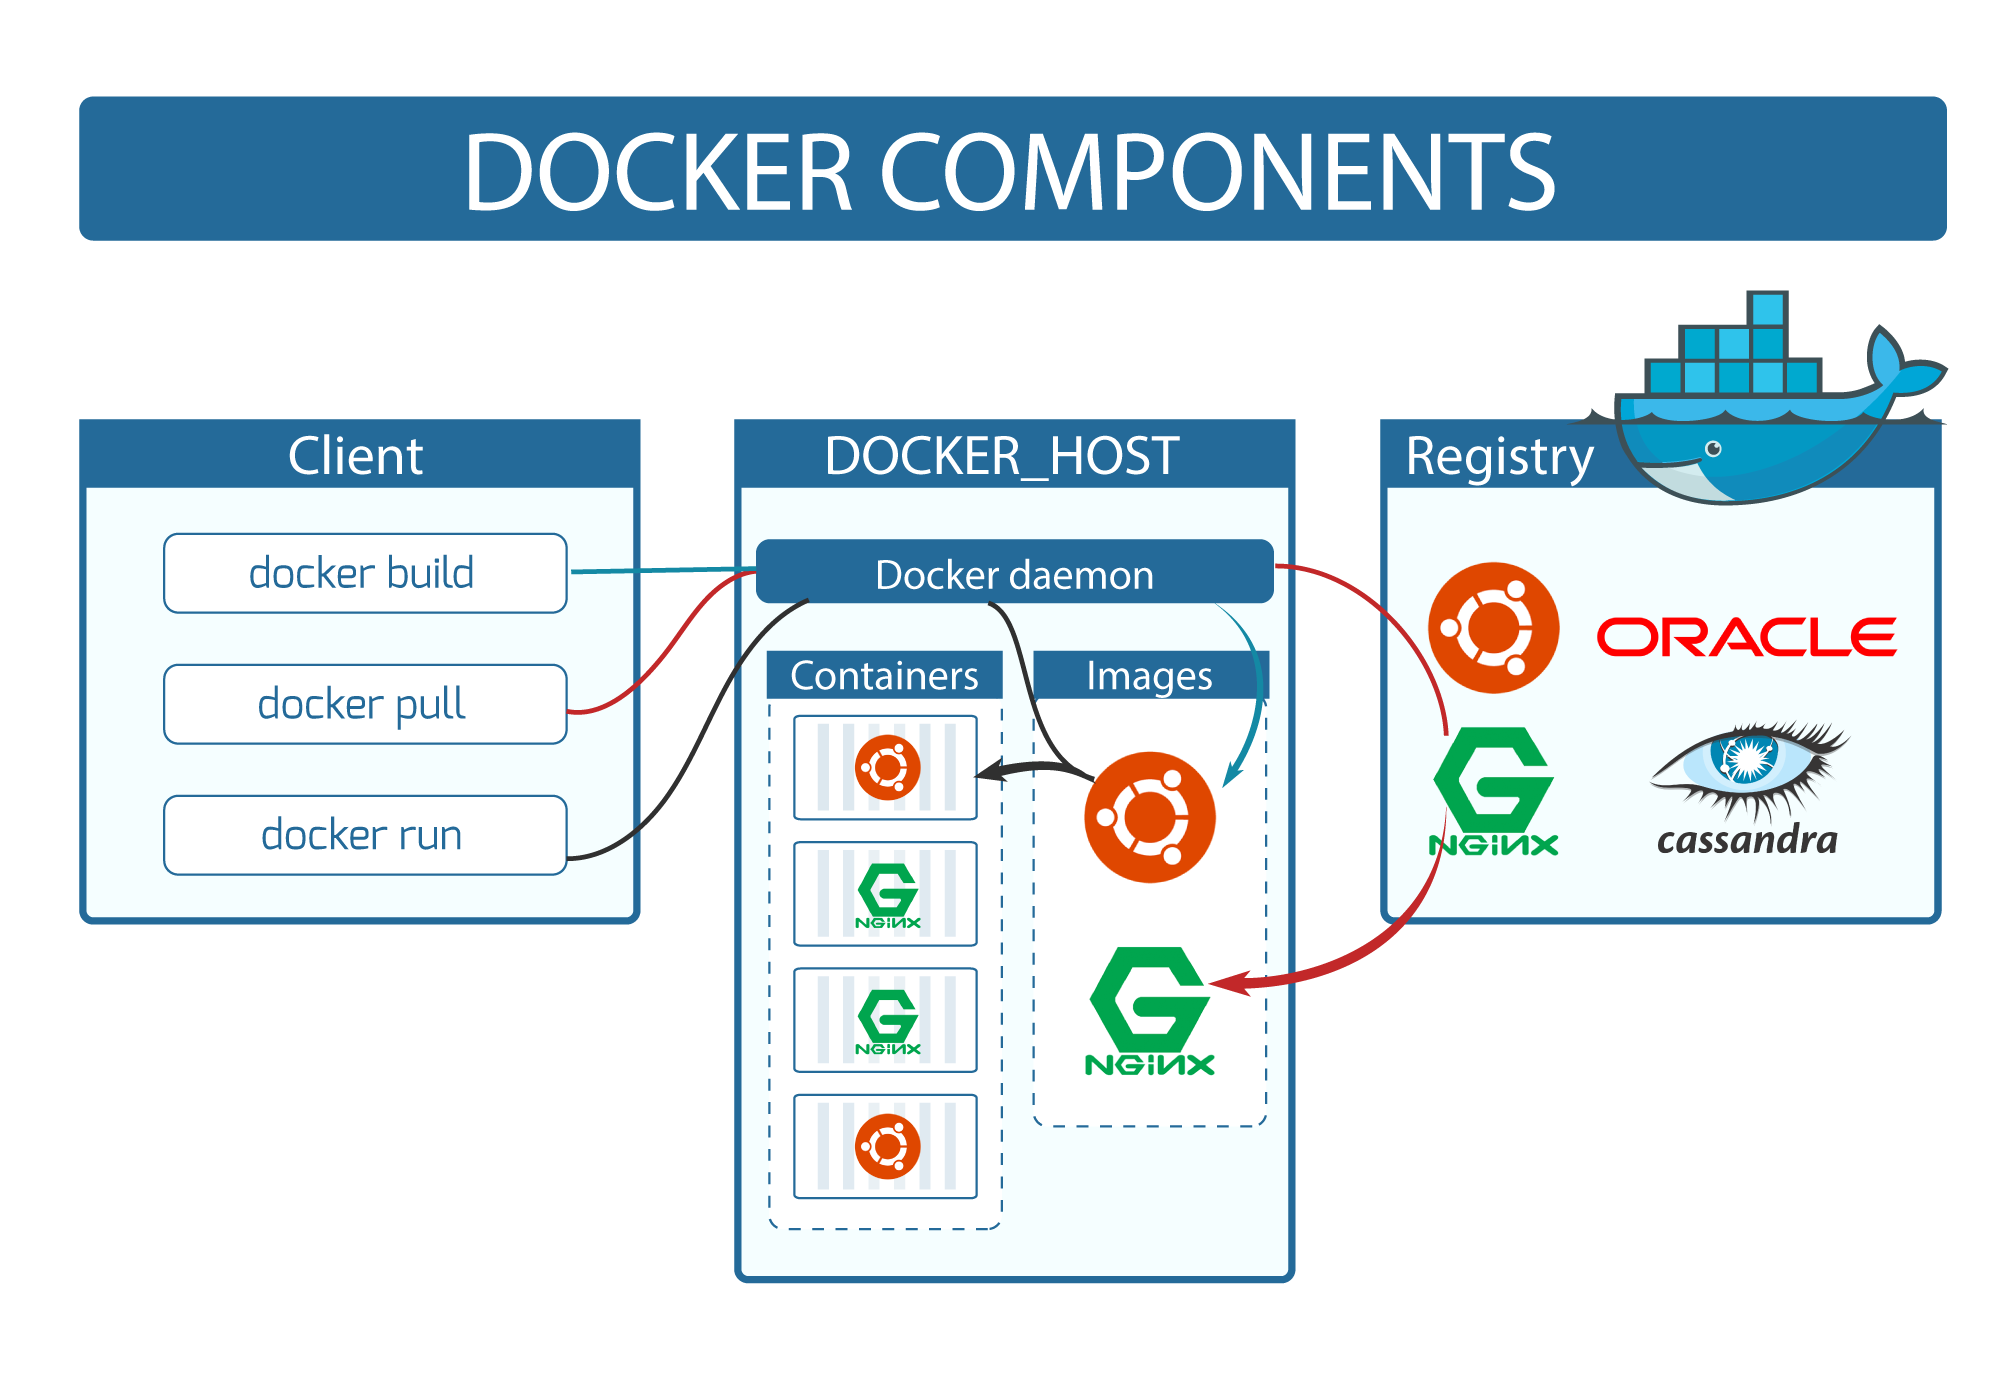
\includegraphics[width=13cm]{obrazky-figures/docker.png}
  \caption{Docker architecture with all its components and commands. Docker can pull or build specific image and then run it in docker container.}
  \label{fig:docker_architecture}
\end{figure}


Since docker is able to run services such as Qpid-dispatch very easily and also allow communication between containers. It is possible to deploy MPT with proper SUT in containers and analyze behavior in the container network or just run MPT on single machine. However, for proper performance results we need real machines, docker containers are used only for MPT development and trying some basic stuffs with MPT. The docker architecture is depicted in the Figure \ref{fig:docker_architecture}\footnote{Image is taken over from \url{https://robinsystems.com/blog/containers-deep-dive-lxc-vs-docker-comparison/}.}.

  % (c) Jakub Stejskal
% Master Thesis
% Performance Testing and Analysis of Qpid-Dispatch Router
% Chapter 5
\chapter{Implementation}
\label{Implementation}
This chapter describes the actual implementation details of all components, described in the Chapter \ref{Analysis and Design}. The main part focuses on the Agent module and AMQP Inspector for Maestro, which we implemented in Java and Groovy languages. The other part describes the Topology Generator\,---\,Python package for automatic generation of dispatched topology based on user's metadata. Data collecting and reporting done by Maestro parts has already been mentioned in the Chapter \ref{Analysis and Design}.

\section{Topology Generation}
Qpid-dispatch has a lot of configurable attributes, which can influence the router behavior. These attributes can be set up with an AMQP management tool called \emph{qdmanage}\footnote{qdmanage\,---\,\url{https://qpid.apache.org/releases/qpid-dispatch-1.0.1/man/qdmanage.html}} or one can specify them directly in the configuration file. However, qdmanage needs human interaction. It is more comfortable to create a configuration file for each specific test case. Hence, this initiated implementing of automatic Topology Generator.

In case of network with multiple routers, it is uncomfortable to update configuration files for each router on a specific node. Topology Generator introduces an option to update only a single file with router specifications and leave generation and deployment to an automated script. The actual generation takes few simple steps to achieve correct configuration files. These steps are used in Ansible script and are described in the following.

\subsection{Configuration File Generation}
It is important to note that each configuration file is not generated by Topology Generator itself, but by Ansible playbook. Why do we need such approach? Since Qpid-dispatch is getting new versions every few months, they can change names of any configuration attributes or even deprecate them. This causes the problem, that when Qpid-dispatch is updated, then the code of Topology Generator has to be reviewed and updated as well, otherwise one risks syntax errors in the configuration files. So such approach is not very stable, and hence the simple solution is to let Ansible do the final generation.

The trick is, that Ansible is able to fill-up any kind of passed \emph{Jinja2}\footnote{Jinja2\,---\,modern and designer-friendly templating language for Python \url{http://jinja.pocoo.org/docs/2.10/}} template only with data which are available. Basically, the Ansible playbook will get the configuration template and variables for router configuration files and create a proper configuration file. The script simply iterates through template and fills-up all available attributes. This process is repeated for every router machine in the Inventory file. Input configuration variables are in JSON format, and Ansible can recognize which variables are for particular machine.

\subsection{Template Generator}
Output configuration files are strictly based on input configuration template. This means that Ansible needs the input template with specific attributes for each version. However, Qpid-dispatch offers a solution how to construct this template. Attributes are available inside a JSON file in the installation folder of Qpid-dispatch. To process this JSON file and create resulting configuration template we use a tool called \emph{qdrouter-jinja2}\footnotemark{}.

\footnotetext{qdrouter-jinja2\,---\,\url{https://github.com/rh-messaging-qe/qdrouter-jinja2}}

Qpid-dispatch configuration file is divided into the multiple section where each sections has its own attributes. For example there is a \emph{router} section with router name, or mode, and \emph{ssl} section with security attributes. Each section can be specified multiple times, but usually only the last one found is used. The exceptions are \emph{connectors}, \emph{listeners}, \emph{addresses} and \emph{link routes} that can specify multiple connection points and routing types on single router. In the Algorithm \ref{alg:ansible_template_generator} you can see pseudo-code of template generation process.

\begin{center}
	\begin{algorithm}[H]
		\LinesNumbered
		\DontPrintSemicolon

		\SetKwFor{forPy}{for}{:}{}
		\SetKwIF{If}{ElseIf}{Else}{if}{:}{else if}{else}{}
		\SetKw{in}{in}
		\SetKw{var}{var}

		\KwIn{\emph{attributes\_file}\,---\,input file in JSON format}
		\KwOut{output file in Jinja2 format}
		\var output = ''''\;
		\forPy{line \in attributes\_file}{
			\If{line.is\_attribute()}{
				output += line.attributeToJinja2()
			}
			\uElseIf{line.is\_section()}{
				output += line.sectionToJinja2()
			}
			\Else{
				output += line
			}
		}
		output.strip()\;
		\KwRet{output}
		\caption{Template generation by qdrouter-jinja2.}
		\label{alg:ansible_template_generator}
	\end{algorithm}
\end{center}

From the pseudo-code you can see that there are two kind of wrappers for processing the JSON. Their function is to make configuration sections and attributes optional and repeatable which is achieved by wrapping the sections and attributes with Jinja2 code. The attribute wrappers processes each attribute line into the following template snippet:

\begin{verbatim}

    attribute: {{ section.attribute }}

\end{verbatim}

This code in template specifies, that if Ansible knows the variable \emph{section.attribute}, it will add a line with that attribute name and variable value into the configuration file. Key words section and attribute are just placeholders for real names such as \emph{connector} for section and \emph{host} for attribute. Output can then look like the following line:

\begin{verbatim}
		host: 10.0.0.1
\end{verbatim}

The section wrapper is more complex, because it has to wrap the start and the end of the section. This is handled by class methods \texttt{\textunderscore enter\textunderscore ()} and \texttt{\textunderscore exit\textunderscore ()} which allows you to implement objects that execute \texttt{\textunderscore enter\textunderscore ()} at start and \texttt{\textunderscore exit\textunderscore ()} at the end of some statement. Basically this class is dynamically created for each section and these methods are then invoked before first and after last attribute. The \texttt{\textunderscore enter\textunderscore ()} method wraps start of each section with following code:

\begin{verbatim}


section_name {
\end{verbatim}

The \textbf{\textunderscore exit\textunderscore ()} method closes the section with the following piece of code in the Jinja2 template:
\begin{verbatim}
}


\end{verbatim}

Since qdrouter-jinja2 parses JSON data from the installed version of Qpid-dispatch on remote node it guarantees that the template will always correspond with the specific router version. The template is saved in \emph{/tmp} folder on the remote machine where Ansible scripts can fetch it into the local folder and fill it up with data.

\subsection{Topology Generator}
Topology Generator is the main actor in configuration generation and deployment. It process configuration variables for Ansible deployment scripts from the user specification. Topology Generator requires two parameters: the path to the Inventory and the path to the graph file or topology type.

\begin{description}
	\item \textbf{Path to the Inventory}\,---\,Inventory is simple configuration file with list of nodes, connected to the network. Generator retrieves node names and types (i.e. router or broker) and use them during the generation of variables. The generator creates specific sections and attributes based on node and graph types. Since broker configurations are not generated by this tool, generator uses information only about specification of link routes to neighbours. Broker configuration is based on XML files, where user can specify Broker attributes. However, the future goal is to generate configuration for Broker as well.
	\item \textbf{Path to Graph file}\,---\,Graph file is a simple YAML file which specifies node distribution in the network. It contains at least node name and links to another nodes. Beside the name, user can easily specify for each node informations such as constructors, listeners, SSL profiles, etc. The whole file is loaded during the initialization and is processed with the Topology Generator.
	\item \textbf{Topology Type}\,---\,Topology generator can create topologies without graph file, but then it requires the network type that will be generated. For example the topology type can be a line which puts all nodes into one line and generates connections between them.
\end{description}

Inner representation of network is realized by Python library \emph{NetworkX}\footnote{NetworkX\,---\,\url{https://networkx.github.io/documentation/latest/}}. It creates a graph as an object and offers manipulation with its attributes which are objects of nodes and links. Topology Generator is able to store information about network configurations as attributes of these objects. During the graph initialization, the generator stores basic information about nodes such as the name and the type from inventory or some additional information from the graph file. Basic algorithm of topology generation is depicted in the Algorithm \ref{alg:default_connections}.

However, the generation of each configuration section is more complex and is slightly different for each section for connections to another nodes. The actual generation is split into two parts based on the user's arguments: the first is the generation of the default connections and the other is the generation of user specific sections from the metadata file.

\begin{description}
	\item \textbf{Default Connections}\,---\,default connections correspond to configuration for establishing connection between two devices in the network. To achieve this one has to configure listeners, connections, addresses and link routers (depending on the second machine) on each router. These sections can be easily automatically generated only with the minimal knowledge about the network. The default connections are generated automatically when user specifies only hosts and topology type. The generator takes neighbours of each machine. Generator's output in that case is a file with variables for fully functional connections between machines. During the generation from the graph file each node has attribute which specifies if user wants the default connections. The Algorithm \ref{alg:default_connections} captures the default generation process.

	\item \textbf{User Specific Sections}\,---\,these sections are not needed for the proper communication inside the network. An example can be SSL or auto-links settings. The generator loads data about these sections from graph file. Qpid-dispatch has a lot of settings, hence the generator does only the basic connectivity configuration without any specific settings if the user does not specify otherwise. You can see the user specific sections generation in the Algorithm \ref{alg:default_connections} as the part of the first \emph{for} statement. This generation part is done alongside with default connections generation.

\end{description}

Used algorithms are pretty straightforward. Since the generator is able to load IP addresses from the inventory there has to be a mechanism for automatic generation of proper port numbers for listeners and connectors. The problem is, that connectors of node X and listeners of directly connected node Y has to have same port numbers. It means, that node X connects to a specific port on node Y and node Y listens on that port. The initial port number is 5672, the default AMQP port, and it is incremented with each newly created listener. Hence, the listeners must be generated first on all nodes and then the connectors can be generated. This allows the access to port numbers of neighbor listeners via a simple method and explains the double loop over nodes in the Algorithm \ref{alg:default_connections}.

\begin{center}
	\begin{algorithm}[H]
		\LinesNumbered
		\DontPrintSemicolon

		\SetKwFor{forPy}{for}{:}{}
		\SetKwIF{If}{ElseIf}{Else}{if}{:}{else if}{else}{}
		\SetKw{in}{in}
		\SetKw{var}{var}

		\KwIn{Inventory, Graph File/Topology Type}
		\KwOut{output file in JSON format}
		\var inventory = parse\_inventory(Inventory)\;
		\var graph = create\_graph(inventory, Graph File/Topology type)\;
		\var output = \{\}\;
		\forPy{node, neighbors \in graph.adjacency()}{
			output.update(generate\_listeners(node, neighbors))\;
			output.update(generate\_addresses(node, neighbors))\;
			output.update(generate\_specific(node, neighbors))\;
		}

		\forPy{node, neighbors \in graph.adjacency()}{
			connectors, link\_routes = generate\_connectors(node, neighbors)\;
			output.update(connectors)\;
			output.update(link\_routes)\;
		}
		\KwRet{output}
		 \caption{Pseudocode of default connectivity generation.}
		 \label{alg:default_connections}
	\end{algorithm}
\end{center}

\begin{center}
	\begin{algorithm}[H]
		\LinesNumbered
		\DontPrintSemicolon

		\SetKwFor{forPy}{for}{:}{}
		\SetKwIF{If}{ElseIf}{Else}{if}{:}{else if}{else}{}
		\SetKw{in}{in}
		\SetKw{var}{var}
		\SetKw{fce}{Function: }

		\fce \emph{generate\_connectors()}\;
		\KwIn{\emph{node}---node from graph, \emph{neighbors}}
		\KwOut{lists of connectors and link\_routes}
		\var connectors = []\;
		\var link\_routes = []\;
		\forPy{neighbor \in neighbors}{
			\If{neighbor.is\_router()}{
				connectors.append(connector\_setting)\;
			}
			\uElseIf{neighbor.is\_broker()}{
				connectors.append(connector\_setting)\;
				link\_routes.append(link\_route\_setting)\;
			}
		}
		\KwRet{connectors, link\_routes}

		 \caption{Connectors and link routes generation. The algorithm describes function \texttt{generate\_connectors()}.}
		 \label{alg:link_routes}
	\end{algorithm}
\end{center}

The Algorithm \ref{alg:link_routes} shows the generation process of connectors and link routers. The connectors are generated for other network service (router/broker), but link routes are generated only in the case of the connection to the broker. The link route section then contains name or address of the connected broker, name of queue to which router will send the messages and specification of link route direction (input or output). For full-duplex connection to the broker one needs connector and two link routes from the router to the broker.

\subsection{Deployment}
At this point, everything is ready to create the Ansible playbook, to run all necessary tools and to deploy generated configuration files. Note, that each task can be executed on different machine based on the inventory.

The playbook combines all previously mentioned tools and also uses features from Ansible role \emph{ansible-qpid-dispatch}\footnote{Ansible-qpid-dispatch\,---\,Ansible role for install
and setup Qpid-dispatch. The role is available at \url{https://github.com/rh-messaging-qe/ansible-qpid-dispatch}} such as start and stop handlers. These steps can be added in any playbook or role, and can be used for automatic topology generation and deployment. The necessary inputs are Inventory and topology metadata for each test-case. In the following description you can see the list of all deployment steps, that are executed on the control node (node where we use the playbook):

\begin{description}
	\item \textbf{1. Install the Topology Generator}\,---\,Topology Generator is the main actor in the topology deployment so it is necessary to have it installed. Ansible takes care of it in the playbook.
	\item \textbf{2. Run the Topology Generator}\,---\,Topology Generator needs configuration files for proper execution. In the play one just needs to specify the path to configuration files and Ansible will do all other necessary steps.
	\item \textbf{3. Include variables into Ansible}\,---\,this step loads the generated variables into the memory. After this step, the script is ready to fill-up the template on remote machines.
\end{description}

Since Ansible offers smart system with variables inside the playbooks, one can assign all paths to configurations files to variable in the script or pass them with option during the playbook execution start. After these steps we are ready to execute the last steps on the remote nodes:

\begin{description}
	\item \textbf{4. Install qdrouter-jinja2} and \textbf{generate templates}\,---\,qdrouter-jinja2 is used to generate the template. We need to install it on all of router nodes, because each router can have different version and it can affect the configuration file with deprecated attributes. After the successful installation the templates are created.
	\item \textbf{5. Fill templates on remotes}\,---\,the script fills-up the template on each node. Since it has information about all nodes from configuration variables, it simply compares hostname with key from variables to assign proper data to each host.
	\item \textbf{6. Restart Qpid-dispatch}\,---\,after the change of configuration, we need to restart each machine and reload the configuration.
\end{description}

\section{Qpid-Dispatch Performance Module}
This section focuses on Maestro Agent implementation and necessary updates of all other Messaging Performance Tool parts such as commands updates, extension of the Inspector or report changes. The Agent was implemented in Java and Groovy languages.

\subsection{MPT Preparations}
\label{MPT Preparations}
The first step during the development was to update the Maestro project structure by adding the new module called \emph{maestro-agent}. The agent is designed as the new independent service, which can be run after the building of the package by Maven. At first, we need ti implement the main function for the agent, which is built with each new package. After the creation of main we had to create \emph{assembly.xml} which tells Maven which files has to be used for creation of new package during the build. The last step is to update all \emph{pom.xml} files, where are specified all dependencies and then we are ready to build and start the implementation.

\subsection{Agent Module}
As it was mentioned in Subsection \ref{Extension Points}, the agent is an independent service running on the testing node. Since Maestro already has a similar services, we can reuse the already working parts. The Maestro has a class \texttt{MaestroWorkerManager} which represents a simple Maestro peer. This class has a several important methods which are inherited and used by Agent as well:

\begin{itemize}
	\setlength\itemsep{0em}
	\item \texttt{connect()}\,---\,this method connects each peer to the Maestro Broker. Based on the peer function, it also subscribes the peer to all needed topics. For example, the sender peer does not need subscription to agent commands topic. When this method throws an exception, the peer was not able to connect to Maestro Broker and the test fails.
	\item \texttt{noteArrived()}\,---\,this method catches incoming notes from Maestro Broker and invokes action based on the note.
	\item \texttt{handle()}\,---\,this method handles each received note. We overload this method to invoke specific handler method based on the received note type. Usually, the \texttt{handle()} methods in \texttt{MaestroWorkerManager} class only logs actions. For another functionality we have overridden the specific implementations of each peer.
\end{itemize}

Every action handler script is written in Groovy, and so Maestro needed a Groovy script executioner. For this purpose, we created the class \texttt{GroovyHandler}. This class basically checks the handler file whether it is executable and then tries to execute it. The handler file location is specified by the note payload and there one can specify more than one file; \texttt{GroovyHandler} checks and execute all of the files.

The main part of the Agent is the method called \texttt{callbacksWrapper()}. Since the Agent overrides \texttt{handle()} method to execute scripts from external point, every \texttt{handle()} method in the agent calls the \texttt{callbacksWrapper()}. The basic functionality is shown in the Algorithm~\ref{alg:agent_note_handle}. The reason why \texttt{sendReplyOk()} is sent everytime is that we need to know if thread was started. For example we can start the thread with the command execution 5 minutes after the start. So we need the information if thread started successfully and then the information how the thread execution finished. However, the information about thread finish is sent by the handler itself. This is also reason why for every external point handler creates its own thread and naturally, the agent must serve other handlers during this time, and not wait 5 minutes for one of them to finish and then handle the others.

\begin{center}
	\begin{algorithm}[H]
		\LinesNumbered
		\DontPrintSemicolon

		\SetKwFor{forPy}{for}{:}{}
		\SetKwIF{If}{ElseIf}{Else}{if}{:}{else if}{else}{}
		\SetKwIF{try}{catch}{catch}{try}{}{catch}{catch}{}
		\SetKw{in}{in}
		\SetKw{var}{var}
		\SetKw{fce}{Function: }

		\fce callbacksWrapper()\;
		\KwIn{externalPointPath, codeDir, note}
		\KwOut{sendReplyOk() or sendReplyFail()}

		\var thread = Thread()\;

		\etry{}{
			\var groovyHandler = GroovyHandler()\;
			groovyHandler.setInitialPath(externalPointPath)\;
			groovyHandler.setWorkerOptions(getWorkerOptions())\;
			groovyHandler.setMaestroNote(note)\;
			thread.start(groovyHandler.runCallbacks())\;
		}{
			sendReplyFail()\;
		}

		sendReplyOk()\;

		 \caption{Basic functionality of \texttt{callbacksWrapper()} method. This method create new thread for each extension point and tries to execute it.}
		 \label{alg:agent_note_handle}
	\end{algorithm}
\end{center}

In new threads we execute \texttt{runCallbacks()} method, which load all files from extension point directory and tries to execute them. This method is in a specific class, which contains parameters for each execution. The parameters are originally contained in the note's payload. The Algorithm \ref{alg:agent_run_callbacks} captures \texttt{runCallbacks()} method.

\begin{center}
	\begin{algorithm}[H]
		\LinesNumbered
		\DontPrintSemicolon

		\SetKwFor{forPy}{for}{:}{}
		\SetKwIF{If}{ElseIf}{Else}{if}{:}{else if}{else}{}
		\SetKwIF{try}{catch}{catch}{try}{}{catch}{catch}{}
		\SetKw{in}{in}
		\SetKw{var}{var}
		\SetKw{fce}{Function: }

		\fce runCallbacks()\;
		\KwIn{groovyHandler as this class}
		\KwOut{sendReplyOk() or sendReplyFail()}

		\forPy{file in extensionPointDirectory}{
				\etry{}{
						\var grovyObject = loadFileAsGroovyObject(file)\;
						groovyObject.invokeMethod(”setMaestroNote”, this.maestroNote)\;
						groovyObject.invokeMethod(”setWorkerOptions”, this.workerOptions)\;
						groovyObject.invokeMethod(”setMaestroClient”, this.client)\;
						groovyObject.invokeMethod(”handle”, this.context)\;
				}{
						sendReplyFail()\;
				}
		}

		sendReplyOk()\;

		 \caption{The method \texttt{runCallbacks()} loops over each file in the extension point directory, tries to load each file and executes it.}
		 \label{alg:agent_run_callbacks}
	\end{algorithm}
\end{center}

The other important method of Agent is the override \texttt{handle()} for \emph{AgentSourceRequest} note. After this note is received, the \texttt{handle()} method fetches a git repository URL from the note and tries to clone it. The current version offers to clone any public git repository and even the specific branch of the repository.

\subsubsection*{Agent Capabilities}
\label{Agent Capabilities}
The current implemented version of the Agent offers much more features than was originally designed. The Agent does not focus only on Qpid-dispatch actions handling, but it can invoke action on node itself by executing extension points scripts. This makes agent usable also for Broker nodes, where it can simulate a real network behavior during the testing. The agent can also run third party software on the node during the test, which can simulate any kind of  the unexpected behavior.

The agent is a specific kind of Maestro Worker. This means, that agent connected to the Maestro Broker can publish messages during the test about its execution status or any additional information. You can see a simple communication with agent notes handling in the Figure \ref{fig:agent_demo}. The notes are send from the front-end through the Maestro Broker. Agent then invokes a specific handle method based on the received note. Inspector keeps inspecting the Qpid-dispatch by requests about his state every 15\,seconds.

\begin{figure}[H]
  \centering
  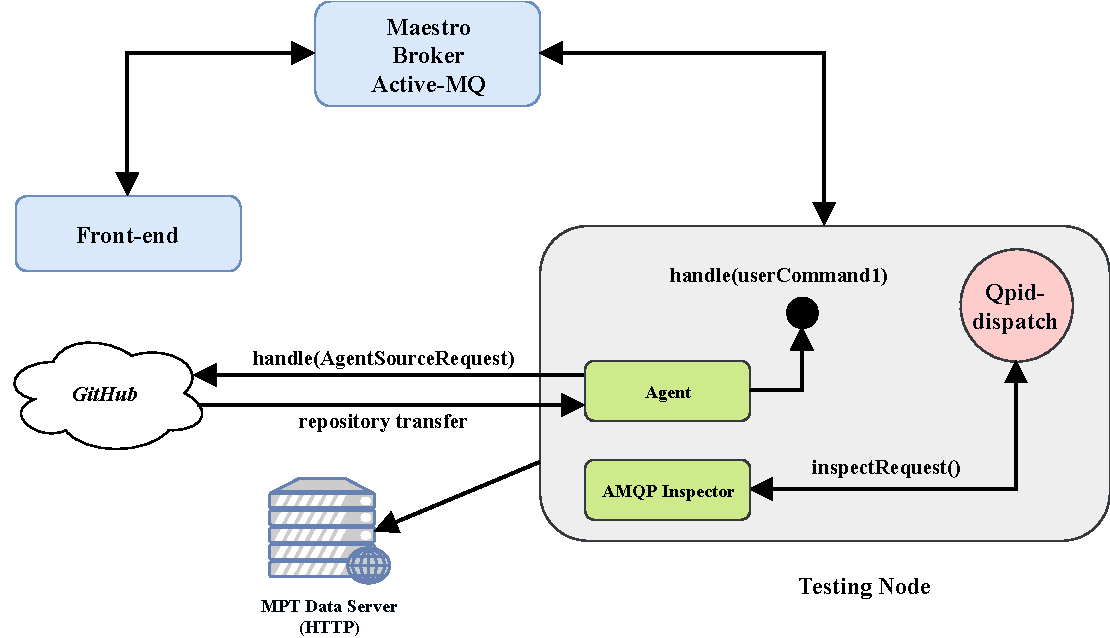
\includegraphics[width=15cm]{obrazky-figures/agent_demo.pdf}
  \caption{Communication scheme inside the Maestro with the agent. Scheme shows the agent git repository download and then handling the proper note defined by the user. The Figure also shown the SUT communication with the AMQP Inspector.}
  \label{fig:agent_demo}
\end{figure}

\subsection{AMQP Management Inspector}
\label{AMQP Management Inspector}
The collection of information about the router itself is not gathered by the agent. For this purpose, we developed a new type of Maestro Inspector specific for AMQP Management. AMQP Management is layered on top of the AMQP protocol and it access the inner data about the router by a simple requests and responses. Qdmanage tool already has implemented operations for AMQP Management, however, qdmanage is a Python tool and we want to integrate only Java code with AMQP Management requests into the Maestro. While AMQP Management offers CRUD operations for router configuration and inter informations, for AMQP Inspector we are fine with only Read operation to get specific information about running the instance of Qpid-dispatch.

\subsubsection*{Basic Evaluation}
The Maestro Inspector is designed to run a specific Inspector class based on user definition in the testing script. Currently, Maestro offers ActiveMQ Inspector for the Broker and AMQP Inspector for the Router. The Inspector will receive the note with \emph{inspector start} command, which carries string payload. This payload is the name of the specific inspector implementation that will be started. The mechanism of starting the AMQP Inspector is depicted in the Figure \ref{fig:inspector_start} and in the Algorithms \ref{alg:startInspector}.

\begin{figure}[H]
  \centering
  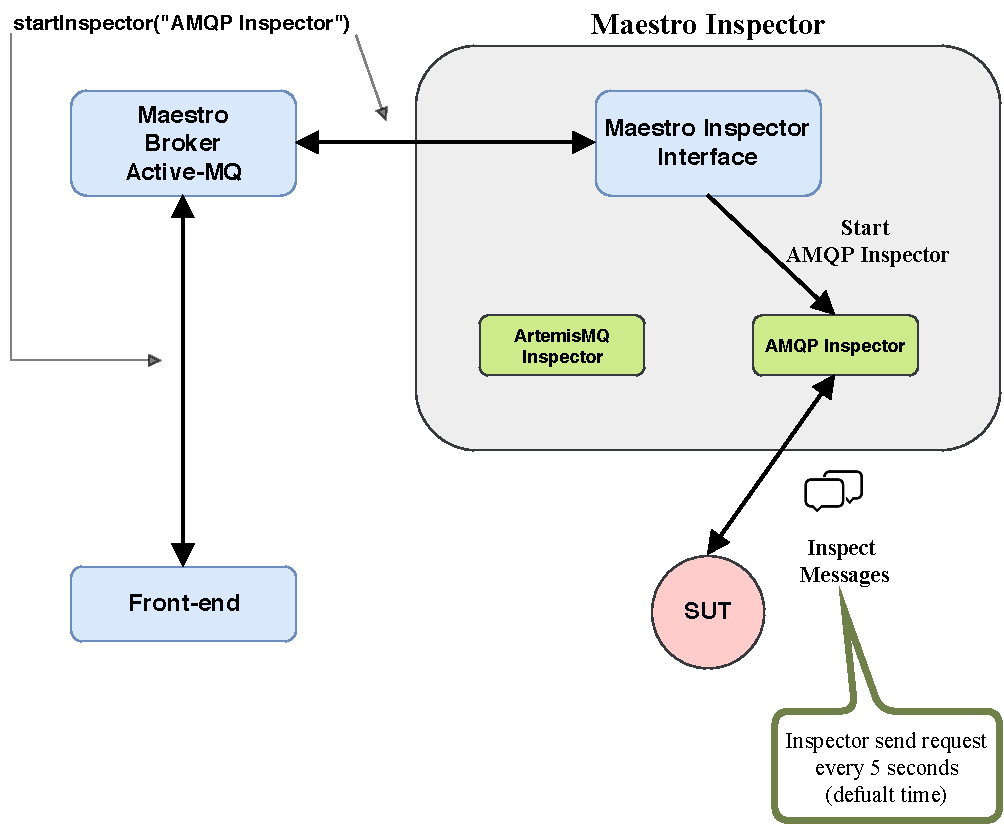
\includegraphics[width=13cm]{obrazky-figures/inspector_start.pdf}
  \caption{The inner mechanism of Maestro Inspector during the receive start inspector note. One can see the note exchange and choose of specific inspector class based on the note's payload.}
  \label{fig:inspector_start}
\end{figure}

\begin{center}
	\begin{algorithm}[H]
		\LinesNumbered
		\DontPrintSemicolon

		\SetKwFor{forPy}{for}{:}{}
		\SetKwIF{If}{ElseIf}{Else}{if}{:}{else if}{else}{}
		\SetKwIF{try}{catch}{catch}{try}{}{catch}{catch}{}
		\SetKw{in}{in}
		\SetKw{var}{var}
		\SetKw{fce}{Function: }

		\fce \emph{handle()}\;
		\KwIn{Maestro note\,---\,startInspector}
		\KwOut{sendReplyOk() or sendReplyFail()}

		\var inspectorClass = note.getPayload()\;

		\etry{}{
			\var inspector = Inspector(inspectorClass)\;
			\var thread = Thread(inspector)\;
			thread.start()
			sendReplyOk()\;
		}{
			sendReplyFail()\;
		}

		 \caption{Handler method for startInspector note which creates instance of specific inspector implementation.}
		 \label{alg:startInspector}
	\end{algorithm}
\end{center}

\begin{center}
	\begin{algorithm}[H]
		\LinesNumbered
		\DontPrintSemicolon

		\SetKwFor{forPy}{for}{:}{}
		\SetKwFor{whilePy}{while}{:}{}
		\SetKwIF{If}{ElseIf}{Else}{if}{:}{else if}{else}{}
		\SetKwIF{try}{catch}{catch}{try}{}{catch}{catch}{}
		\SetKw{in}{in}
		\SetKw{var}{var}
		\SetKw{fce}{Function: }

		\fce \emph{start()}\;
		\KwOut{sendReplyOk() or sendReplyFail()}

		\var routerLinkInforWriter = RouteLinkInfoWriter()\;
		\var memoryInfoWriter = MemoryInfoWriter()\;
		\var generalInfoWriter = GeneralInfoWriter()\;

		\etry{}{
			\var currentTime = System.currentTimeMillis()\;
			connectToRouter()\;
			\var dataReader = DataReader()\;

			\whilePy{canContinue()}{
				 routerLinkInforWriter.write(currentTime, dataReader.collectRouterInfo())\;
				 memoryInfoWriter.write(currentTime, dataReader.collectMemoryInfo())\;
				 generalInfoWriter.write(currentTime, dataReader.collectGeneralInfo())\;

				Thread.sleep(5000)
			}
			sendReplyOk()\;
		}{
			sendReplyFail()\;
		}

		 \caption{Method for starting new instance of the Inspector. This method continuously sends requests to the SUT, collects, parse and write the response into csv file.}
		 \label{alg:requester}
	\end{algorithm}
\end{center}

\begin{figure}[H]
  \centering
  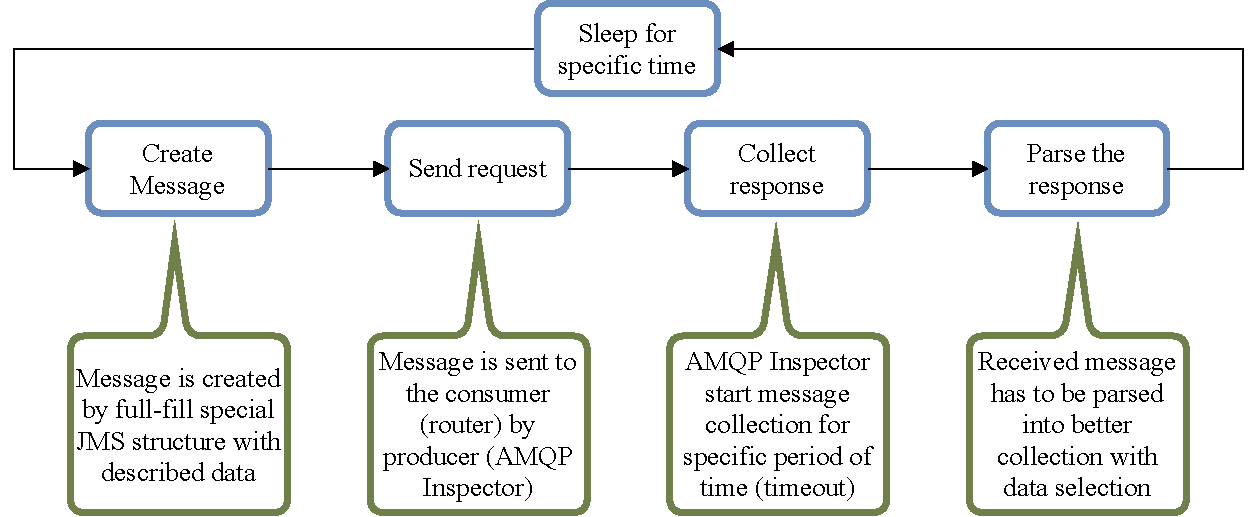
\includegraphics[width=12.5cm]{obrazky-figures/inspector_collector.pdf}
  \caption{The whole Inspector process including message creation, message sending, collecting and parse.}
  \label{fig:collector}
\end{figure}


The AMQP Inspector uses the request-response message mechanism with the SUT. The inspector creates message using Java library \emph{Qpid JMS}\footnote{Qpid JMS\,---\,\url{https://qpid.apache.org/components/jms/index.html}} as specified in the Subsection \ref{AMQP Inspector}. Since we want to collect as much relevant data as possible, we are sending three\footnote{Three specific requests to AMQP Management are enough to collect all data which are needed.} request-response messages with different \texttt{entityType} option every 5\,seconds during the whole test. For the response collecting it is necessary to create a temporary queue, that is used by the router as response destination. The destination is contained in the field \emph{response-to}. The actual request message is represented as an object with type of \emph{JMS Message}. The main Inspector's process mechanism is described in the Algorithm \ref{alg:requester}, while the message request-response mechanism is depicted in the Figure \ref{fig:collector}.

  % (c) Jakub Stejskal
% Master Thesis
% Performance Testing and Analysis of Qpid-Dispatch Router
% Chapter 6

\chapter{Experimental Evaluation}
\label{Experimental Evaluation}
This chapter summarizes results of the performance testing and experimental evaluation with Maestro. We split the experiments into two parts. The first performs a basic measurement of Maestro\,1.3.0 which includes Maestro Agent and AMQP Inspector. During this measurements we focused on the highest possible throughput of singlepoint topology of Qpid-dispatch and Message Broker and multipoint topologies with three nodes of Qpid-dispatch and with Broker in the middle. The experimental topologies are depicted in the Figure \ref{fig:basic_topologies}. The later series of experiments focused on behavior testing of the topologies, which involves Qpid-Dispatch reliability and recovery testing.

Since the testing was executed over multiple topology types, we used Topology Generator for quick automatic changes of topology. Each test was executed against established topology where all components was newly installed and restarted between each test scenario. This was done during the cleaning stage. For experimental evaluation we used machines specified in the Table \ref{tab:machines}. The reason why the clients uses powerful machines is that we need more machines for SUT, but only two IBM Xeon machines was available during the experimental evaluation and we need at laest three machines for the SUT nodes.

% Please add the following required packages to your document preamble:
% \usepackage[table,xcdraw]{xcolor}
% If you use beamer only pass "xcolor=table" option, i.e. \documentclass[xcolor=table]{beamer}
\begin{table}[]
\centering
\caption{Machines and their properties, which were used for the experimental evaluation.}
\label{tab:machines}
\begin{tabular}{|l|l|r|r|}
\hline
\rowcolor[HTML]{C5E3DF}
\textbf{} & \multicolumn{1}{c|}{\cellcolor[HTML]{C5E3DF}\textbf{Machine}} & \multicolumn{1}{c|}{\cellcolor[HTML]{C5E3DF}\textbf{CPU}} & \multicolumn{1}{c|}{\cellcolor[HTML]{C5E3DF}\textbf{RAM (Gb)}} \\ \hline
SUT       & Opteron                                                       & 8                                                         & 8                                                      \\ \hline
Clients   & IBM Xeon                                                      & 16                                                        & 16                                                     \\ \hline
\end{tabular}
\end{table}

\section{Basic Performance Measurements}
\label{Basic Performance Measurements}
Maestro works as the orchestration system, and requires proper infrastructure before one can run any test for our experimental evaluation. The architecture of Maestro, described in the Chapter \ref{Messaging Performance Tool}, specifies that in ideal scenario one needs at least four machines for running a simple test: maestro broker, sender, receiver, and SUT. The amount of needed machines obviously rises with more complex scenarios and larger networks. Examples of generated experimental topologies are depicted in the Figures \ref{fig:basic_topologies}. For these configurations we compared the throughput and latency of these combination. During the all measurements we used Maestro Inspector for inspect one of the SUT depend on the topology type. Note, that for Qpid-Dispatch we used AMQP Inspector and for Broker we used Activemq Inspector. The topologies was picked based on current performance testing and known topologies, where was already found some performance degradation during the previous testing.

\begin{figure}[h]
	\centering
	\begin{minipage}{0.45\linewidth}
		\subfloat[Topology with a single router node.\label{fig:basic_topology_router}]{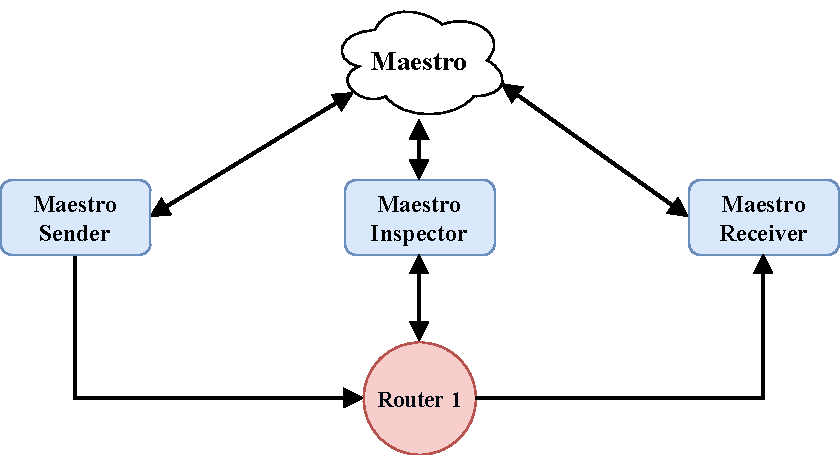
\includegraphics[width=\linewidth]{obrazky-figures/basic_topology_router_single.pdf}}
	\end{minipage}
	\begin{minipage}{0.45\linewidth}
		\subfloat[Topology with a single Broker node.\label{fig:basic_topology_broker}]{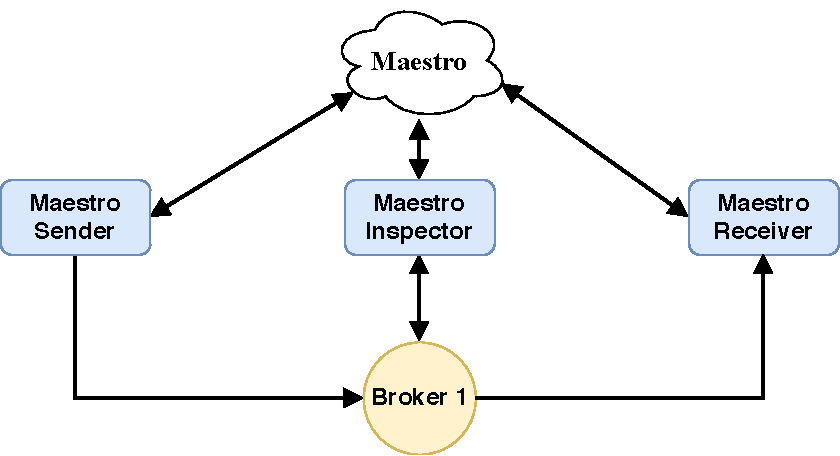
\includegraphics[width=\linewidth]{obrazky-figures/basic_topology_broker_single.pdf}}
	\end{minipage}
	\begin{minipage}{0.45\linewidth}
		\subfloat[Topology consisting of routers nodes only.\label{fig:basic_topology_router_line}]{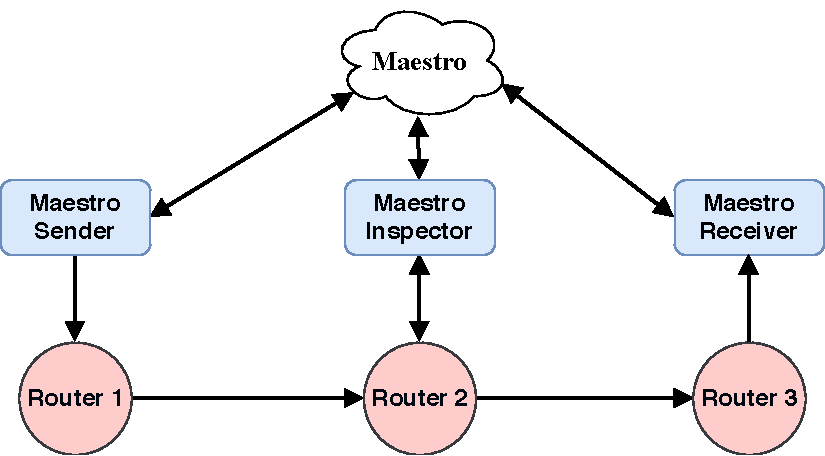
\includegraphics[width=\linewidth]{obrazky-figures/basic_topology_router.pdf}}
	\end{minipage}
	\begin{minipage}{0.45\linewidth}
		\subfloat[Topology with Broker in the middle.\label{fig:basic_topology_broker_line}]{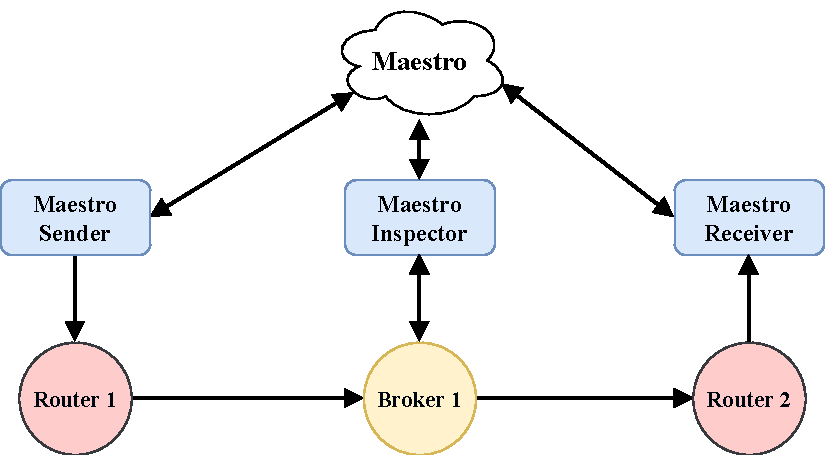
\includegraphics[width=\linewidth]{obrazky-figures/basic_topology_broker.pdf}}
	\end{minipage}
	\caption[Examples of experimental topologies created for basic performance testing and experiments with Maestro.]{Examples of experimental topologies created for basic performance testing and experiments with Maestro. The arrows indicates the communication path between the topology components.}\label{fig:basic_topologies}
\end{figure}

\subsection{Throughput}
\label{Throughput}
We measured throughput only by a load generators\,---\,\emph{Maes\-tro Sender} and \emph{Maestro Receiver}. Load generation depends on the test properties. One can see the test properties for each test case in the Table \ref{tab:test_case_throughput}. Maestro is able to create an unbounded rate test, during which it generates as much load as it can. This type of test was used to reach the maximum handled rate of Qpid-dispatch and Message Broker. The unbound rate during the test is achieved by set environment variable \emph{RATE} to value 0. The throughput test cases are focused on maximum throughput of simple or complex topology.

% Please add the following required packages to your document preamble:
% \usepackage{multirow}
% \usepackage[table,xcdraw]{xcolor}
% If you use beamer only pass "xcolor=table" option, i.e. \documentclass[xcolor=table]{beamer}
\begingroup
\setlength{\tabcolsep}{10pt} % Default value: 6pt
\renewcommand{\arraystretch}{1.35} % Default value: 1
	\begin{table}[H]
	\centering
	\caption{Test case settings for throughput measurements}
	\label{tab:test_case_throughput}
	\begin{tabular}{|l|r|r|r|r|}
	\hline
	\rowcolor[HTML]{C5E3DF}
	\cellcolor[HTML]{C5E3DF}                                         & \multicolumn{4}{c|}{\cellcolor[HTML]{C5E3DF}\textbf{Value}}                                                                          \\ \cline{2-5}
	\rowcolor[HTML]{C5E3DF}
	\cellcolor[HTML]{C5E3DF}                                         & \multicolumn{2}{c|}{\cellcolor[HTML]{C5E3DF}\textbf{Singlepoint}} & \multicolumn{2}{c|}{\cellcolor[HTML]{C5E3DF}\textbf{Multipoint}} \\ \cline{2-5}
	\rowcolor[HTML]{C5E3DF}
	\multirow{-3}{*}{\cellcolor[HTML]{C5E3DF}\textbf{Test Property}} & \textbf{Router}                 & \textbf{Broker}                 & \textbf{Full Router}            & \textbf{With Broker}           \\ \hline
	\textbf{MESSAGE\_SIZE}                                           & \multicolumn{4}{c|}{256}                                                                                                             \\ \hline
	\textbf{PARALLEL\_COUNT}                                         & \multicolumn{4}{c|}{5}                                                                                                               \\ \hline
	\textbf{TEST\_DURATION}                                          & \multicolumn{4}{c|}{15m}                                                                                                             \\ \hline
	\textbf{RATE}                                                    & \multicolumn{4}{c|}{\cellcolor[HTML]{FFFFFF}0}                                                                                       \\ \hline
	\end{tabular}
	\end{table}
\endgroup

\subsubsection*{Single Node}
The first of tests were ran against the single node topologies, which are depicted in the Figures \ref{fig:basic_topology_router} and \ref{fig:basic_topology_broker}. These topologies contains only one SUT node, which are forwarding messages from sender to receiver. During the test is the SUT node inspected by the proper Maestro Inspector.

The measured throughput is depicted in the Figure \ref{fig:rate-single} where one can see the comparison of tests with 15\,minutes duration, which is oriented to achieve highest possible throughput. The one can see that maximum throughput of Qpid-Dispatch as an standalone network component can reach around 90\,0000 messages per second. On the other hand, the lone Messaging Broker reaches only about 30\,000 messages per second. This throughput difference is caused by the fact, that Broker stores all of the messages in the memory till the clients want them. This is main feature of the broker, cause it operates as an message distributor in the network. The router only routes the messages to the destination which does not need to store message in the memory.

\begin{figure}[H]
	\centering
	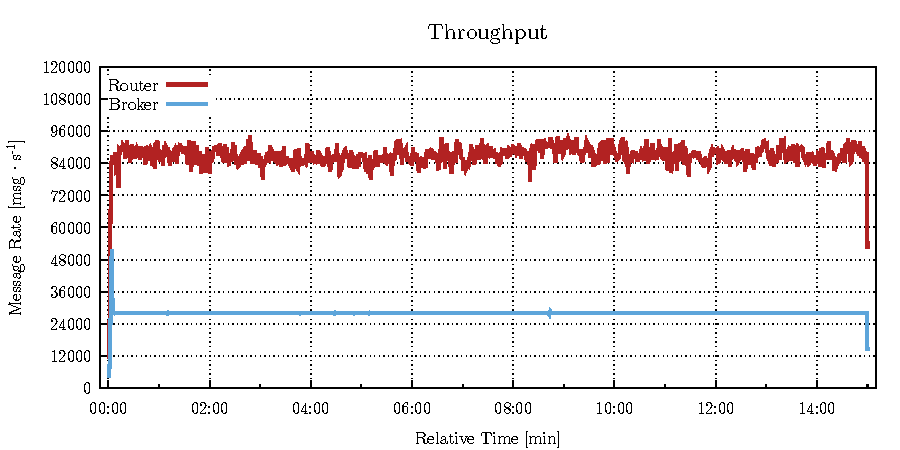
\includegraphics[width=1\linewidth]{obrazky-figures/charts/singlepoint-throughput.pdf}
	\caption{Chart of the maximum throughput of router and broker during the singlepoint test case. One can see here the difference between those two components.}
	\label{fig:rate-single}
\end{figure}

In the Figure \ref{fig:router-single-memory} we can see the memory usage of Qpid-dispatch during the test. We can see here, that totally allocated is around 45\,KB from which is used around 13\,---\,28\,KB. If we compare this with the memory allocation for the Broker, we can see the huge difference between these values. The memory allocated for the Broker is depicted in the Figure \ref{fig:broker-single-memory}. Here we can see that allocated is around 2\,GB of memory and used is around 300\,---\,900\,MB. This is caused by the store message in the memory.

\begin{figure}[H]
	\centering
	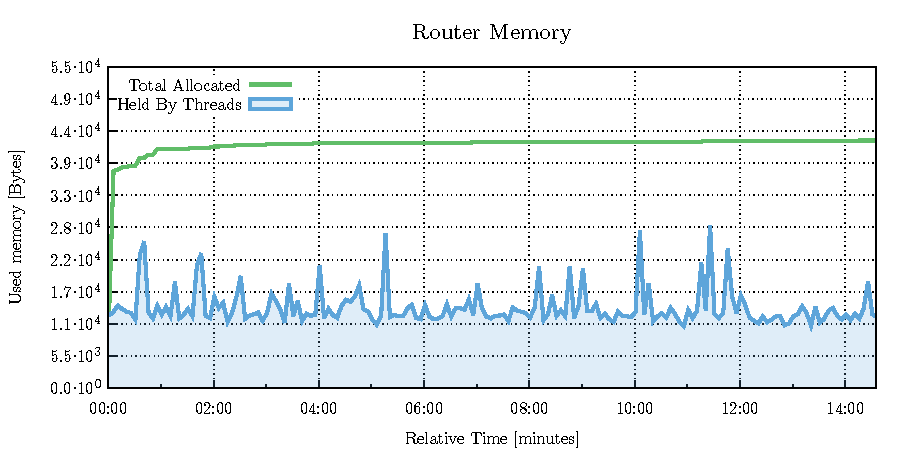
\includegraphics[width=1\linewidth]{obrazky-figures/charts/singlepoint-router-throughput-memory.pdf}
	\caption{The allocated memory and memory in use by Qpid-Dispatch during the test. The data was collected by the inspector every 5\,seconds.}
	\label{fig:router-single-memory}
\end{figure}

\begin{figure}[H]
	\centering
	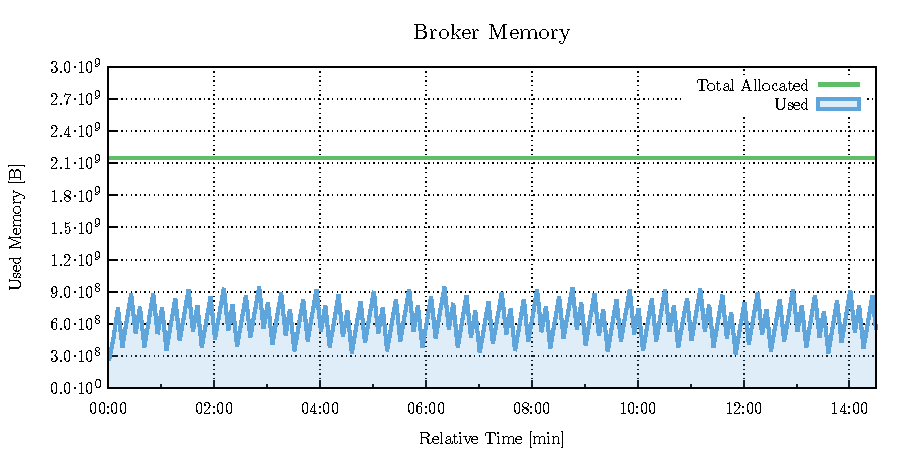
\includegraphics[width=1\linewidth]{obrazky-figures/charts/singlepoint-broker-throughput-memory.pdf}
	\caption{The memory allocation for the Broker service. One can see that the broker allocates more memory than Qpid-Dispatch.}
	\label{fig:broker-single-memory}
\end{figure}


\subsubsection*{Multipoint Topology}
For the multipoint experiments were used topologies depicted in the Figures \ref{fig:basic_topology_router_line} and \ref{fig:basic_topology_broker_line}. The network throughput can be influenced by another devices connected to the topology. The singlepoint topology was extended by another components by add two other routers around the original SUT. The versions of the new added SUTs are the same as the original ones.

\begin{figure}[H]
	\centering
	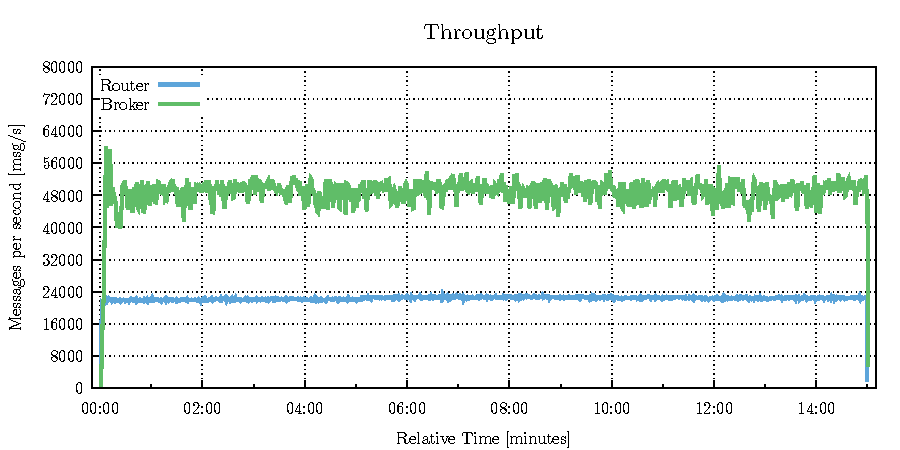
\includegraphics[width=1\linewidth]{obrazky-figures/charts/multipoint-throughput.pdf}
	\caption{Measured throughput of Qpid-Dispatch and Message Broker during the multipoint case study. One can see the performance degradation of Qpid-Dispatch and improvements of Message Broker on that Figure.}
	\label{fig:rate-multipoint-router}
\end{figure}

In the Figure \ref{fig:rate-multipoint-router} one can see, that the adding the routers to the broker node raises achievable throughput to the 48\,000 messages per second. However, the topology consists only of the routers has significant performance degradation. The throughput falls from the 90\,000 messages per second to the approximately 23\,000 messages per second. This degradation is caused by the interior flow-control mechanism, which should prevent the overload of the network. However, in this case study we can see that the performance degradation is too high and the mechanism used in the Qpid-Dispatch should be re-implemented.


\begin{figure}[H]
	\centering
	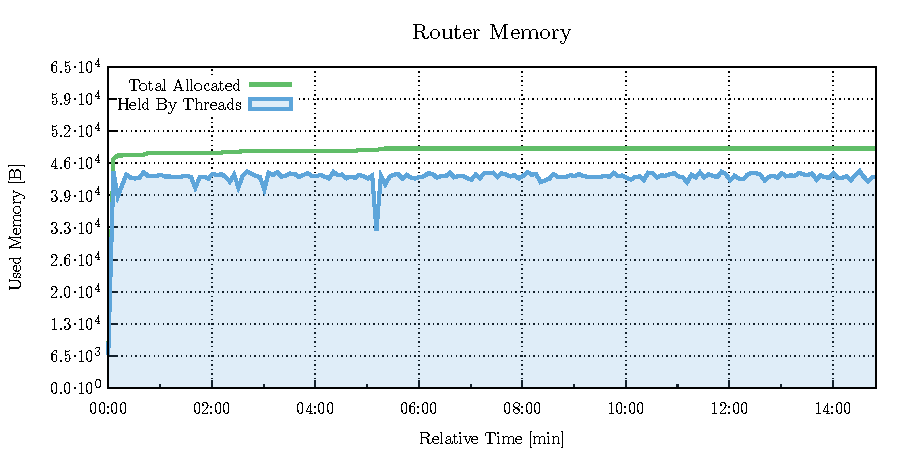
\includegraphics[width=1\linewidth]{obrazky-figures/charts/multipoint-router-only-throughput-memory.pdf}
	\caption{Qpid-Dispatch's memory usage during the multipoint case study. Used memory is higher than in previous case.}
	\label{fig:router-multipoint-memory}
\end{figure}

Based on that mechanism, the memory usage of the middle router depicted in the Figure \ref{fig:router-multipoint-memory} is higher than during the previous case study. Memory used by all threads is there sometimes two times higher and the mean value is around 43\,KB. On the other the, memory allocated for the broker component remains the same as in the previous case study. The memory monitoring for this case study is depicted in the Figure \ref{fig:broker-multipoint-memory}.

\begin{figure}[H]
	\centering
	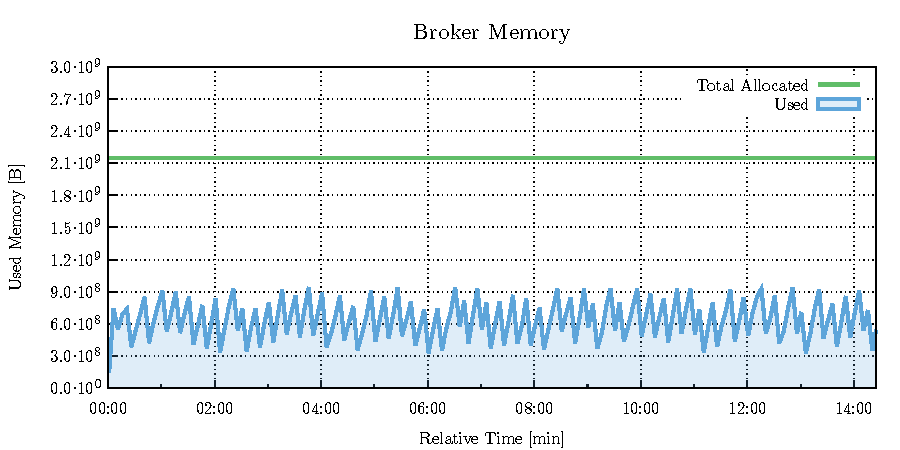
\includegraphics[width=1\linewidth]{obrazky-figures/charts/multipoint-router-broker-throughput-memory.pdf}
	\caption{Memory usage for Broker remains almost the same like in the previous case with less spikes.}
	\label{fig:broker-multipoint-memory}
\end{figure}


\subsubsection*{Conclusion}
The collected data during the throughput measurements reveals unexpected and considerable performance degradation in the serial connection of the Qpid-Dispatch. For comparison between the single and multipoint case study here is the Figure \ref{fig:basic-throughput-comparison}, which puts together all throughput measurements data into one chart. Here one can see the performance improvement between single instance Broker test and the test of topology with the broker (yellow and green color), and performance degradation between router topologies (red and blue color). The results are also available in the Table \ref{tab:throughput-summary}.

% Please add the following required packages to your document preamble:
% \usepackage{multirow}
% \usepackage[table,xcdraw]{xcolor}
% If you use beamer only pass "xcolor=table" option, i.e. \documentclass[xcolor=table]{beamer}
\begingroup
\setlength{\tabcolsep}{10pt} % Default value: 6pt
\renewcommand{\arraystretch}{1.35} % Default value: 1
	\begin{table}[h]
	\centering
	\caption{Table with collected data with highlighted performance improvements and degradations.}
	\label{tab:throughput-summary}
	\begin{tabular}{|l|r|r|r|r|}
	\hline
	\rowcolor[HTML]{C5E3DF}
	\cellcolor[HTML]{C5E3DF}                                         & \multicolumn{2}{c|}{\cellcolor[HTML]{C5E3DF}\textbf{Throughput (Msg/s)}}             & \multicolumn{2}{c|}{\cellcolor[HTML]{C5E3DF}\textbf{Memory}} \\ \cline{2-5}
	\rowcolor[HTML]{C5E3DF}
	\multirow{-2}{*}{\cellcolor[HTML]{C5E3DF}\textbf{Test Type}} & \textbf{Expected}             & \textbf{Measured}                                    & \textbf{Total}              & \textbf{Used max}              \\ \hline
	\textbf{Single Router}                                           & -                             & 90\,000                                                & 45\,MB                       & 28\,MB                          \\ \hline
	\textbf{Single Broker}                                           & -                             & 30\,000                                                & 2\,GB                        & 0.9\,GB                         \\ \hline
	\textbf{Line of Routers}                                         & 90\,000                         & \cellcolor[HTML]{FFCCC9}23\,000                        & 49\,MB                       & 43\,MB                          \\ \hline
	\textbf{Line with Broker}                                        & 30\,000 & \cellcolor[HTML]{9AFF99}48\,000 & 2\,GB                        & 0.9\,GB                         \\ \hline
	\end{tabular}
	\end{table}
\endgroup

\begin{figure}[H]
	\centering
	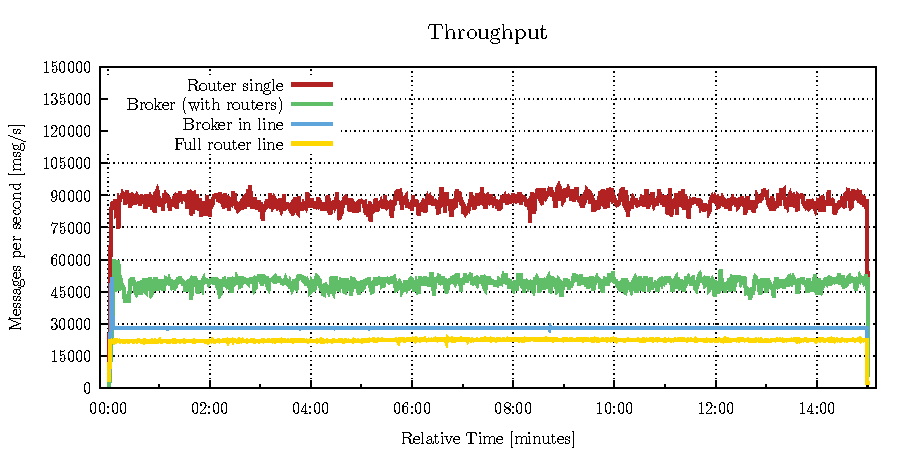
\includegraphics[width=1\linewidth]{obrazky-figures/charts/basic-throughput.pdf}
	\caption{Comparison of all measured throughputs for different components and topologies.}
	\label{fig:basic-throughput-comparison}
\end{figure}


\subsection{Latency}
\label{Latency}
Latency is measured only by Maestro Receiver from certain load samples. Since the Broker is a distribution service, which needs to store messages for some time, or create and keep queues for clients, it has higher requirements for system resources. On the other hand Qpid-dispatch has only one purpose\,---\,to route the messages. This makes it more faster than the Broker. So high load can be unprofitable if one wants better latency during the communication, especially in the case of topology with the broker. The broker can handle less messages than router, but using router can raise broker's throughput since it can control the load. Thus it gives more time to broker to process messages even with higher load. The test cases for latency measurements has slightly different settings than throughput measurement. The settings for this measurements are shown in the Table \ref{tab:test_case_latency}. Note, that \emph{RATE} and \emph{TEST\_DURATION} are sets for each of five connected clients, which means that test is finished after send 10\,000\,000 messages.

% Please add the following required packages to your document preamble:
% \usepackage{multirow}
% \usepackage[table,xcdraw]{xcolor}
% If you use beamer only pass "xcolor=table" option, i.e. \documentclass[xcolor=table]{beamer}
\begingroup
\setlength{\tabcolsep}{10pt} % Default value: 6pt
\renewcommand{\arraystretch}{1.35} % Default value: 1
	\begin{table}[H]
	\centering
	\caption{Test case settings for latency measurements.}
	\label{tab:test_case_latency}
	\begin{tabular}{|l|r|r|r|r|}
	\hline
	\rowcolor[HTML]{C5E3DF}
	\cellcolor[HTML]{C5E3DF}                                         & \multicolumn{4}{c|}{\cellcolor[HTML]{C5E3DF}\textbf{Value}}                                                                          \\ \cline{2-5}
	\rowcolor[HTML]{C5E3DF}
	\cellcolor[HTML]{C5E3DF}                                         & \multicolumn{2}{c|}{\cellcolor[HTML]{C5E3DF}\textbf{Singlepoint}} & \multicolumn{2}{c|}{\cellcolor[HTML]{C5E3DF}\textbf{Multipoint}} \\ \cline{2-5}
	\rowcolor[HTML]{C5E3DF}
	\multirow{-3}{*}{\cellcolor[HTML]{C5E3DF}\textbf{Test Property}} & \textbf{Router}                            & \textbf{Broker}      & \textbf{Full Router}            & \textbf{With Broker}           \\ \hline
	\textbf{MESSAGE\_SIZE}                                           & \multicolumn{4}{c|}{256}                                                                                                             \\ \hline
	\textbf{PARALLEL\_COUNT}                                         & \multicolumn{4}{c|}{5}                                                                                                               \\ \hline
	\textbf{TEST\_DURATION}                                          & \multicolumn{4}{c|}{2\,000\,000}                                                                                                         \\ \hline
	\textbf{RATE}                                                    & \cellcolor[HTML]{FFFFFF}15\,000      & 4\,600                    & 3\,600                    & 7\,600                   \\ \hline
	\end{tabular}
	\end{table}
\endgroup

\subsubsection*{Single Node}
The latency measurements are done with 80\% of maximum rate measurements, which were discussed in the Subsection \ref{Throughput}. In the Figure \ref{fig:latency-single-router} you can see the latency difference that we measured between Qpid-Dispatch and Message Broker. In single node measurements, the router's latency is slightly higher in the most of the cases. This is caused by the Maestro Sender and Receiver technology, because they are implemented in Java and Maestro Sender and Receiver using JMS for send an receive message, which is same approach as the Broker uses. For better latency comparison is necessary to measure Broker's latency with current implementations and Qpid-Dispatch's latency with Python clients. However, current version of Maestro offers only the JMS clients.

\begin{figure}[H]
	\centering
	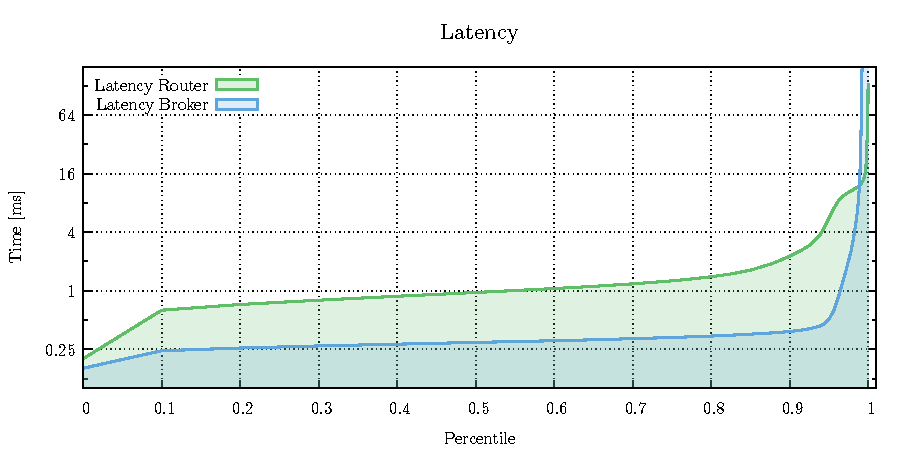
\includegraphics[width=1\linewidth]{obrazky-figures/charts/singlepoint-latency.pdf}
	\caption{Latency chart showing the difference between the router and the broker latency at 80\,\% of maximum rate. One can see that router is slower, but this is caused by the technology used in the Maestro Clients which is same as in the Broker..}
	\label{fig:latency-single-router}
\end{figure}

The memory used by Qpid-dispatch is slightly lower and much stable than in the case of maximum throughput as one can see in the Figure \ref{fig:latency-single-router-memory}. This proves, that used memory is mild to the  load. If the load on the router is higher than it needs more memory for proper routing. In the Figure \ref{fig:latency-single-broker-memory} one can see the Inspector output for Broker's used memory. The used memory is here much stable then in the previous cases, which is caused, as in the router case, by lower load on the Broker. Maximum used memory is same as in the previous cases.

\begin{figure}[H]
	\centering
	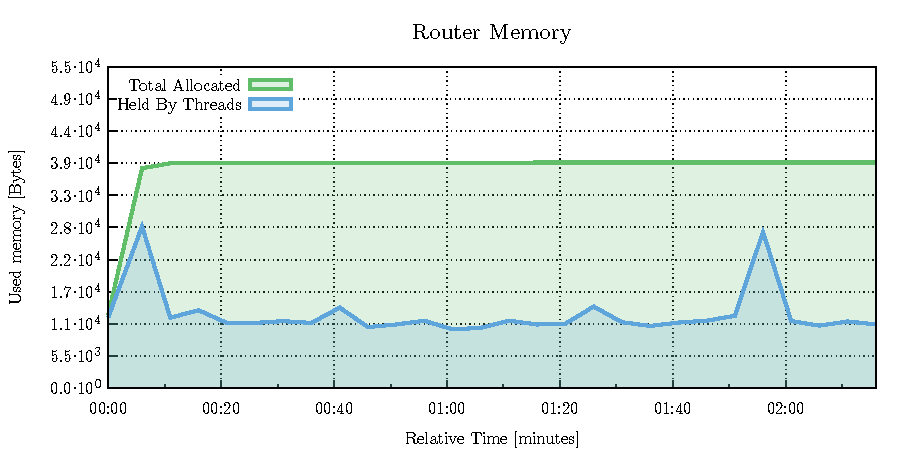
\includegraphics[width=1\linewidth]{obrazky-figures/charts/singlepoint-router-latency-memory.pdf}
	\caption{Memory usage of Qpid-Dispatch is much stable when the router is not under the maximum load. The spikes are caused by some unexpected events in the topology.}
	\label{fig:latency-single-router-memory}
\end{figure}

\begin{figure}[H]
	\centering
	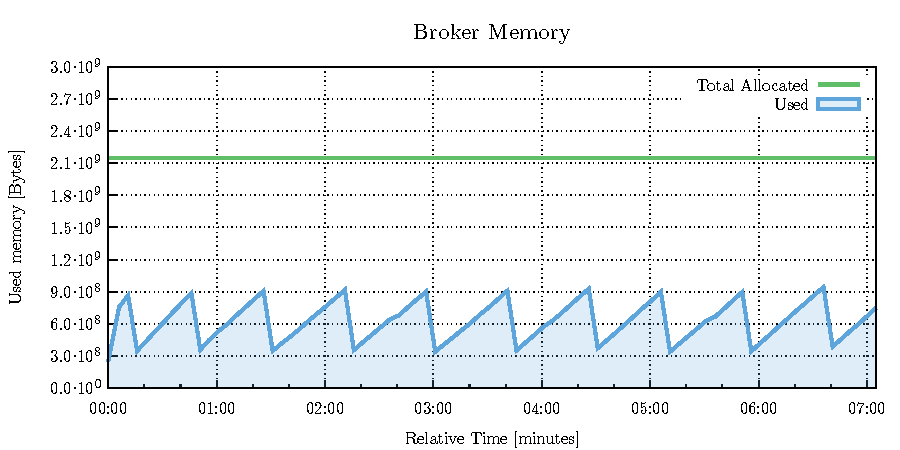
\includegraphics[width=1\linewidth]{obrazky-figures/charts/singlepoint-broker-latency-memory.pdf}
	\caption{The Broker's memory usage has lesser spike when the load is only about of 80\,\% of maximum.}
	\label{fig:latency-single-broker-memory}
\end{figure}

\subsubsection*{Multipoint Topology}
One can see the measured latency on multinode topology of three routers, and two routers with middle-broker in the Figure \ref{fig:latency-multipoint-router}. The latency curve proves, that routers are able to deliver messages into its destination faster than topology with the Broker, because the Broker needs to store them in the memory. The latency of the topology with broker reaches around 16\,$\mu$s in 90\,\% of samples; on the other hand, topology consisting of routers has significantly better latency that is around 1\,$\mu$s in 90\,\% of samples. The conclusion is that the collected data proves the router should be much faster than the broker during the certain circumstances..

\begin{figure}[H]
	\centering
	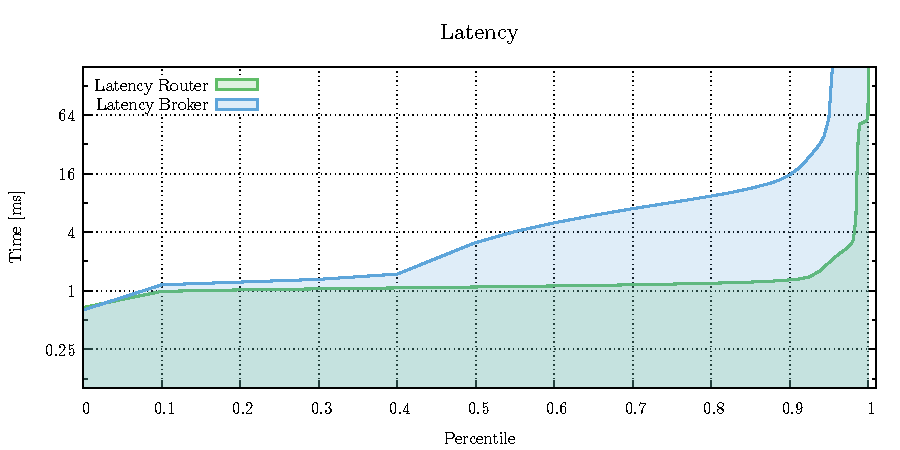
\includegraphics[width=1\linewidth]{obrazky-figures/charts/multipoint-latency.pdf}
	\caption{Latency comparison between topologies with only routers and with the middle-broker. The router network is here significantly faster.}
	\label{fig:latency-multipoint-router}
\end{figure}

\begin{figure}[H]
	\centering
	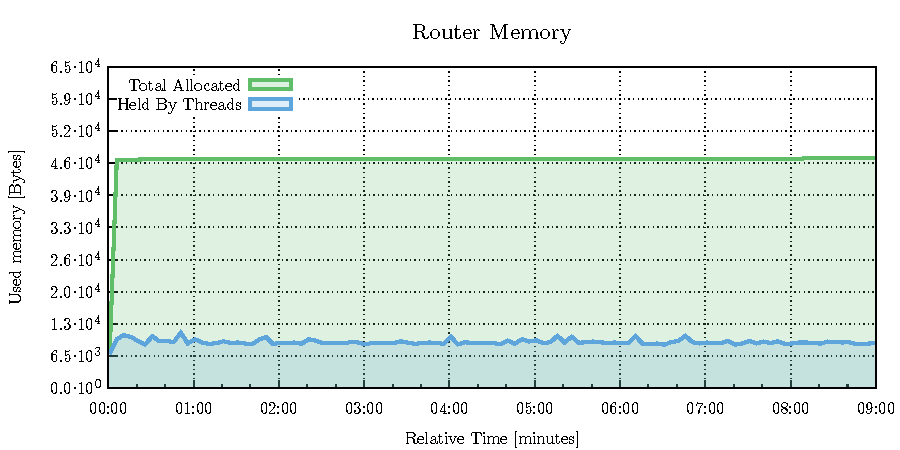
\includegraphics[width=1\linewidth]{obrazky-figures/charts/multipoint-router-only-latency-memory.pdf}
	\caption{Memory usage shows, that memory usage of the router is affected by the throughput.}
	\label{fig:latency-multiple-router-memory}
\end{figure}

Collected data about the memory usage proves the previous statements. In the Figure \ref{fig:latency-multiple-router-memory} is shown used memory by Qpid-Dispatch. The curve is very stable and the values moves around the 9\,MB of used memory. The used memory by the Broker shown in the Figure \ref{fig:latency-multiple-broker-memory} is very similar as in the previous measurements.

\begin{figure}[H]
	\centering
	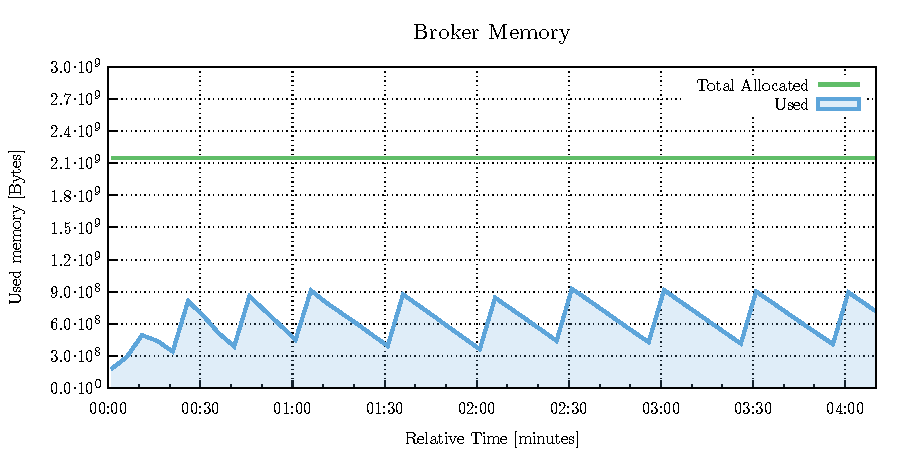
\includegraphics[width=1\linewidth]{obrazky-figures/charts/multipoint-router-broker-latency-memory.pdf}
	\caption{Chart of memory allocation on the Broker node..}
	\label{fig:latency-multiple-broker-memory}
\end{figure}

\subsubsection*{Conclusion}
During the latency measurements we collected and compared data for the Qpid-Dispatch and Message Broker topologies. The summary of latency measurements is available in the Table \ref{tab:latency-summary}. Is it was already mentioned, Qpid-Dispatch is faster in the model environment the Message Broker. How to achieve better comparison of latency measurements is discussed in the Section \ref{Maestro Clients in Python} as a part of possible improvements.

% Please add the following required packages to your document preamble:
% \usepackage{multirow}
% \usepackage[table,xcdraw]{xcolor}
% If you use beamer only pass "xcolor=table" option, i.e. \documentclass[xcolor=table]{beamer}
\begingroup
\setlength{\tabcolsep}{10pt} % Default value: 6pt
\renewcommand{\arraystretch}{1.35} % Default value: 1
	\begin{table}[H]
	\centering
	\caption{Table with collected latency data with highlighted performance improvements and degradations.}
	\label{tab:latency-summary}
	\begin{tabular}{|l|r|r|r|r|r|}
	\hline
	\rowcolor[HTML]{C5E3DF}
	\multicolumn{1}{|c|}{\cellcolor[HTML]{C5E3DF}}                                     & \multicolumn{2}{c|}{\cellcolor[HTML]{C5E3DF}\textbf{Latency (us)}}                                                        & \multicolumn{2}{c|}{\cellcolor[HTML]{C5E3DF}\textbf{Memory}}                                                                 & \multicolumn{1}{c|}{\cellcolor[HTML]{C5E3DF}}                                                                                         \\ \cline{2-5}
	\rowcolor[HTML]{C5E3DF}
	\multicolumn{1}{|c|}{\multirow{-2}{*}{\cellcolor[HTML]{C5E3DF}\textbf{Test Type}}} & \multicolumn{1}{c|}{\cellcolor[HTML]{C5E3DF}\textbf{90 \%}} & \multicolumn{1}{c|}{\cellcolor[HTML]{C5E3DF}\textbf{99 \%}} & \multicolumn{1}{c|}{\cellcolor[HTML]{C5E3DF}\textbf{Total}} & \multicolumn{1}{c|}{\cellcolor[HTML]{C5E3DF}\textbf{Used max}} & \multicolumn{1}{c|}{\multirow{-2}{*}{\cellcolor[HTML]{C5E3DF}\textbf{\begin{tabular}[c]{@{}c@{}}Duration \\ (seconds)\end{tabular}}}} \\ \hline
	\textbf{Single Router}                                                             & 2.263                                                       & 12.495                                                      & 38 KB                                                       & 28 KB                                                          & \cellcolor[HTML]{9AFF99}136                                                                                                           \\ \hline
	\textbf{Single Broker}                                                             & 0.386                                                       & 181.759                                                     & 2 GB                                                        & 0.9 GB                                                         & \cellcolor[HTML]{FFCCC9}425                                                                                                           \\ \hline
	\textbf{Line of Routers}                                                           & \cellcolor[HTML]{9AFF99}1.292                               & 50.815                                                      & 46 KB                                                       & 8 KB                                                           & \cellcolor[HTML]{FFCCC9}540                                                                                                           \\ \hline
	\textbf{Line with Broker}                                                          & \cellcolor[HTML]{FFCCC9}15.487                              & 1031.167                                                    & 2 GB                                                        & 0.9 GB                                                         & \cellcolor[HTML]{9AFF99}250                                                                                                           \\ \hline
	\end{tabular}
	\end{table}
\endgroup

\newpage
\section{Behavior Measurements}
\label{Behavior Measurements}

\todo{Tohle popsat az s~nejakym dalsim merenim, zatim asi netreba kontrlovat, pouze prevzato z~Excelu}

\subsection{Agent Evaluation}
Moreover, we present some preliminary results with using the agent extension and changing the behavior of topology depicted in the Figure \ref{fig:basic_topologies}. In the Figure \ref{fig:agent_throughput} you can see throughput of few simple tests during which middle router is restarted or shut down. The throughput spikes are caused by these events. Since router does not have any queues to store messages, the messages are then discarded and lost. However, the sender does not receive acknowledgment of lost messages so it is not router responsibility. In the Table \ref{tab:agent_simple} you can see the duration of each executed operation and rate of lost messages during the operation (with expected amount of messages being 10\,000\,000). For example during the restart, router was completely shutdown for a second during which no messages arrived. However, after the restart there was some time to balance the load to the previous point. This leads to message lost equals to 2 seconds rate.

% Please add the following required packages to your document preamble:
% \usepackage[table,xcdraw]{xcolor}
% If you use beamer only pass "xcolor=table" option, i.e. \documentclass[xcolor=table]{beamer}
\begin{table}[H]
\centering
\caption{Summarization of lost messages during the connection issues.}
\label{my-label}
\begin{tabular}{|c|r|r|}
\hline
\rowcolor[HTML]{C5E3DF}
Operation     & Duration (seconds) & Message Lost \\ \hline
None          & 0        & None         \\ \hline
Restart       & 1        & 46437        \\ \hline
Shutdown      & 12       & 280572       \\ \hline
Long Shutdown & 89       & 1304451      \\ \hline
\end{tabular}
\label{tab:agent_simple}
\end{table}

The Figure \ref{fig:agent_throughput} also shows, that test case with long shutdown is longer about 10 seconds that other scenarios and the throughput after the shutdown is quite higher. This means that router high throughput to even the messages lost.

\begin{figure}[H]
	\centering
	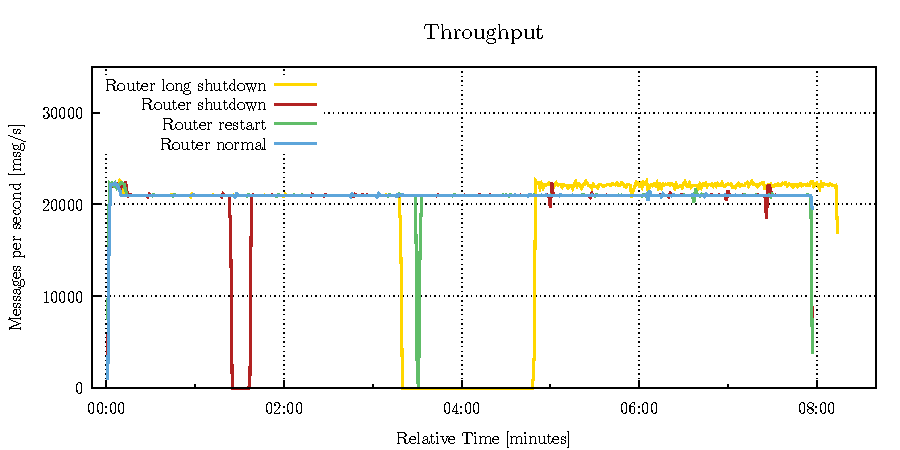
\includegraphics[width=1\linewidth]{obrazky-figures/charts-excel/agent.pdf}
	\caption{Router throughput comparison during the same load after different unexpected events.}
	\label{fig:agent_throughput}
\end{figure}

Latency of test cases cases with the agent function demonstration is depicted in the Figure \ref{fig:agent_latency}. You can see that router is able to even the latency during the restart and short shutdown with test run without any unexpected behavior. On the other hand, long shutdown (red) gets worse latency almost for 50 percentile of messages.

\begin{figure}[H]
	\centering
	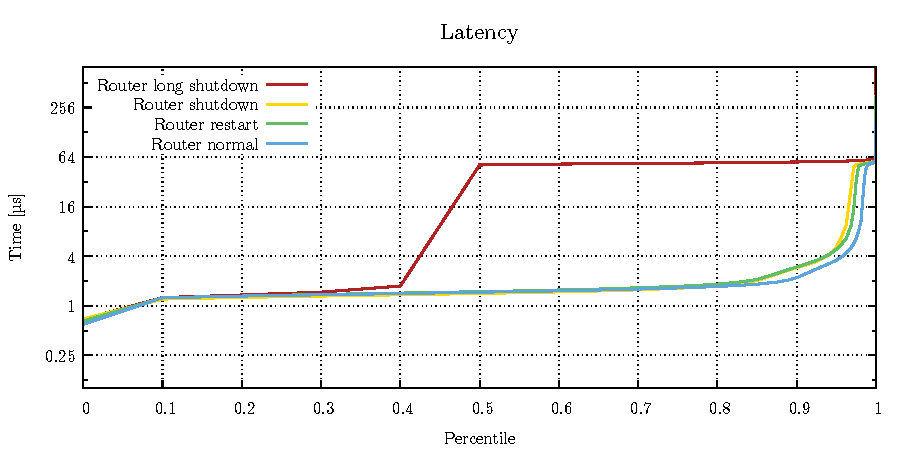
\includegraphics[width=1\linewidth]{obrazky-figures/charts-excel/agent_latency.pdf}
	\caption{Router and broker latency comparison during the same load.}
	\label{fig:agent_latency}
\end{figure}


\section{Problems}

All measurements were orchestrated by an automation server called Jenkins\footnote{Jenkins\,---\,\url{https://jenkins.io/}}.

  % (c) Jakub Stejskal
% Master Thesis
% Performance Testing and Analysis of Qpid-Dispatch Router
% Chapter 7

\chapter{Future works and ideas}
\label{Future works and ideas}
The Maestro is currently used for performance testing of Apache ActiveMQ Artemis and Qpid-Dispatch in Red Hat Messaging QE team. This makes the Maestro one of the key utilities for the Messaging and the primary performance tool. But since the Maestro is basically immature system, there is still a lot of places for improvements. We present several ideas in the following. Note, that Maestro-Agent and AMQP Inspector are new Maestro modules, which makes performance testing of Qpid-Dispatch with collecting interior data about SUT itself available. These extensions were already merged in the upstream and are available since Maestro stable version 1.3.0.

\section{Regression Testing}
Since both message broker and message router have new builds every few weeks, there can occur a performance degradation. This issue can be caused by just one simple commit, which can fix some issues but break performance. However, Maestro can catch such performance degradation early in the process, if there is already previously measured data with specific informations (so called baselines). Maestro can then re-run the same test with new version of SUT and compare the collected results with previous the data set.

This mechanism is simple to achieve. The first step is to configure the pipeline job on the orchestration and integration system such as Jenkins or Travis CI. This job has to have access to SUT repository and baseline data tagged as a performance standard for the SUT. The trigger of this pipeline can be every push or every commit with specific tag. The other step is the extension of the Maestro-Reporter, where it can compare older data with newly collected ones and report, how much they differ and where. This pipeline job then can alert engineers, that some specific commit caused performance degradation and also show the difference between actual collected data and estimate collected data.

This type of testing can also be applicable to all test cases with different SUT configuration. The Maestro would be able to compare expected data with collected data and tell us that this specific configuration has a performance degradation.

\section{Data Reporting}
The current reports, created by Maestro itself, contain charts, in the \emph{png} format generated by the Java library for creating bitmap figures. This makes them less informative that they could be with better data visualization. Since Inspectors collect additional data about SUT, e.g. memory usage, it will be helpful for engineers of SUT to see interactive charts with collected data. With this options, engineers can better analyze what is going on with SUT during the test scenario.

A~good example of interactive and vector charts library is \emph{Grafana}\footnote{Grafana\,---\,open source software for time series analytics \url{https://grafana.com/}}. Grafana can produce awesome outputs from collected data e.g. from the database. Another example is \emph{Project Jupyter}\footnote{Jupyter\,---\,\url{http://jupyter.org/}}, which can plot interactive charts from database source data on the fly. One only needs installed Python on the node. Jupyter starts a Python server on the node and makes plotted data available via the HTTP browser. Maestro can implement such strategy, as a new peer similar to the data server code, which is running on all Maestro peer nodes. The difference is, that this report server will be started by Maestro-Reporter on the execution node.

\section{Collected Data Compression}
Each Maestro peer collects different data during the test. Size of these data is based on peer type, collected data format and test duration. For example the Maestro-Receiver collects huge amount of time for throughput and latency chart. These data are represented as a double-column csv file with columns \emph{eta}(estimated time of arrival) and \emph{ata}(actual time of arrival). Each csv file looks like the following:

\begin{verbatim}
  eta;ata
  "2017-10-19 13:19:32.661300","2017-10-19 13:19:32.706649"
  "2017-10-19 13:19:32.661500","2017-10-19 13:19:32.706823"
\end{verbatim}

Imagine, that this record is written for each send/received message on sender or receiver. For example we can have 50,000 records with prefix \texttt{"2017-10-19 13:19:32"} which represents a huge redundancy. The idea of compression is to save only first timestamp and then compute difference between saved timestamp and current timestamp and write this difference into csv file. This way would be able to save at least 15\,B per timestamp, which saves more than one half of current size. The only necessary thing is to write a new timestamp after some time, when difference is too big. The new csv file would then look like the following:

\begin{verbatim}
  eta;ata
  1525285541559,+18787
  +30,+40
  +35,+42
\end{verbatim}

\section{Multi-point Senders and Receiver}
Behavioral testing introduces an idea of multipoint senders and receivers. Lets say, that we want to collect behavioral data about Qpid-Dispatch with two queues, where the first queue accepts messages from two senders and the second queue accepts messages from five senders. This situation better simulates the real network traffic than the current mechanism. To achieve this, the Maestro needs to extend Maestro-Worker with option for multiple endpoint connections dynamically. The current version offers only one specific connection specified by the user.

\section{Maestro-Agent Executor Improvements}
The Maestro-Agent is able to download external git repositories and tries to process them during the test. However, the external code handler is currently designed only for code written in Groovy. This limitation can be easily removed by creating more general executor, which would be able to execute any type of scripts. One idea how to achieve this is to create more complex executor in \emph{Kotlin} languange\footnote{Kotlin\,---\,\url{https://kotlinlang.org/}}. The new executor should be able to run each type of downloaded script and keep the access to the return code and standard output. This extension would remove the limitation to use, which has to specify each external action handler in the Groovy language. Note, that new executor should not affect performance testing during the execution, so the operations should remain atomic.

\section{Multiple Agents and Inspectors}
Version of Maestro 1.3.0 has already integrated Maestro Agent and AMQP Inspector. However, the front-end API does not allows setting for multiple Agents or Inspectors during one test scenario. Hence, only one Agent and one Inspector can be specified by Groovy test script. The solution for this problem must involve dynamic scan of specific environment variables which will contains setting for the Maestro components. The settings can be loaded into the array of Agent/Inspector setting and then can be assigned to a specific component by the node URL.

% \section{Problems}
% \todo{Todo - popsat nebo vypustit?}
% \begin{itemize}
%   \item \textbf{Jenkins}\,---\,the idea was to have jobs in Jenkins\footnote{Jenkins\,---\,\url{https://jenkins.io/}} but Maestro does not like Jenkins without reason, probably some hidden issue
%   \item \textbf{QpidJMS}\,---\,QpidJMS is not able to fill MapMessage body by default only via undocumented feature, the developer consultaiton was needed.
%   \item \textbf{Qpid-Dispatch}\,---\,performance degradation in line topology was discussed with engineers and it was said: "it is ok, it's flow control".
%   \item \textbf{Agent and Inspector on same node}\,---\,this sometimes cause the problem (caused by data server which is binded to node) that test will not be ended properly (try it).
% \end{itemize}

  % (c) Jakub Stejskal
% Master Thesis
% Performance Testing and Analysis of Qpid-Dispatch Router
% Chapter 8

\chapter{Conclusion}
\label{Conclusion}
In this work we described the fundamentals of performance testing, common performance metrics and bugs, and selected related tools. Further, we introduced the architecture and functionality of Messaging Performance Tool (MPT) called Maestro. The main part of this work focused on the proposal and implementation of extensions for Maestro, in particular new components: Maestro Agent and AMQP Inspector. The implementation of these components was necessary to enable proper performance testing of Qpid-Dispatch router. Moreover, we designed and implemented the Topology Generator tool, which is going to be used for semi-automatic topology configuration generation, which will significantly simplify the testing phase.

% The design was changed multiple times during this work according the needs of the performance testing of Qpid-Dispatch but also of Maestro itself. For example the Maestro Agent was initially designed as a component which can control the router, but after some discussions and implementation start we decided to create Maestro Agent as independent code handler on the SUT node. This allows router control, but also control of any other software on the node easily by external Groovy scripts available in any public git repository.
%
% AMQP Inspector was added to the design after the Agent development when we realized that is more efficient to create a new component for router inspection. It is possible to use Maestro Agent and parse the string output of external tool which can inspect the router, but it is not comfortable to send the long output through the Maestro Broker and then parse it. The result was the AMQP Inspector as a new component, which only need path to the router and then is able to collect and parse data about the SUT.

Implemented extensions were experimentally evaluated on series of basic and behavioral test cases. We performed the collection of performance data of several topologies generated by Topology Generator. While we decided to pick small topologies they still can offers interesting results about the performance of Qpid-Dispatch and we compared the results with Message Broker component. The experimental evaluation has shown some interesting data and has discovered several performance degradations.

The code of the work is published as an open-source repository and is available on GitHub. All developed extensions were already merged into the upstream version of Maestro and will be available since the version 1.3.0, which is already used for performance testing of MOM by Red Hat company. The preliminary results of this work were presented and published in the paper for Excel@FIT\footnote{Excel@FIT\,---\,IT conference for students and theirs work \url{http://excel.fit.vutbr.cz/}} conference.

%During term project is collected relative information about performance testing. This information are processed and recorded in this work in the Chaper \ref{Fundamentals of Software Performance Testing}. I~also get introduction into functionality of Messaging Performance Tool which is going to be upgraded and used for performance testing of Qpid-Dispatch. In the Chaper \ref{Analysis and Design} I~summarized design of necessary upgrades for MPT and design of Topology Generator which going to be used for semi-automatic topology configuration generation and together with automatic deployment on testing nodes. Topology is currently implemented, tested and published under version 0.1.10. Current version is able to generate any topology by manner as is described in the Chapter \ref{Analysis and Design}. Link to public source-code is available in \ref{Topology Generator Source Code}.

%Next step of this thesis will lead to implement module for Qpid-Dispatch performance testing, integrated it into MPT and improved Topology Generator.After this, I~will be ready for proper performance testing of Qpid-Dispatch with data analysis.

%=========================================================================


  % Kompilace po částech (viz výše, nutno odkomentovat)
  % Compilation piecewise (see above, it is necessary to uncomment it)
  %\subfile{projekt-01-uvod-introduction}
  % ...
  %\subfile{chapters/projekt-05-conclusion}


  % Pouzita literatura / Bibliography
  % ----------------------------------------------
\ifslovak
  \makeatletter
  \def\@openbib@code{\addcontentsline{toc}{chapter}{Literatúra}}
  \makeatother
  \bibliographystyle{bib-styles/slovakiso}
\else
  \ifczech
    \makeatletter
    \def\@openbib@code{\addcontentsline{toc}{chapter}{Literatura}}
    \makeatother
    \bibliographystyle{bib-styles/czechiso}
  \else
    \makeatletter
    \def\@openbib@code{\addcontentsline{toc}{chapter}{Bibliography}}
    \makeatother
    \bibliographystyle{bib-styles/englishiso}
  %  \bibliographystyle{alpha}
  \fi
\fi
  \begin{flushleft}
  \bibliography{xstejs24-performance-20-literatura-bibliography}
  \end{flushleft}

  % vynechani stranky v oboustrannem rezimu
  % Skip the page in the two-sided mode
  \iftwoside
    \cleardoublepage
  \fi

  % Prilohy / Appendices
  % ---------------------------------------------
  \appendix
\ifczech
  \renewcommand{\appendixpagename}{Přílohy}
  \renewcommand{\appendixtocname}{Přílohy}
  \renewcommand{\appendixname}{Příloha}
\fi
\ifslovak
  \renewcommand{\appendixpagename}{Prílohy}
  \renewcommand{\appendixtocname}{Prílohy}
  \renewcommand{\appendixname}{Príloha}
\fi
%  \appendixpage

% vynechani stranky v oboustrannem rezimu
% Skip the page in the two-sided mode
%\iftwoside
%  \cleardoublepage
%\fi

  \ifODSAZ
    \setlength{\parskip}{0.5\bigskipamount}
  \else
    \setlength{\parskip}{0pt}
  \fi

  % vynechani stranky v oboustrannem rezimu
  \iftwoside
    \cleardoublepage
  \fi

  % Seznam obrazku a tabulek (pokud prace obsahuje velke mnozstvi obrazku, tak se to hodi)
  % List of figures and list of tables (if the thesis contains a lot of pictures, it is good)
  \ifczech
    \renewcommand\listfigurename{Seznam obrázků}
  \fi
  \ifslovak
    \renewcommand\listfigurename{Zoznam obrázkov}
  \fi
  \listoffigures

  \ifczech
    \renewcommand\listtablename{Seznam tabulek}
  \fi
  \ifslovak
    \renewcommand\listtablename{Zoznam tabuliek}
  \fi
  \listoftables

  \ifODSAZ
    \setlength{\parskip}{0.5\bigskipamount}
  \else
    \setlength{\parskip}{0pt}
  \fi

  % Tento soubor nahraďte vlastním souborem s přílohami (nadpisy níže jsou pouze pro příklad)
% This file should be replaced with your file with an appendices (headings below are examples only)

% Umístění obsahu paměťového média do příloh je vhodné konzultovat s vedoucím
% Placing of table of contents of the memory media here should be consulted with a supervisor
%\chapter{Obsah přiloženého paměťového média}

\chapter*{List of Shortcuts}
\begingroup
\setlength{\tabcolsep}{10pt} % Default value: 6pt
\renewcommand{\arraystretch}{1.5} % Default value: 1
  \begin{tabular}{rl}
    \textbf{MPT} & Messaging Performance Tool \\
    \textbf{KPI} & Key Performance Indicators \\
    \textbf{CPU} & Central processing unit \\
    \textbf{SUT} & System Under Test \\
    \textbf{AMQP} & Advanced Message Queuing Protocol \\
    \textbf{MOM} & Message-oriented middleware \\
    \textbf{STOMP} & Streaming Text Oriented Messaging Protocol \\
    \textbf{OpenWire} & Cross language wire protocol \\
    \textbf{REST} & Representational State Transfer \\
    \textbf{JVM} & Java Virtual Machine \\
    \textbf{JMX} & Java Management Extensions \\
    \textbf{SASL} & Simple Authentication and Security Layer \\
    \textbf{SSL/TLS} & Secure Sockets Layer/Transport Layer Security \\
    \textbf{MQTT} & Message Queuing Telemetry Transport \\
    \textbf{ISO/OSI} & Open Systems Interconnection model \\
    \textbf{OSPF} & Open Shortest Path First \\
    \textbf{IS-IS} & Intermediate System to Intermediate System \\
    \textbf{IP} & Internet Protocol \\
    \textbf{RTT} & Round Trip Time \\
    \textbf{CSV} & Comma-separated Values \\
    \textbf{PNG} & Portable Network Graphics \\
  \end{tabular}
\endgroup

  \newpage

  \ifslovak
  %  \section*{Zoznam príloh}
  %  \addcontentsline{toc}{section}{Zoznam príloh}
  \else
    \ifczech
     \section*{Seznam příloh}
     \addcontentsline{toc}{section}{Seznam příloh}
    \else
     \section*{List of Appendices}
     \addcontentsline{toc}{section}{List of Appendices}
    \fi
  \fi
    \startcontents[chapters]
    \setlength{\parskip}{0pt}
    % seznam příloh / list of appendices
    \printcontents[chapters]{l}{0}{\setcounter{tocdepth}{2}}

  % Přílohy / Appendices
  % Tento soubor nahraďte vlastním souborem s přílohami (nadpisy níže jsou pouze pro příklad)
% This file should be replaced with your file with an appendices (headings below are examples only)

% Umístění obsahu paměťového média do příloh je vhodné konzultovat s vedoucím
% Placing of table of contents of the memory media here should be consulted with a supervisor
%\chapter{Obsah přiloženého paměťového média}

%\chapter{Manuál}
\chapter{The Maestro Protocol}

\section{The Maestro Commands}
\label{AP:commands}
\todo{\url{https://github.com/orpiske/msg-perf-tool/tree/master/doc/maestro/protocol}}

\chapter{Topology Generator} % Configuration file

\section{Inventory}
\label{AP:Inventory}
An example of Inventory file for Topology Generator and Ansible deployment scripts.

\begin{verbatim}
[clients]
sender ansible_host=10.0.0.1					
receiver ansible_host=10.0.0.2

[routers]
router1 ansible_host=10.0.0.3
router2 ansible_host=10.0.0.4

[brokers]
broker1 ansible_host=10.0.0.5

[nodes:children]
brokers
clients
routers
\end{verbatim}

\section{Graph Metadata}
\label{AP:Graph Metadata}
Example of graph metadata file for Topology Generator. Generator will generate graph with 2 routers and 3 brokers where routers are connected together and each broker is connected to one router.

\begin{verbatim}
---
directed: false
graph: {}
nodes:
- type: router						%node type
  id: router1						%node name
- type: router
  id: router2
- type: broker
  id: broker1
- type: broker
  id: broker2
links:
- source: router2					%source node for link
  target: router1					%target node for link
- source: router2
  target: broker2
- source: router1
  target: broker1
multigraph: false
\end{verbatim}

\section{Topology Generator Output}
\label{AP:Topology Generator Output}
Example of Topology Generator output in YAML format. This output is for two directly connected routers.

\begin{verbatim}
---
confs:
- machine: router1
  router:
  - id: router1
    mode: standalone
  listener:
  - host: 0.0.0.0
    role: inter-router
    port: 6000
  - host: 0.0.0.0
    authenticatePeer: 'no'
    role: normal
    port: 5000
    saslMechanisms: ANONYMOUS
  connector:
  - host: router2
    role: inter-router
    port: 6001
  address:
  - prefix: closest
    distribution: closest
  - prefix: multicast
    distribution: multicast
  - prefix: unicast
    distribution: closest
- machine: router2
  router:
  - id: router2
    mode: standalone
  listener:
  - host: 0.0.0.0
    role: inter-router
    port: 6001
  - host: 0.0.0.0
    authenticatePeer: 'no'
    role: normal
    port: 5001
    saslMechanisms: ANONYMOUS
  connector:
  - host: router1
    role: inter-router
    port: 6000
  address:
  - prefix: closest
    distribution: closest
  - prefix: multicast
    distribution: multicast
  - prefix: unicast
    distribution: closest

\end{verbatim}

\section{Qpid-Dispatch Configuration File Template}
\label{AP:Qpid-Dispatch Configuration File Template}
Template for configuration files for current version of Qpid-Dispatch is available at \url{https://github.com/rh-messaging-qe/ansible-qpid-dispatch/blob/master/test/files/templates/qdrouterd-roland.conf.j2}.

\section{Topology Generator Source Code}
\label{AP:Topology Generator Source Code}
Complete source code of Topology Generator is available at \url{https://github.com/rh-messaging-qe/iqa-topology-generator}.

%\chapter{RelaxNG Schéma konfiguračního souboru} % Scheme of RelaxNG configuration file

%\chapter{Plakát} % poster


  % Kompilace po částech (viz výše, nutno odkomentovat)
  % Compilation piecewise (see above, it is necessary to uncomment it)
  %\subfile{projekt-30-prilohy-appendices}

\end{document}
